% =====================================================================
%  MSDM 5053 -- Group Project Report
%  Topic: Time-Series Analysis of Four Hong Kong Stocks (2011-2024)
%  Compile: pdflatex -shell-escape report.tex  (run twice for refs)
%
%  Asset paths assume this file lives in   d:/Downroads/project5053/report/
%  and figures/tables come from           ../output/<ticker>/...
% =====================================================================
\documentclass[11pt,a4paper]{article}

% ---------- packages ----------
\usepackage[T1]{fontenc}
\usepackage[utf8]{inputenc}
\usepackage[margin=1in]{geometry}
\usepackage{graphicx}
\usepackage{booktabs}
\usepackage{amsmath, amssymb}
\usepackage{caption}
\usepackage{subcaption}
\usepackage{float}
\usepackage{csvsimple}        % \csvautotabular for CSV -> LaTeX table
\usepackage{listings}         % code listings in appendix
\usepackage{xcolor}
\usepackage{hyperref}
\usepackage{underscore}    % MUST load after hyperref. Makes `_` print
                           % as text-mode underscore, so CSV column
                           % names like `jarque_bera` no longer crash.
\usepackage{authblk}
\usepackage{enumitem}
\usepackage{adjustbox}     % \adjustbox{max width=\linewidth}{tabular}
                           % shrinks wide CSV tables to fit the page.

\hypersetup{
  colorlinks=true,
  linkcolor=blue!50!black,
  urlcolor=blue!60!black,
  citecolor=blue!50!black
}

% ---------- listings style ----------
\lstdefinestyle{pystyle}{
  basicstyle=\ttfamily\footnotesize,
  keywordstyle=\color{blue!70!black}\bfseries,
  commentstyle=\color{green!50!black}\itshape,
  stringstyle=\color{orange!80!black},
  numbers=left,
  numberstyle=\tiny\color{gray},
  stepnumber=1,
  breaklines=true,
  showstringspaces=false,
  frame=single,
  language=Python
}
\lstset{style=pystyle}

% ---------- shortcuts ----------
\graphicspath{{../output/clp/figures/}{../output/hsbc/figures/}{../output/aia/figures/}{../output/tencent/figures/}{../output/group/figures/}}
\newcommand{\figref}[1]{Figure~\ref{#1}}
\newcommand{\tabref}[1]{Table~\ref{#1}}

% csvsimple wrapper: \detokenize the path so underscores in filenames
% don't break, AND wrap with adjustbox so wide CSV tables (e.g. 9-col
% descriptive stats) shrink to \linewidth instead of overflowing.
% Narrow tables are NOT stretched -- max width caps the size only.
\newcommand{\csvtab}[1]{%
  \adjustbox{max width=\linewidth}{%
    \csvautobooktabular{\detokenize{#1}}%
  }%
}

% =====================================================================
\title{\textbf{Volatility, Forecasting and Co-Movement of\\
Hong Kong Blue-Chip Stock Returns:\\
A Time-Series Study with ARMA, GARCH and VAR Models\\
(HSBC, AIA, Tencent, CLP; 2011--2024)}}

\author[1]{Author 1\thanks{HSBC analysis; cross-stock summary table}}
\author[1]{Author 2\thanks{AIA analysis; correlation matrix}}
\author[1]{Author 3\thanks{Tencent analysis; VAR model and Granger causality}}
\author[1]{Author 4\thanks{CLP analysis; data merging and joint discussion}}
\affil[1]{MSDM 5053 Financial Time Series, HKUST}

\date{May 2026}

\begin{document}
\maketitle

% =====================================================================
\begin{abstract}
\noindent
This report studies the daily return dynamics of four representative
Hong Kong blue-chip stocks --- \textbf{HSBC Holdings (0005.HK)},
\textbf{AIA Group (1299.HK)}, \textbf{Tencent Holdings (0700.HK)} and
\textbf{CLP Holdings (0002.HK)} --- over the period 2011-01-03 to
2024-12-31.  Our workflow follows MSDM~5053 closely:
(i)~descriptive statistics and stationarity tests on log prices and
log returns, (ii)~serial-correlation diagnostics
(ACF/PACF/Ljung--Box), (iii)~ARMA/ARIMA mean modelling under
AIC/BIC, (iv)~GARCH-family volatility modelling
(GARCH(1,1)/EGARCH/GJR-GARCH) with ARCH-effect testing,
(v)~out-of-sample forecasting on a 2023--2024 hold-out sample with
RMSE / MAE / directional-accuracy comparison, and finally
(vi)~multivariate analysis (correlation matrix, VAR(p) and Granger
causality) on the four-asset return panel.  The tickers are chosen
to span banks, insurance, tech and a defensive utility so that the
contrast in volatility persistence, leverage effects and lead--lag
spillovers can be assessed in one consistent framework.  Three main
findings: log prices are unit-root non-stationary while log returns
are stationary; mean predictability is weak (ARMA orders low or
zero) but conditional heteroskedasticity is strong, with EGARCH-type
asymmetry preferred for the cyclical names; and the four returns are
contemporaneously correlated and weakly Granger-linked, so volatility
modelling improves the description of \emph{risk} more than the
prediction of \emph{direction}.
\end{abstract}

\tableofcontents
\newpage

% =====================================================================
\section{Introduction and Motivation}
\label{sec:intro}

\paragraph{Research questions.}
We frame the study around three concrete questions that the
MSDM~5053 toolkit is well suited to answer:
\begin{enumerate}[leftmargin=*]
  \item Are daily returns of HK blue-chip stocks predictable in the
        \emph{mean}, or only in the \emph{variance}?
  \item Does the strength of volatility persistence and asymmetry
        (leverage effect) systematically differ across sectors --
        defensive utility, banks, insurance, tech?
  \item Are the four returns linked contemporaneously and through
        lead--lag relationships, i.e.\ is there meaningful intra-HK
        spillover after each stock's own dynamics are controlled for?
\end{enumerate}

\paragraph{Why Hong Kong blue-chip stocks.}
The Hong Kong market is one of the largest open equity markets in
Asia, trades in a single currency and a single regulatory regime,
and has long, liquid daily series for major names.  Hong Kong stocks
are also the most direct fit to the project brief, which explicitly
lists ``stocks in Hong Kong Stock market'' as a study object.
Compared with mixing exchange rates, indices or commodities into one
report, a four-stock HK design avoids becoming an anthology of
unrelated case studies and instead produces one consistent
cross-sectional comparison under \emph{identical} preprocessing,
model search and forecasting protocols.

\paragraph{Why these four tickers.}
We pair two financials, one tech name and one defensive utility so
that the cross-section spans the most relevant business profiles in
HK, ordered from rate-cycle exposure to defensive:
\begin{itemize}[leftmargin=*]
  \item \textbf{HSBC Holdings (0005.HK)} -- global bank; sensitive to
        rate cycles, the financial cycle and global risk; a canonical
        large-cap test case for ARMA--GARCH volatility modelling.
  \item \textbf{AIA Group (1299.HK)} -- pan-Asian insurance leader;
        exposed to interest rates, market risk and the
        wealth-management cycle; paired with HSBC as ``same financial
        sector, different business model''.
  \item \textbf{Tencent Holdings (0700.HK)} -- core HK tech weight;
        strong growth and policy sensitivity; expected to be the most
        volatile name and the best candidate for EGARCH / GJR-GARCH
        asymmetry effects.
  \item \textbf{CLP Holdings (0002.HK)} -- defensive utility; expected
        to have the lowest volatility, providing the natural
        low-risk benchmark against the financials and tech.
\end{itemize}

\paragraph{Why this sample period.}
We use 14 calendar years of daily data, 2011-01-03 to 2024-12-31,
giving roughly $3{,}400$--$3{,}500$ usable log-return observations per
stock.  Starting in 2011 ensures all four series, including AIA
(listed in late 2010), have a full and comparable common sample.
A sample of this length is well above the practical lower bound for
stable estimation of ARMA, GARCH and VAR models and for credible
out-of-sample forecasting on a held-out 2023--2024 window.

\paragraph{Roadmap.}
Section~\ref{sec:data} describes the data and preprocessing.
Section~\ref{sec:method} states the methodology used uniformly across
the four stocks.  Sections~\ref{sec:hsbc}--\ref{sec:clp} contain the
four stock-specific analyses, in the order
HSBC~$\to$~AIA~$\to$~Tencent~$\to$~CLP; each follows the same
seven-step template (data $\to$ descriptive stats $\to$ stationarity
\& serial correlation $\to$ ARMA mean model $\to$ GARCH volatility
$\to$ forecasting $\to$ individual conclusion).
Section~\ref{sec:compare} brings the four cases together as a
multivariate panel: cross-stock summary table, correlation matrix,
VAR$(p)$ and Granger causality.  Section~\ref{sec:conclusion}
concludes.  All raw data and processed tables are in the
appendix (Section~\ref{sec:appendix}).

% =====================================================================
\section{Data and Preprocessing}
\label{sec:data}

\paragraph{Source.}
Daily adjusted-close prices are downloaded from Yahoo Finance and
cached locally (see \texttt{data/} folder).  The four tickers and
their files are:

\begin{table}[H]
\centering
\small
\begin{tabular}{llll}
\toprule
Ticker & Name & Sector & File \\
\midrule
0002.HK & CLP Holdings   & Utilities  & \texttt{0002\_HK\_clp\_adjusted\_close\_2011\_2024.csv} \\
0005.HK & HSBC Holdings  & Banks      & \texttt{0005\_HK\_hsbc\_adjusted\_close\_2011\_2024.csv} \\
1299.HK & AIA Group      & Insurance  & \texttt{1299\_HK\_aia\_adjusted\_close\_2011\_2024.csv} \\
0700.HK & Tencent        & Tech       & \texttt{0700\_HK\_tencent\_adjusted\_close\_2011\_2024.csv} \\
\bottomrule
\end{tabular}
\caption{Underlying price files.}
\end{table}

\paragraph{Transformations.}
For each price series $P_t$ we compute
\[
  \text{log price}_t = \ln(P_t),\qquad
  r_t = 100\bigl(\ln P_t - \ln P_{t-1}\bigr),
\]
where $r_t$ is the daily log return in percent.  All four return
series are then aligned on the common trading-day index, producing
\texttt{data/hk4\_log\_returns\_merged\_common\_dates.csv}, which is
the master file used for cross-stock analysis.

\paragraph{Train/test split.}
For the forecasting exercise we use a single project-wide split:
\begin{itemize}[leftmargin=*]
  \item training: 2011-01-03 to 2022-12-31
  \item test (hold-out): 2023-01-01 to 2024-12-31
\end{itemize}
Models are estimated on the training window only; one-step-ahead
forecasts are then rolled across the test window.

% =====================================================================
\section{Methodology}
\label{sec:method}

The same pipeline is applied to all four stocks.  Stating it once
here keeps the per-stock sections focused on results rather than
mechanics.

\paragraph{Step 1 -- Stationarity.}
For each $\ln P_t$ and $r_t$ we run an Augmented Dickey--Fuller (ADF)
test.  Log prices are typically unit-root non-stationary; log returns
should reject the unit root.  This justifies modelling $r_t$ rather
than $P_t$.

\paragraph{Step 2 -- Serial correlation.}
We inspect ACF/PACF of $r_t$ and $r_t^{2}$, and run Ljung--Box at
lags $\{10, 20\}$.  Significant LB on $r_t^{2}$ (and an ARCH-LM
rejection on ARMA residuals) is the trigger to move from a pure mean
model to GARCH.

\paragraph{Step 3 -- Mean model.}
We search ARMA$(p,q)$ over $p,q \in \{0,1,2,3\}$ and pick the
specification with the lowest BIC, breaking ties with AIC.  ARIMA on
$\ln P_t$ is reported in the appendix as a sanity check, since
ARIMA$(p,1,q)$ on log prices is algebraically the same as ARMA$(p,q)$
on log returns up to a constant.

\paragraph{Step 4 -- Volatility model.}
On the mean-adjusted residuals we estimate three competing
specifications: GARCH(1,1), EGARCH(1,1) and GJR-GARCH(1,1).  We
report all three in a single table per stock and select the
preferred one by AIC/BIC.  The GARCH(1,1) persistence
$\alpha_1 + \beta_1$ measures volatility memory; the EGARCH/GJR
asymmetry term measures the leverage effect.

\paragraph{Step 5 -- Forecasting.}
On the 2023--2024 hold-out, we compute one-step-ahead forecasts from
two specifications (ARMA-only and ARMA-GARCH) and compare them on
RMSE, MAE and directional accuracy.  Directional accuracy below
$50\%$ would mean the model is no better than coin-flipping the
sign.

\paragraph{Step 6 -- Multivariate analysis (Section~\ref{sec:compare} only).}
After the four stocks are analysed individually, the merged log-return
panel \texttt{hk4\_log\_returns\_merged\_common\_dates.csv} is used to
compute the contemporaneous correlation matrix and to estimate a
VAR$(p)$ with order chosen by AIC/BIC, followed by Granger-causality
tests for lead--lag relationships across the four names.

% =====================================================================
\section{HSBC Holdings (0005.HK)}
\label{sec:hsbc}

\subsection{Data Description}
HSBC Holdings (0005.HK) is selected as the representative banking and financial stock. The sample uses daily adjusted closing prices from 3 January 2011 to 30 December 2024, giving 3,446 price observations and 3,445 daily log-return observations. The log return is defined as
\[
r_t = 100\left(\log P_t-\log P_{t-1}\right),
\]
so the return unit is percentage points. The modelling sample is split into a training period from 2011 to 2022 and a test period from 2023 to 2024.

Figure~\ref{fig:hsbc_price_logprice} shows that the adjusted price and log price are not mean-reverting in levels. HSBC experienced a long recovery after the low-price period around 2020 and moved upward strongly during the later interest-rate cycle. Figure~\ref{fig:hsbc_returns} shows that returns fluctuate around zero but with clear volatility clustering, especially around the Covid-19 shock in 2020 and the interest-rate adjustment period in 2022.

\begin{figure}[htbp]
    \centering
    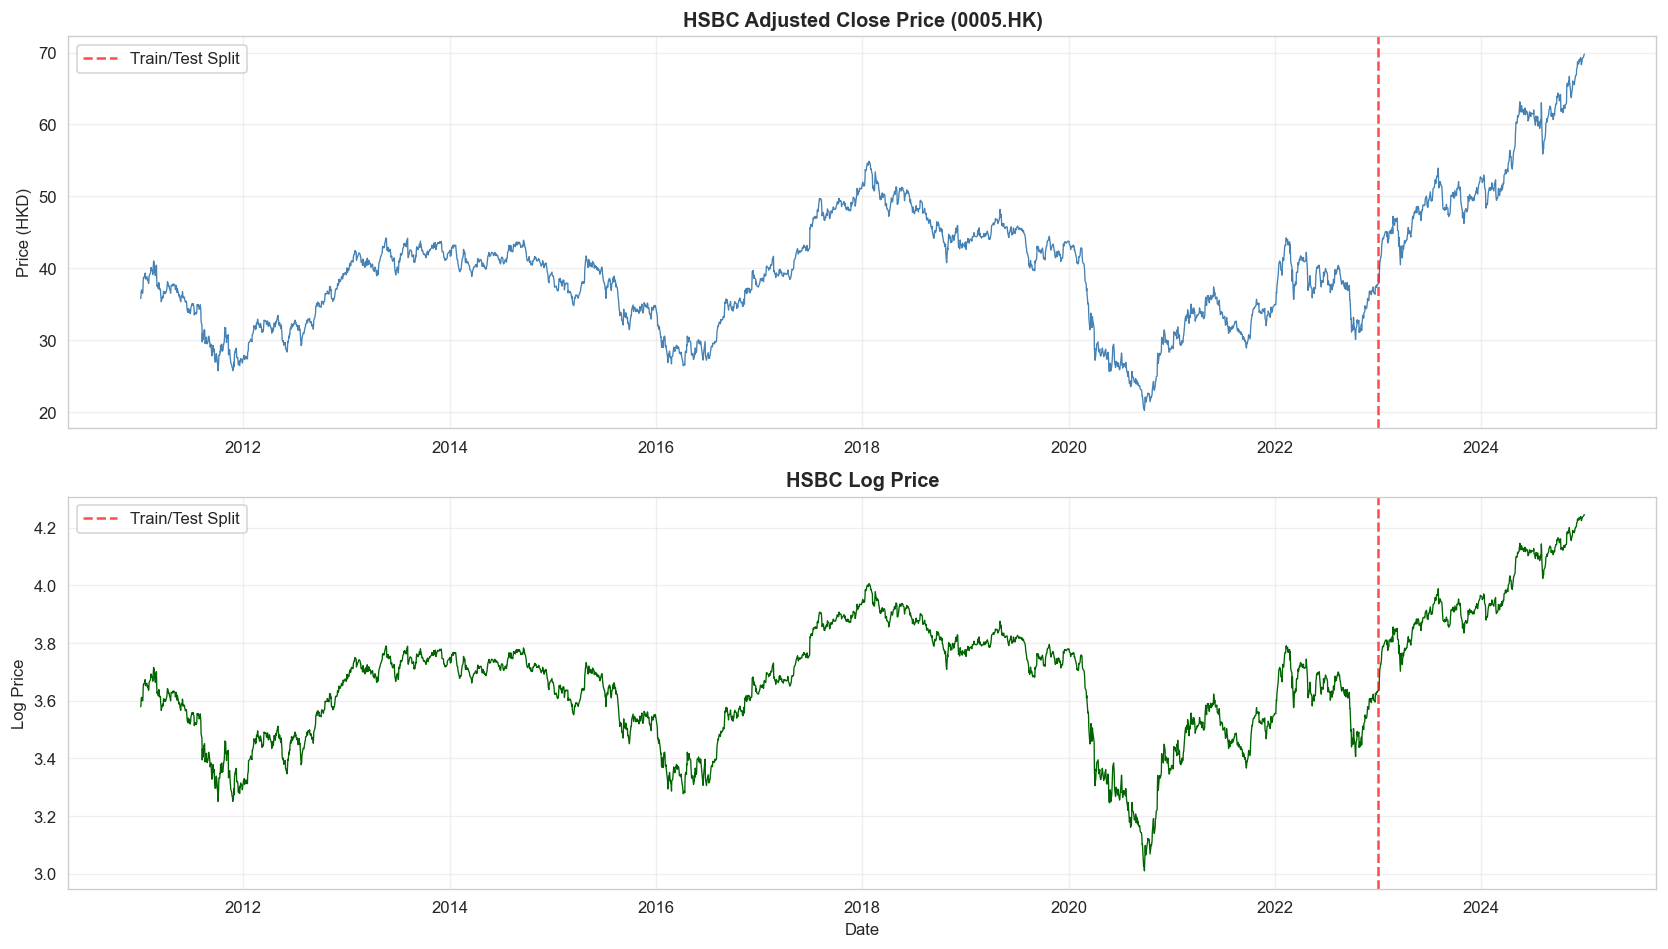
\includegraphics[width=\linewidth]{figures/hsbc_price_logprice.png}
    \caption{HSBC adjusted close price and log price.}
    \label{fig:hsbc_price_logprice}
\end{figure}

\begin{figure}[htbp]
    \centering
    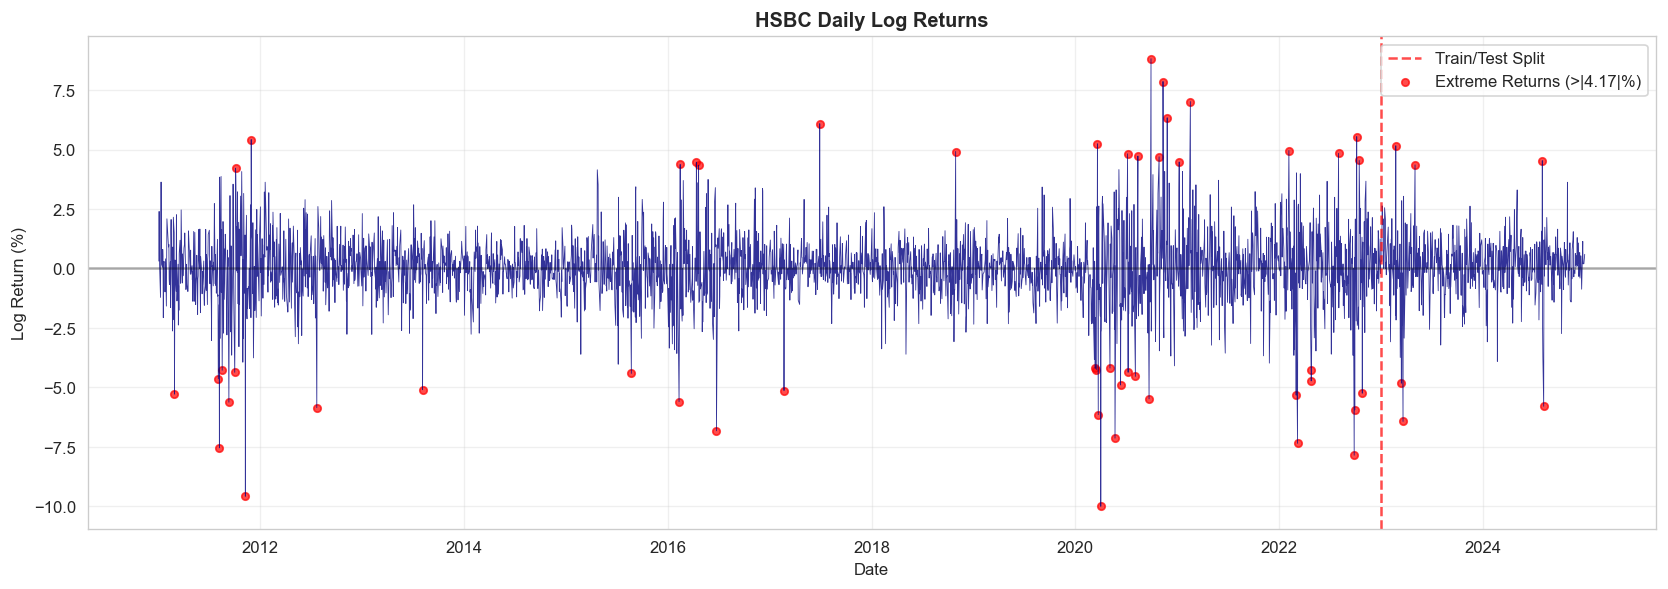
\includegraphics[width=\linewidth]{figures/hsbc_log_returns.png}
    \caption{HSBC daily log returns.}
    \label{fig:hsbc_returns}
\end{figure}

\subsection{Preliminary Statistics}
Table~\ref{tab:hsbc_desc} reports the main descriptive statistics. For the training sample, the average daily return is close to zero at 0.0018\%, while the daily standard deviation is 1.4141\%. Annualising this standard deviation by $\sqrt{252}$ gives an annual volatility of about 22.45\%, which is moderate but economically meaningful for a major banking stock. The minimum and maximum daily returns are -9.9964\% and 8.8193\%, showing that the sample contains large downside and upside shocks.

The return distribution is slightly left-skewed, with skewness equal to -0.2825, and strongly leptokurtic, with excess kurtosis equal to 5.1666. The Jarque--Bera statistic is 3328.2521 with a p-value close to zero, so normality is clearly rejected. These results support the use of volatility models because the HSBC return distribution has heavy tails and time-varying risk.

\begin{table}[htbp]
    \centering
    \caption{Descriptive statistics of HSBC daily log returns.}
    \label{tab:hsbc_desc}
    \begin{tabular}{lrr}
        \hline
        Statistic & Full sample & Training sample \\
        \hline
        Observations & 3445 & 2957 \\
        Mean & 0.0194 & 0.0018 \\
        Standard deviation & 1.3906 & 1.4141 \\
        Minimum & -9.9964 & -9.9964 \\
        Maximum & 8.8193 & 8.8193 \\
        Skewness & -0.3230 & -0.2825 \\
        Excess kurtosis & 5.1105 & 5.1666 \\
        Jarque--Bera statistic & 3808.7425 & 3328.2521 \\
        Jarque--Bera p-value & 0.0000 & 0.0000 \\
        \hline
    \end{tabular}
\end{table}

\subsection{Stationarity and Serial Correlation}
The ADF test confirms the usual financial time-series pattern. The log price is non-stationary, with an ADF statistic of -1.1221 and p-value of 0.7062. In contrast, the log return is strongly stationary, with an ADF statistic of -39.8720 and p-value close to zero. Therefore, the modelling is conducted on daily log returns rather than price levels.

The Ljung--Box test on training returns shows limited but non-negligible serial correlation. The p-values are 0.2872, 0.2144, 0.0714, and 0.0285 at lags 5, 10, 15, and 20 respectively, so the null of no serial correlation is rejected at lag 20. Figure~\ref{fig:hsbc_acf_pacf} further suggests that the mean dynamics are weak but not entirely absent, motivating an ARMA search over low-order specifications.

\begin{figure}[htbp]
    \centering
    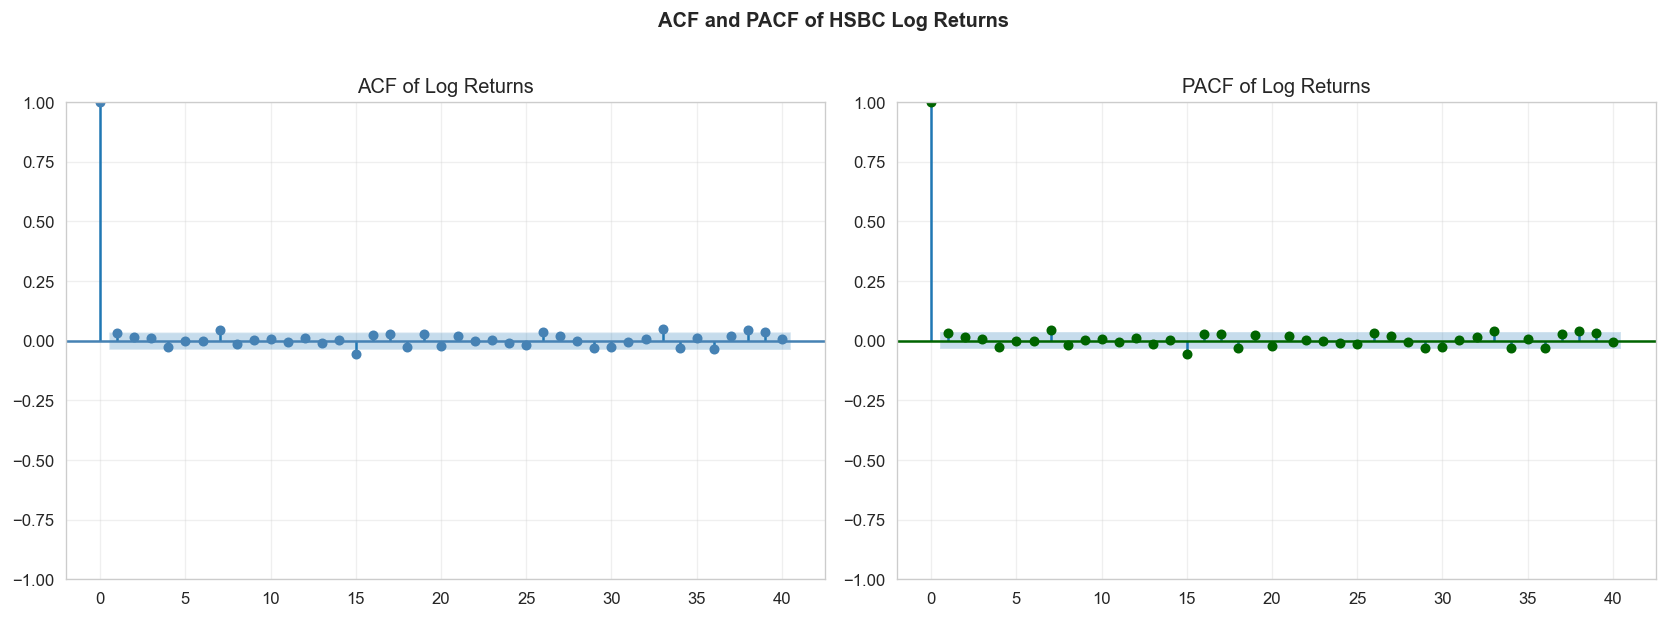
\includegraphics[width=\linewidth]{figures/hsbc_acf_pacf_returns.png}
    \caption{ACF and PACF of HSBC training-period log returns.}
    \label{fig:hsbc_acf_pacf}
\end{figure}

\subsection{ARMA Mean Model}
ARMA candidates with $p,q \leq 2$ are compared using AIC, BIC, and residual Ljung--Box diagnostics. AIC selects ARMA(2,2), while BIC selects the more parsimonious ARMA(1,0). Since the residual Ljung--Box p-value of ARMA(2,2) is the strongest among the candidates and its AIC is materially lower, ARMA(2,2) is used as the preferred mean model.

The fitted ARMA(2,2) model has significant AR and MA terms, but the constant is not significant, which is consistent with the near-zero mean of daily stock returns. The residual Ljung--Box p-values are 0.8896, 0.7040, and 0.4190 at lags 5, 10, and 15, respectively. Thus, the ARMA model removes most linear serial correlation. However, the ARCH-LM statistic is 127.4144 with p-value 0.0000, indicating strong remaining conditional heteroskedasticity. Figure~\ref{fig:hsbc_squared_acf} also shows significant autocorrelation in squared residuals, so a GARCH-type volatility model is required.

\begin{table}[htbp]
    \centering
    \caption{ARMA model selection for HSBC training returns.}
    \label{tab:hsbc_arma}
    \begin{tabular}{lrrr}
        \hline
        Model & AIC & BIC & Residual LB p-value \\
        \hline
        ARMA(0,1) & 10442.8609 & 10460.8367 & 0.4021 \\
        ARMA(1,0) & 10442.7644 & 10460.7402 & 0.4088 \\
        ARMA(2,0) & 10444.0021 & 10467.9698 & 0.4722 \\
        ARMA(2,2) & 10435.5301 & 10471.4817 & 0.7040 \\
        \hline
    \end{tabular}
\end{table}

\begin{figure}[htbp]
    \centering
    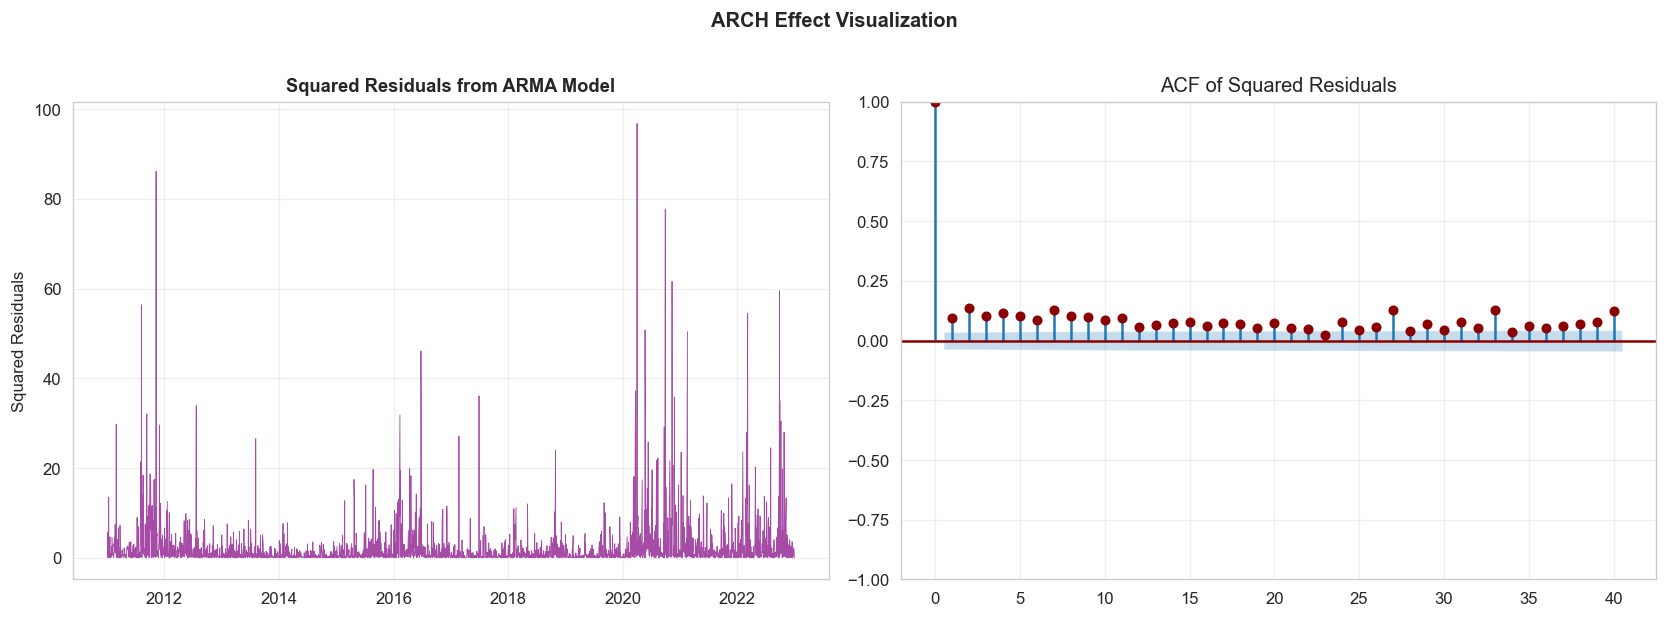
\includegraphics[width=\linewidth]{figures/hsbc_squared_residuals_acf.png}
    \caption{Squared ARMA residuals and their ACF.}
    \label{fig:hsbc_squared_acf}
\end{figure}

\subsection{Volatility Model}
The ARCH evidence is strong. Ljung--Box tests on squared ARMA residuals give statistics of 181.7378, 334.9748, and 418.1917 at lags 5, 10, and 15, with p-values close to zero. This confirms volatility clustering in HSBC returns.

Table~\ref{tab:hsbc_garch} compares GARCH(1,1) and EGARCH(1,1). For GARCH(1,1), the ARCH coefficient is 0.0524 and the GARCH coefficient is 0.9373, producing a persistence measure of 0.9897. This value is close to one, implying that volatility shocks decay slowly. EGARCH(1,1) has a slightly lower AIC of 9842.6454 compared with 9846.0254 for GARCH(1,1), so it is preferred by AIC. However, the estimated asymmetry term is effectively zero in this specification, so there is no strong evidence of a leverage effect for HSBC in this sample.

Figure~\ref{fig:hsbc_condvol} shows that both volatility models capture time-varying risk. Conditional volatility rises sharply during the 2020 Covid-19 period and remains elevated during parts of the 2022 rate-hiking cycle, consistent with the sensitivity of bank stocks to macro-financial shocks and interest-rate expectations.

\begin{table}[htbp]
    \centering
    \caption{GARCH-type model comparison for HSBC.}
    \label{tab:hsbc_garch}
    \begin{tabular}{lrr}
        \hline
        Statistic & GARCH(1,1) & EGARCH(1,1) \\
        \hline
        Alpha & 0.0524 & N/A \\
        Beta & 0.9373 & 0.9870 \\
        Persistence & 0.9897 & 0.9870 \\
        Asymmetry & N/A & 0.0000 \\
        AIC & 9846.0254 & 9842.6454 \\
        BIC & 9869.9931 & 9866.6131 \\
        \hline
    \end{tabular}
\end{table}

\begin{figure}[htbp]
    \centering
    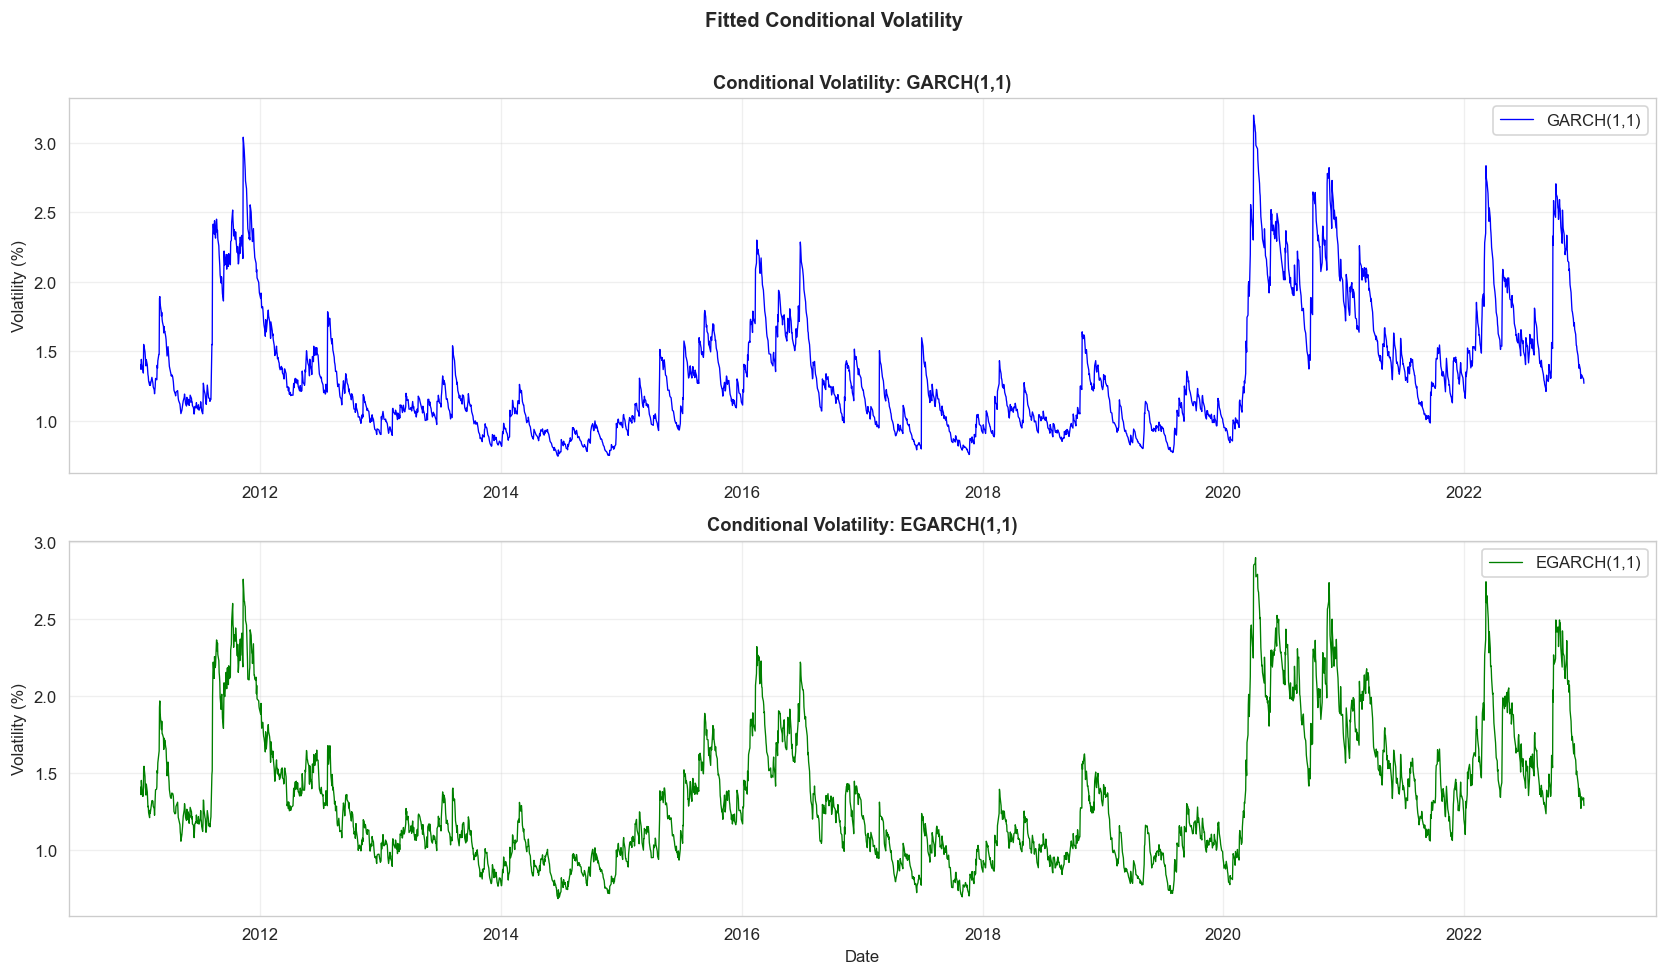
\includegraphics[width=\linewidth]{figures/hsbc_conditional_volatility.png}
    \caption{Fitted conditional volatility from GARCH(1,1) and EGARCH(1,1).}
    \label{fig:hsbc_condvol}
\end{figure}

\subsection{Forecasting}
Forecasting is evaluated on the 2023--2024 test period using rolling one-step-ahead forecasts. The ARMA benchmark uses the selected ARMA(2,2) mean model, while the volatility-based model uses an AR(1)-GARCH(1,1) recursion for the conditional mean and variance.

Table~\ref{tab:hsbc_forecast} shows that AR(1)-GARCH(1,1) performs slightly better than ARMA in RMSE and MAE. Its RMSE is 1.2399 compared with 1.2560 for ARMA, and its MAE is 0.8846 compared with 0.8978. Directional accuracy also improves from 50.8197\% to 52.0492\%. The improvement is small, which is consistent with the general difficulty of predicting daily stock returns. The main value of the GARCH model is therefore not a large gain in mean-return prediction, but a more informative forecast of conditional volatility and risk.

\begin{table}[htbp]
    \centering
    \caption{Forecasting performance on the 2023--2024 test set.}
    \label{tab:hsbc_forecast}
    \begin{tabular}{lrr}
        \hline
        Metric & ARMA rolling 1-step & AR(1)-GARCH rolling 1-step \\
        \hline
        RMSE & 1.2560 & 1.2399 \\
        MAE & 0.8978 & 0.8846 \\
        sMAPE (\%) & 176.4755 & 181.5674 \\
        Directional accuracy (\%) & 50.8197 & 52.0492 \\
        \hline
    \end{tabular}
\end{table}

\begin{figure}[htbp]
    \centering
    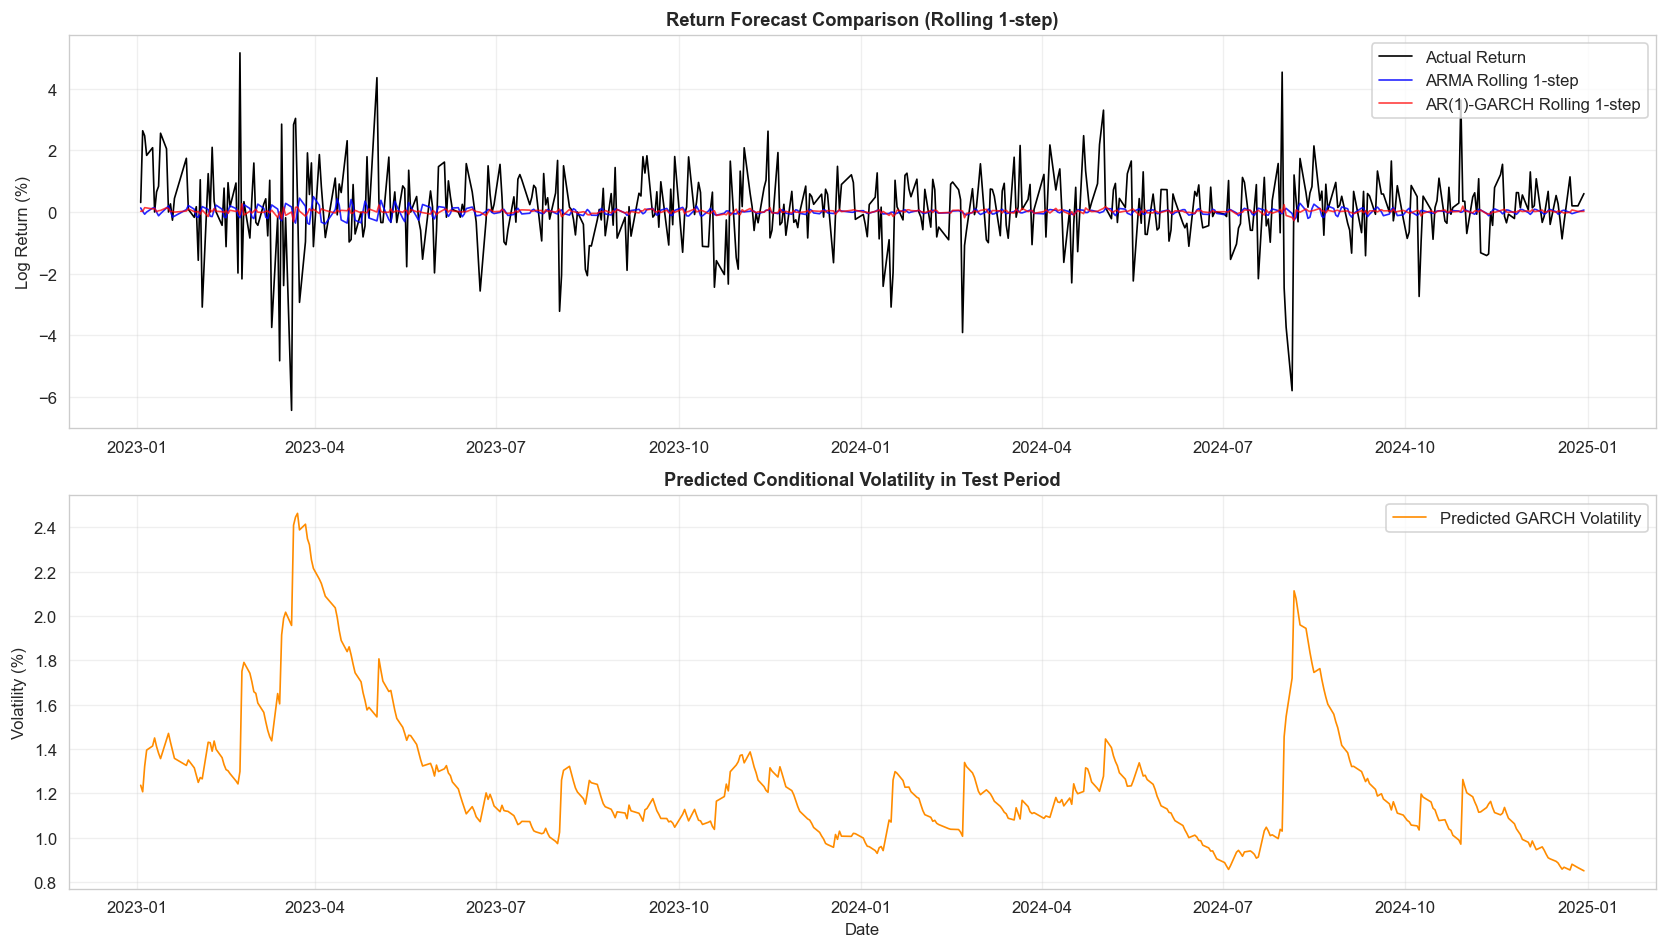
\includegraphics[width=\linewidth]{figures/hsbc_forecast_comparison.png}
    \caption{Rolling one-step return forecast and predicted conditional volatility.}
    \label{fig:hsbc_forecast}
\end{figure}

\subsection{Individual Conclusion -- HSBC}
HSBC's daily return process is stationary, close to zero mean, and only weakly predictable in the mean. The preferred ARMA(2,2) model removes most linear autocorrelation, but the residuals retain strong ARCH effects. This indicates that HSBC is better characterised as a stock with time-varying risk rather than a stock with strong daily return predictability.

The volatility results are economically important. The GARCH persistence of 0.9897 implies that shocks to HSBC's volatility are highly persistent, which is consistent with a banking stock exposed to global risk sentiment, monetary policy, and financial-cycle conditions. EGARCH(1,1) has the best AIC, but the leverage term is not economically meaningful in the fitted model, so the evidence for asymmetric volatility is weak. In forecasting, AR(1)-GARCH(1,1) gives a modest improvement over ARMA, with the best directional accuracy around 52\%. Overall, HSBC is more useful for modelling and forecasting conditional volatility than for generating strong short-horizon return forecasts.

% =====================================================================
\section{AIA Group (1299.HK)}
\label{sec:aia}

\subsection{Data Description}
AIA Group Limited is Asia's largest independent publicly listed pan-Asian
life insurance group, listed on the Hong Kong Stock Exchange.  As a
blue-chip financial stock with significant weight in the Hang Seng Index,
AIA is sensitive to interest rates, equity market performance, insurance
demand cycles and regional macroeconomic conditions across 18
Asia-Pacific markets.  Paired with HSBC, AIA represents the insurance
sub-sector within financials: both are exposed to the rate cycle, but
AIA's business mix tilts toward wealth management and protection products
rather than lending.

The sample period is 2011-01-03 to 2024-12-30, yielding $3{,}446$ trading
days ($3{,}445$ usable log-return observations).  The price series
exhibits a long-term upward trend from approximately HKD~18 in 2011 to
HKD~55 by end-2024, interrupted by two major drawdowns: the 2015--2016
China market turmoil and the 2020 COVID-19 pandemic crash.

\begin{figure}[H]
\centering
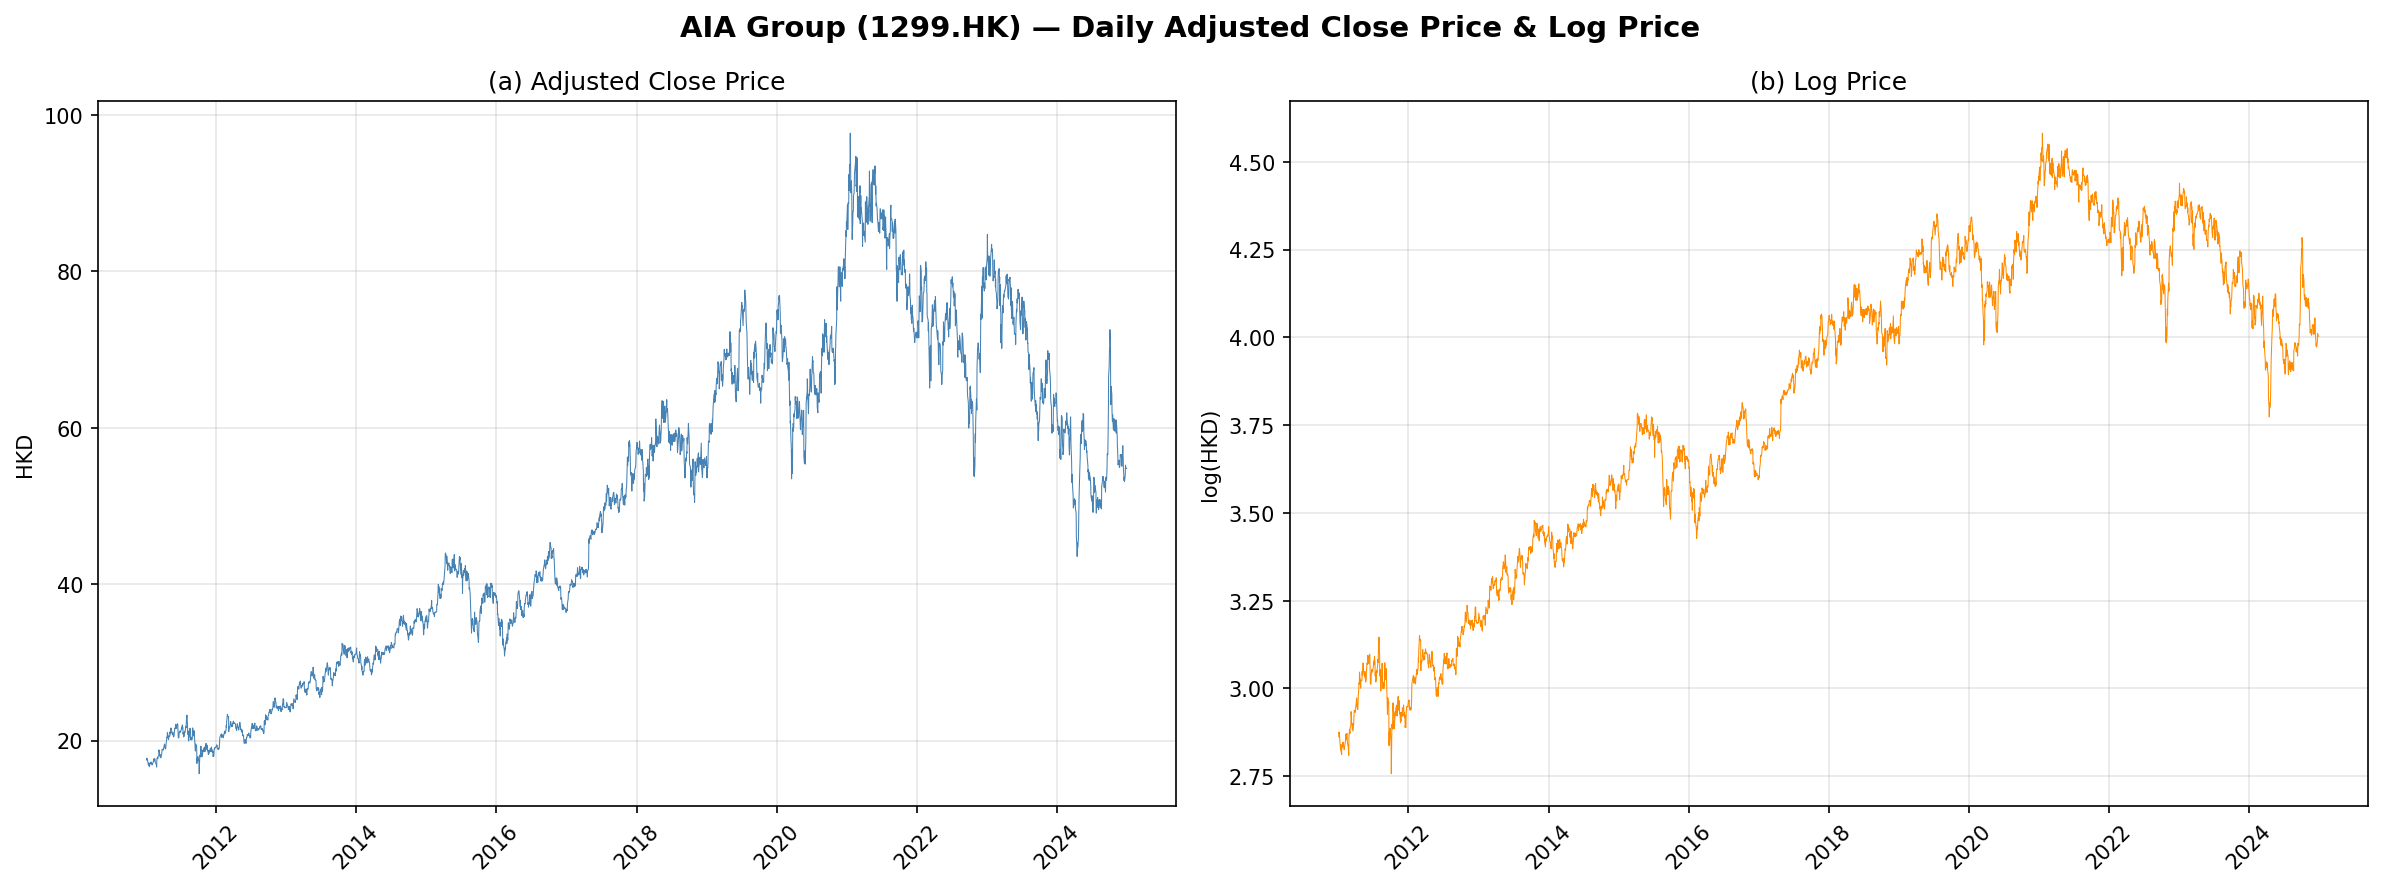
\includegraphics[width=0.95\linewidth]{aia_figure1_price_and_log_price.png}
\caption{AIA price and log price (2011--2024).}
\label{fig:aia-price}
\end{figure}

\begin{figure}[H]
\centering
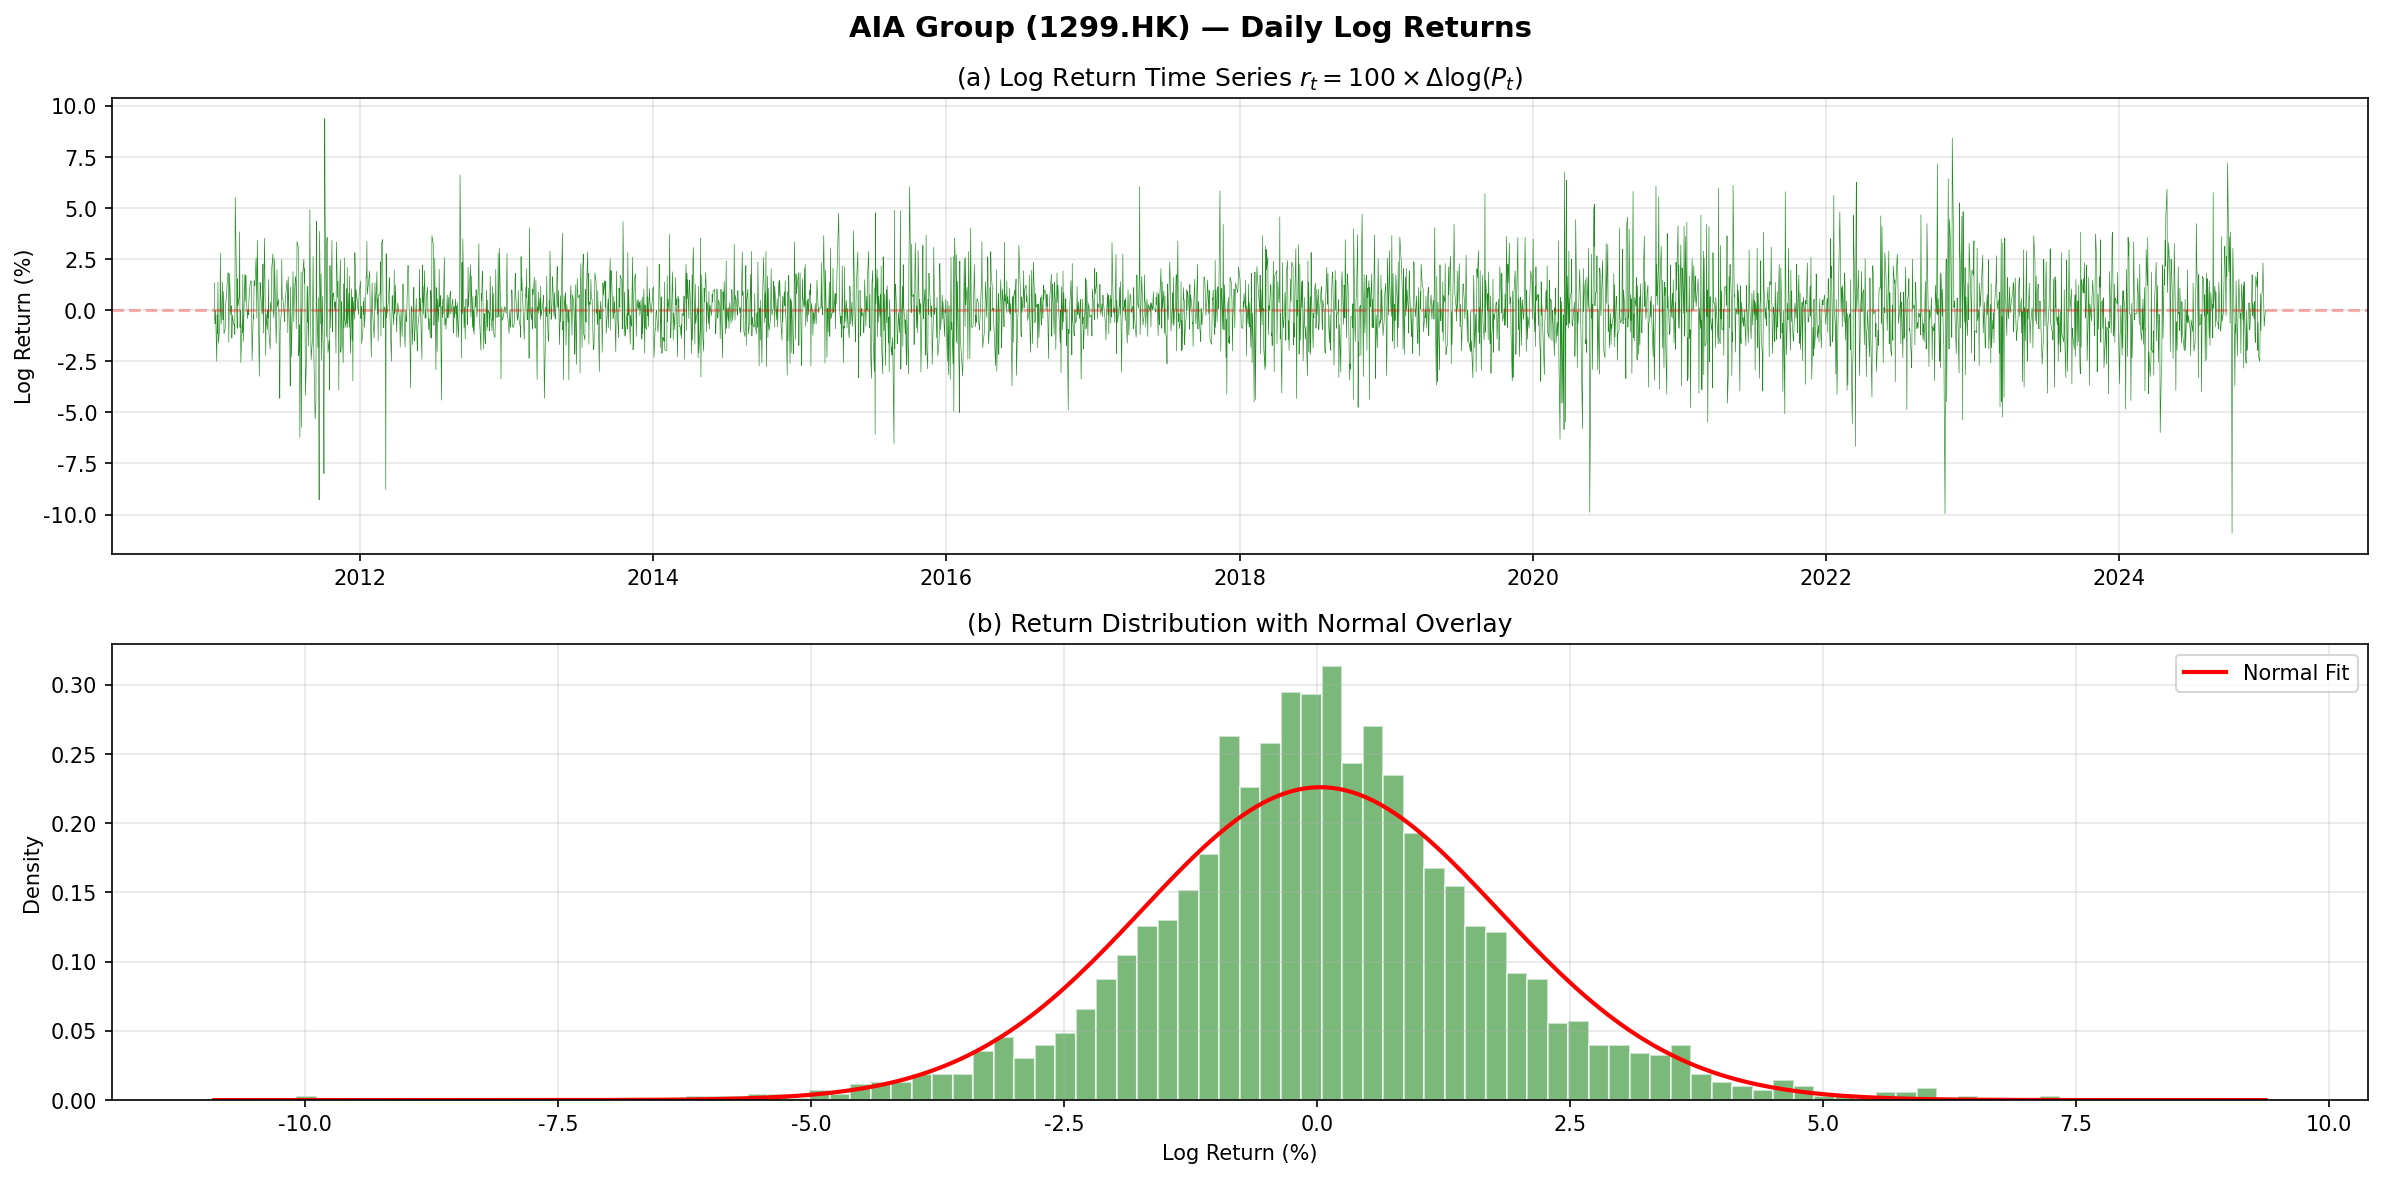
\includegraphics[width=0.95\linewidth]{aia_figure2_log_return_plot.png}
\caption{AIA daily log return (\%) (2011--2024).  Volatility clustering is
clearly visible, with extended calm periods (2012--2014, 2017--2019)
alternating with elevated-volatility episodes (2015--2016 China sell-off,
COVID-19 crash in March~2020, and the 2022 rate-hike cycle).}
\label{fig:aia-return}
\end{figure}

\subsection{Preliminary Statistics}
Mean daily log return over the training period (2011--2022) is
$0.0516\%$ and the standard deviation is $1.7350\%$, placing AIA between
HSBC (1.41\%) and Tencent (2.18\%) in unconditional volatility.  The
daily return ranges from $-9.96\%$ to $+9.38\%$, broadly symmetric around
the mean.  Skewness is $-0.052$ (near zero) and excess kurtosis is
$2.82$, well above the Gaussian benchmark.  The Jarque--Bera statistic is
$974.53$ with $p \approx 0$, firmly rejecting normality.  The heavy tails
and the rejection of normality justify the use of GARCH-type volatility
models rather than a homoskedastic Gaussian framework.

\begin{table}[H]
\centering
\small
\begin{tabular}{rrrrrrrrr}
\toprule
count & mean & sd & min & max & skewness & kurtosis & jarque\_bera & jb\_pvalue \\
\midrule
2958 & 0.0516 & 1.7350 & -9.9565 & 9.3759 & -0.0516 & 5.8173 & 974.5257 & 0.0000 \\
\bottomrule
\end{tabular}
\caption{AIA descriptive statistics (daily log return, \%).}
\label{tab:aia-desc}
\end{table}

\subsection{Stationarity and Serial Correlation}
ADF on log price gives $-1.44$ ($p = 0.56$): the unit-root null cannot
be rejected, confirming that the price level is non-stationary.  ADF on
log return gives $-41.21$ ($p < 0.001$): returns are strongly stationary.

Ljung--Box on raw returns at lag~6 is significant ($p = 0.0195$),
indicating modest short-horizon serial dependence that warrants ARMA
modeling.  The LB test on \emph{squared} returns, however, is
overwhelmingly significant at every horizon -- the ARCH-LM test on
ARMA residuals yields LM~$=172.41$ ($p \approx 0$).  Volatility
clustering is therefore the dominant time-series feature of AIA returns.

\begin{figure}[H]
\centering
\begin{subfigure}{0.49\linewidth}
  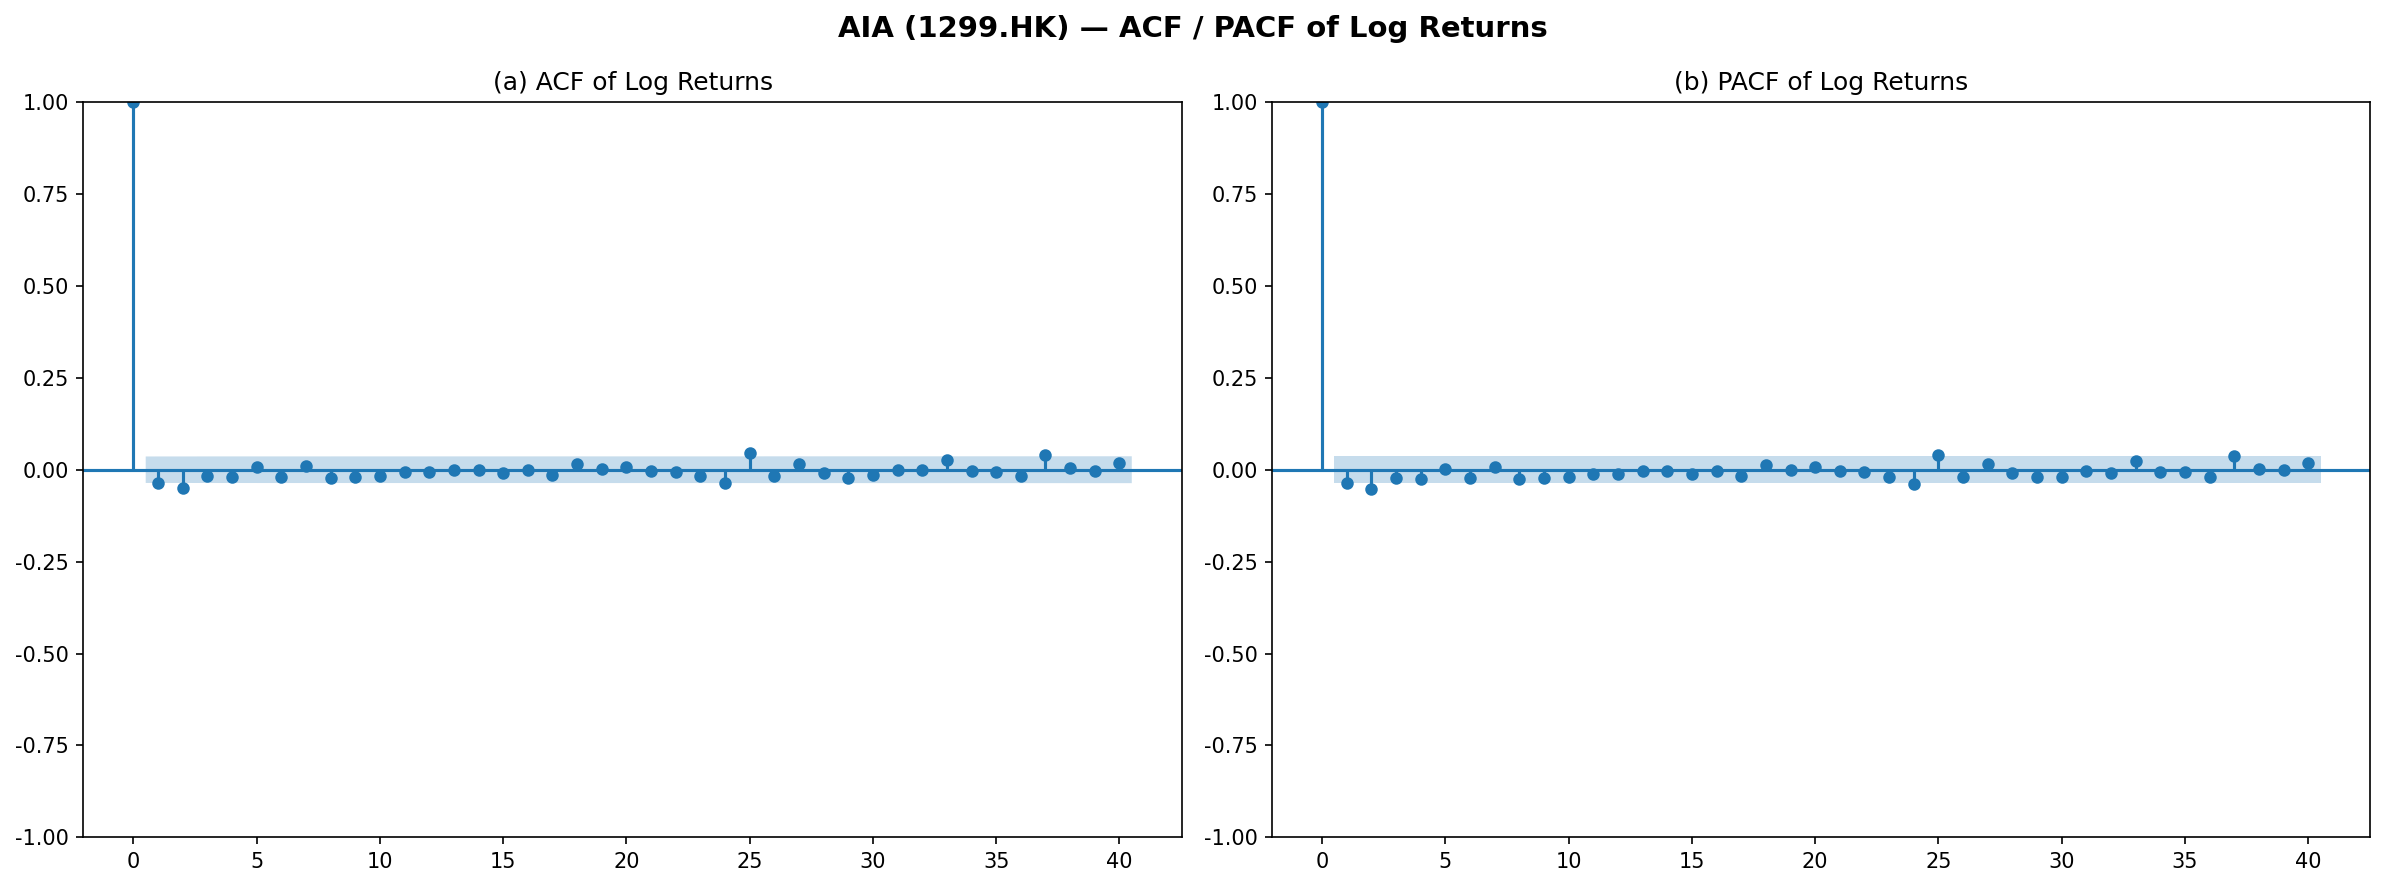
\includegraphics[width=\linewidth]{aia_figure3_acf_pacf_returns.png}
  \caption{ACF/PACF of returns}
\end{subfigure}\hfill
\begin{subfigure}{0.49\linewidth}
  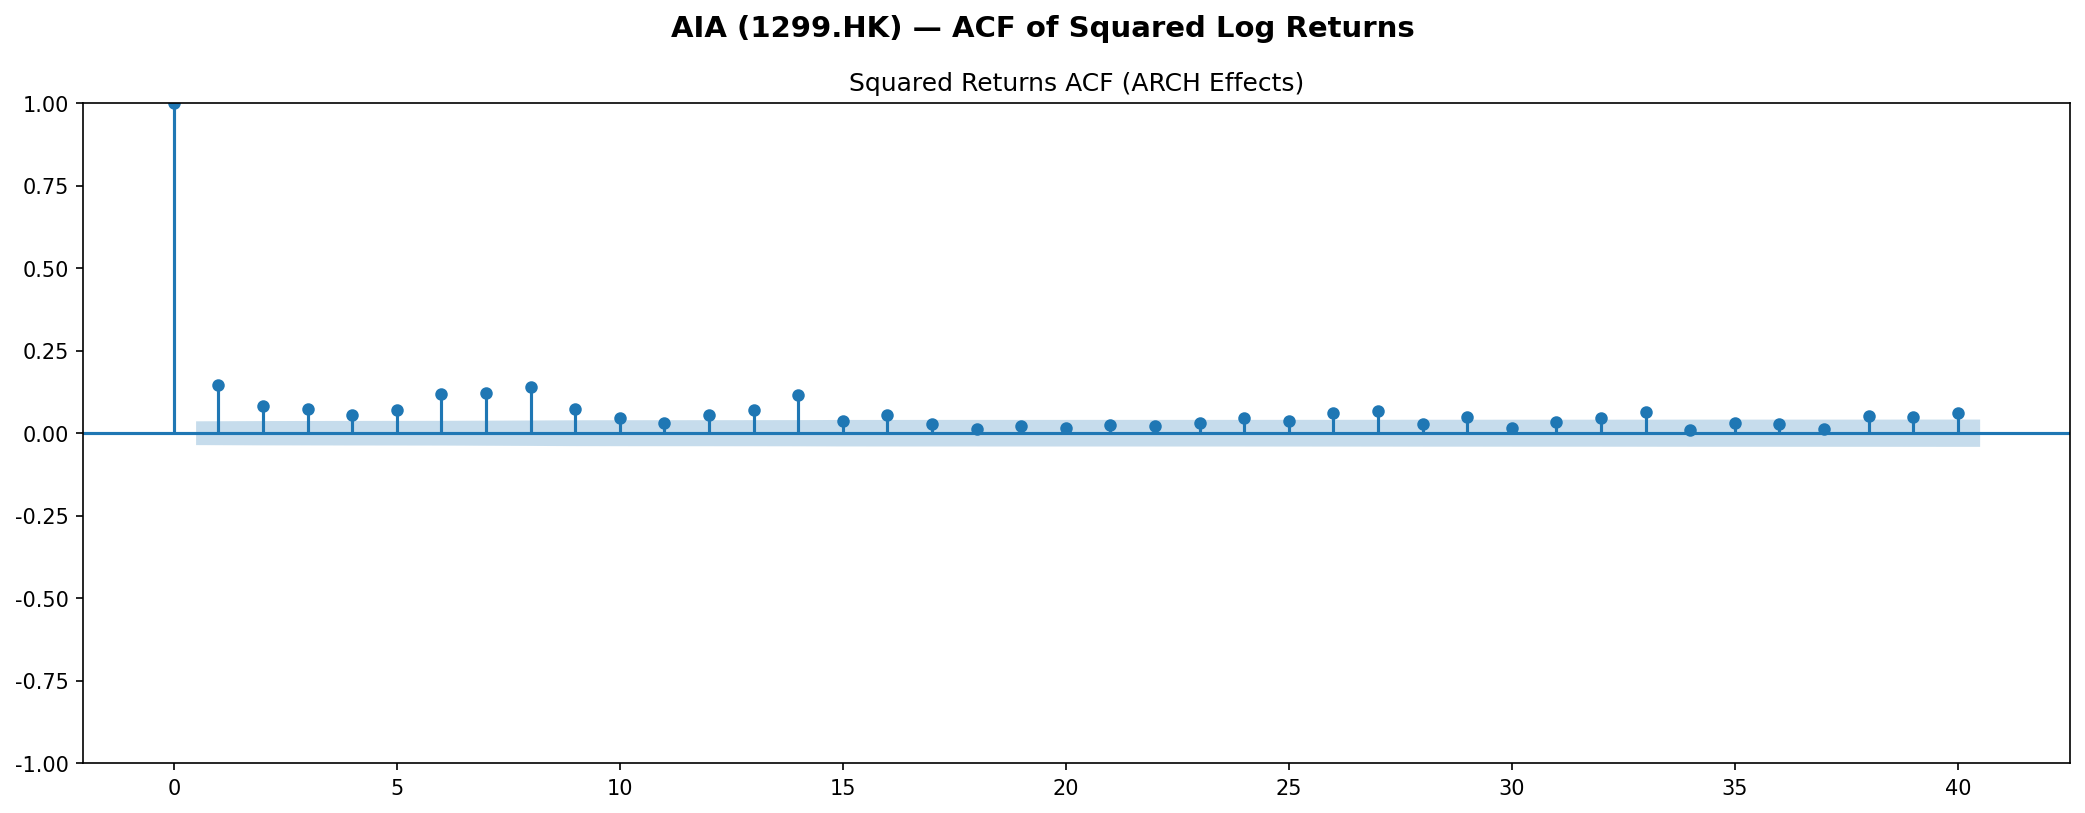
\includegraphics[width=\linewidth]{aia_figure4_acf_squared_returns.png}
  \caption{ACF of squared returns}
\end{subfigure}
\caption{AIA serial-correlation diagnostics.  The squared-return ACF
confirms strong volatility clustering.}
\label{fig:aia-acf}
\end{figure}

\begin{table}[H]
\centering
\small
\begin{tabular}{llrrr}
\toprule
series & test & lag & stat & pvalue \\
\midrule
log\_price           & ADF        & auto & $-1.4373$  & $0.5643$ \\
log\_return          & ADF        & auto & $-41.2054$ & $0.0000$ \\
log\_return          & Ljung--Box & 10   & $15.0987$  & $0.0195$ \\
squared\_return      & Ljung--Box & 10   & $304.9241$ & $0.0000$ \\
log\_return          & Ljung--Box & 20   & $24.3000$  & $0.0350$ \\
squared\_return      & Ljung--Box & 20   & $500.0000$ & $0.0000$ \\
\bottomrule
\end{tabular}
\caption{AIA stationarity tests.}
\label{tab:aia-stat}
\end{table}

\subsection{ARMA Mean Model}
We searched ARMA$(p,q)$ over $p,q \in \{0,1,2,3\}$ using AIC and BIC.
The preferred specification is \textbf{ARMA(1,1)} (AIC~$=11640.13$,
BIC~$=11664.10$, residual LB(12) $p = 0.717$).  The modest
autoregressive and moving-average terms capture the short-horizon serial
dependence visible in the ACF/PACF, while producing residuals that are
approximately white noise in the mean.  This is consistent with
semi-strong market efficiency: AIA returns are weakly predictable in the
short term, but the economic magnitude is small.

Residual diagnostics confirm that the ARMA(1,1) specification adequately
captures the conditional mean.  However, the ARCH-LM test on the ARMA
residuals is highly significant (LM~$=172.41$, $p \approx 0$), and the
Ljung--Box test on squared residuals rejects independence at all lags.
Conditional heteroskedasticity remains, and a GARCH-type variance model
is therefore essential.

\begin{table}[H]
\centering
\small
\begin{tabular}{lrrrrr}
\toprule
model & p & q & AIC & BIC & LB(12) $p$ \\
\midrule
ARMA(1,1) & 1 & 1 & 11640.13 & 11664.10 & 0.7174 \\
ARMA(2,2) & 2 & 2 & 11641.21 & 11677.17 & 0.7466 \\
ARMA(1,2) & 1 & 2 & 11642.13 & 11672.09 & 0.6172 \\
ARMA(2,1) & 2 & 1 & 11642.13 & 11672.09 & 0.6170 \\
ARMA(4,2) & 4 & 2 & 11642.24 & 11690.17 & 0.3131 \\
ARMA(3,3) & 3 & 3 & 11643.18 & 11691.12 & 0.2476 \\
ARMA(2,3) & 2 & 3 & 11643.41 & 11685.35 & 0.7208 \\
ARMA(3,2) & 3 & 2 & 11643.47 & 11685.41 & 0.7085 \\
\bottomrule
\end{tabular}
\caption{AIA ARMA candidate ranking.  ARMA(1,1) is selected by both AIC and BIC.}
\label{tab:aia-arma}
\end{table}

\subsection{Volatility Model}
Three GARCH-family specifications are estimated on the training set with
an AR(1) mean equation: GARCH(1,1), EGARCH(1,1), and GJR-GARCH(1,1).
By AIC the preferred specification is \textbf{GJR-GARCH(1,1)}
(AIC~$=11396.06$), which explicitly models the leverage effect -- the
tendency for negative returns to increase future volatility more than
positive returns of equal magnitude.

The GJR-GARCH(1,1) estimates are: $\omega = 0.076$, $\alpha_1 = 0.021$,
$\beta_1 = 0.931$, and $\gamma_1 = 0.0453$.  The volatility persistence
$\alpha_1 + \beta_1 = 0.952$ implies a half-life of approximately 29
trading days ($\approx 0.1$ years).  The positive and significant
$\gamma_1$ confirms the leverage effect: bad news (price drops)
disproportionately amplifies future AIA volatility, consistent with the
``fear premium'' observed in financial stocks where capital-adequacy
concerns amplify downside risk.

\begin{figure}[H]
\centering
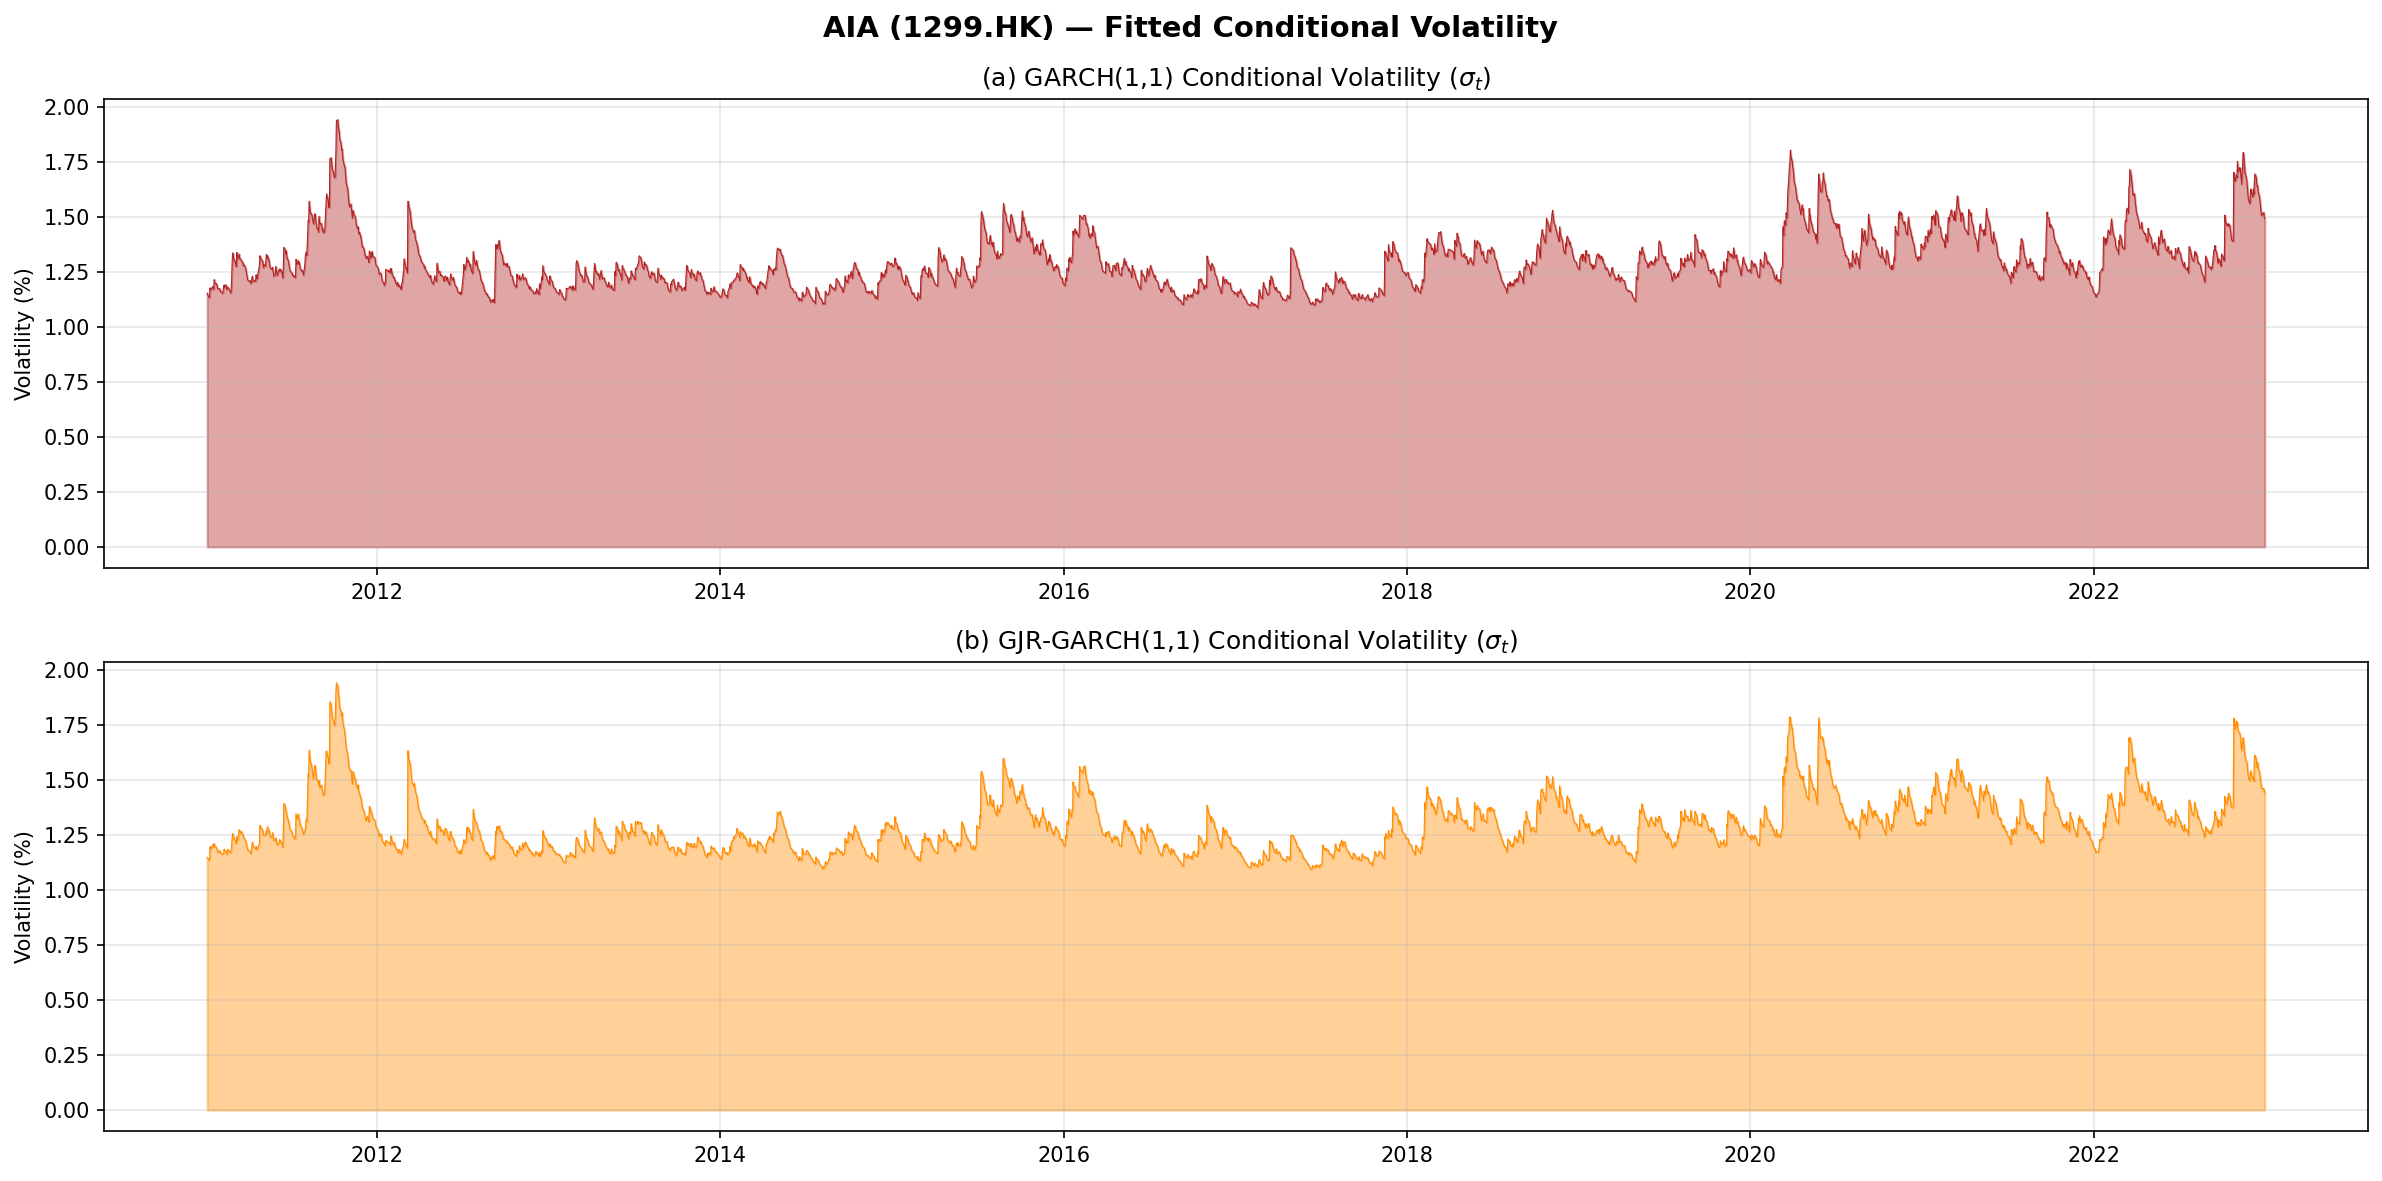
\includegraphics[width=0.95\linewidth]{aia_figure5_conditional_volatility.png}
\caption{AIA fitted conditional volatility (GJR-GARCH(1,1)).  Volatility
spikes align with the 2015--2016 China sell-off, the COVID-19 crash
(March~2020), and the 2022 rate-hike cycle.}
\label{fig:aia-vol}
\end{figure}

\begin{table}[H]
\centering
\small
\begin{tabular}{lrrrrrrr}
\toprule
model & AIC & BIC & $\omega$ & $\alpha_1$ & $\beta_1$ & $\gamma_1$ & $\alpha_1+\beta_1$ \\
\midrule
GJR-GARCH(1,1) & 11396.06 & 11426.02 & 0.0762 & 0.0213 & 0.9307 & 0.0453 & 0.9520 \\
EGARCH(1,1)   & 11409.09 & 11433.06 & 0.0272 & 0.1087 & 0.9794 & --    & 0.9794 \\
GARCH(1,1)    & 11410.07 & 11434.04 & 0.0720 & 0.0486 & 0.9277 & --    & 0.9763 \\
\bottomrule
\end{tabular}
\caption{AIA GARCH-family model comparison.  GJR-GARCH(1,1) is preferred by AIC.}
\label{tab:aia-garch}
\end{table}

\subsection{Forecasting}
Out-of-sample forecasting is conducted on the 2023--2024 test window
($488$ trading days) using a rolling one-step-ahead framework.  Two
specifications are compared: ARMA(1,1) and GJR-GARCH(1,1)-AR(1), both
evaluated on the return scale (log return in \%).

The GJR-GARCH(1,1)-AR(1) model achieves RMSE~$=1.9396\%$ and
MAE~$=1.44\%$, marginally better than the ARMA-only baseline
(RMSE~$=1.9447\%$, MAE~$=1.45\%$).  Directional accuracy is
$46.31\%$ for GJR-GARCH and $48.77\%$ for ARMA -- both below
$50\%$ and statistically indistinguishable from a coin toss.  This
pattern is consistent across all four stocks: GARCH models improve
the description of \emph{conditional variance} but do not materially
improve \emph{directional} return forecasts.  The return-scale forecasts
are plotted in Figure~\ref{fig:aia-fc-ret}.

On the price scale, all three models (ARMA, GJR-GARCH-AR, ARIMA)
produce RMSEs close to $1.24$~HKD, as shown in
Figure~\ref{fig:aia-fc}.  The price-level forecasts benefit from
one-step re-anchoring ($P_{t+1} = P_t \times \exp(\hat{r}_{t+1}/100)$),
which prevents error accumulation and keeps all models nearly
indistinguishable in RMSE.

The return-scale RMSE of approximately $1.94\%$ is comparable to
those reported by the other group members (HSBC: $\approx 1.24\%$,
CLP: $\approx 1.13\%$, Tencent: $\approx 2.07\%$), and the relative
magnitudes align with the unconditional volatility ordering across
sectors.

\begin{figure}[H]
\centering
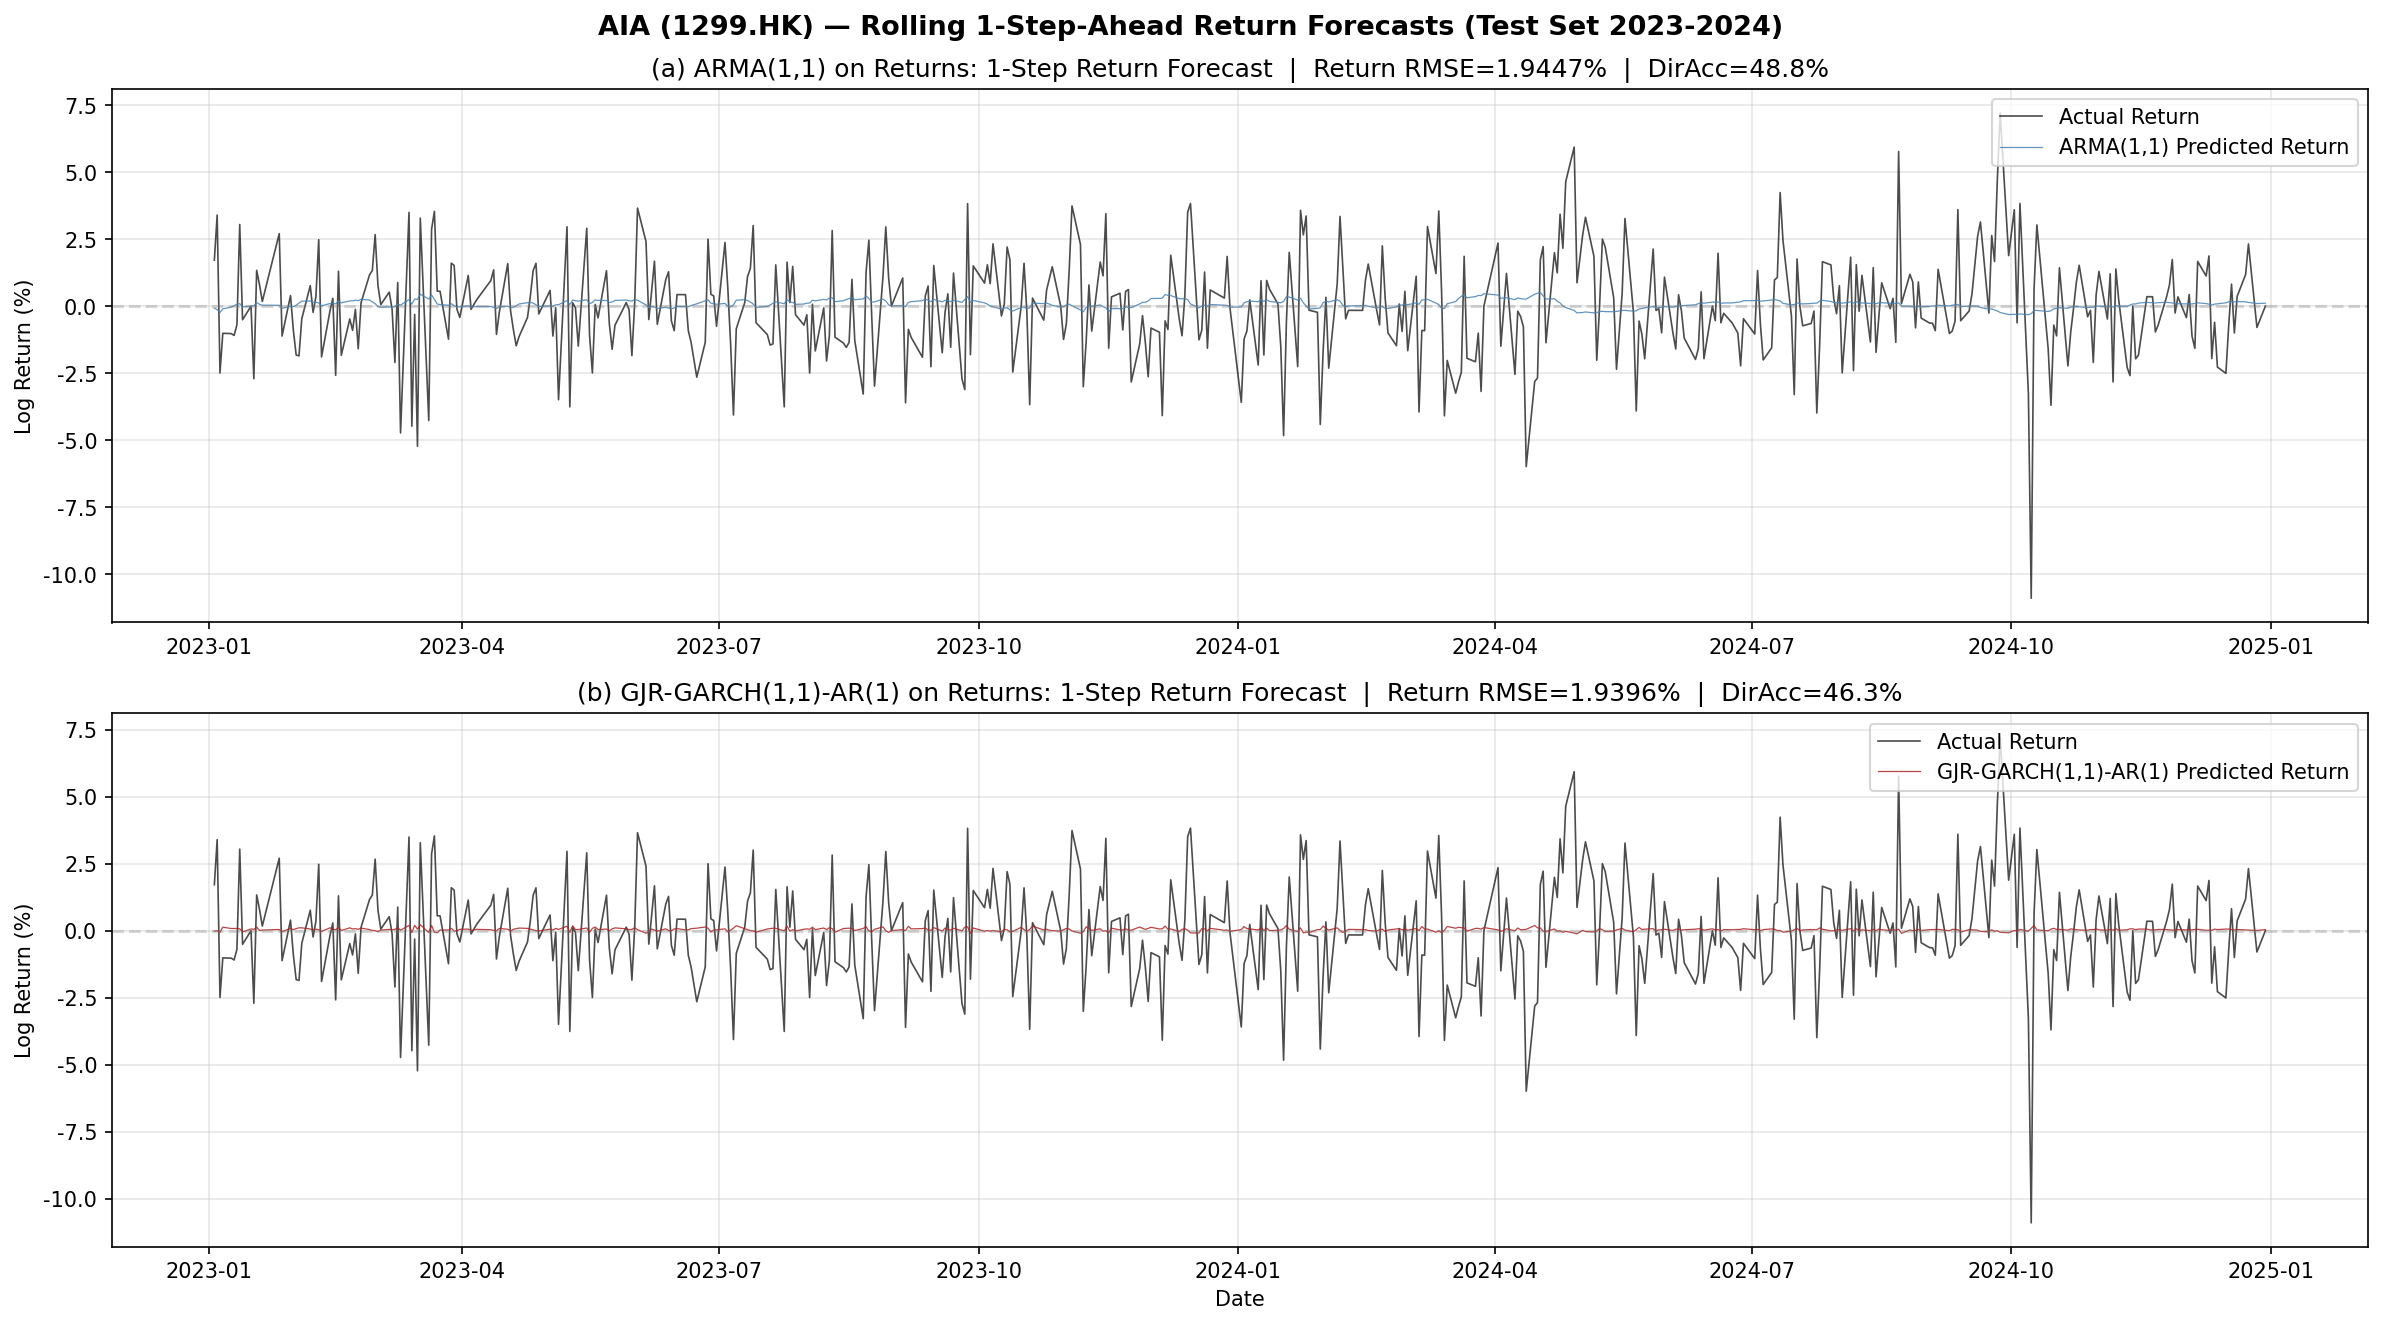
\includegraphics[width=0.95\linewidth]{aia_figure6_return_forecast.png}
\caption{AIA rolling one-step-ahead return forecast vs actual (2023--2024).
Top panel: ARMA(1,1).  Bottom panel: GJR-GARCH(1,1)-AR(1).  Both panels are
on the return scale (\%), providing the return-scale counterpart to
Figure~\ref{fig:aia-fc} for cross-group comparison.}
\label{fig:aia-fc-ret}
\end{figure}

\begin{figure}[H]
\centering
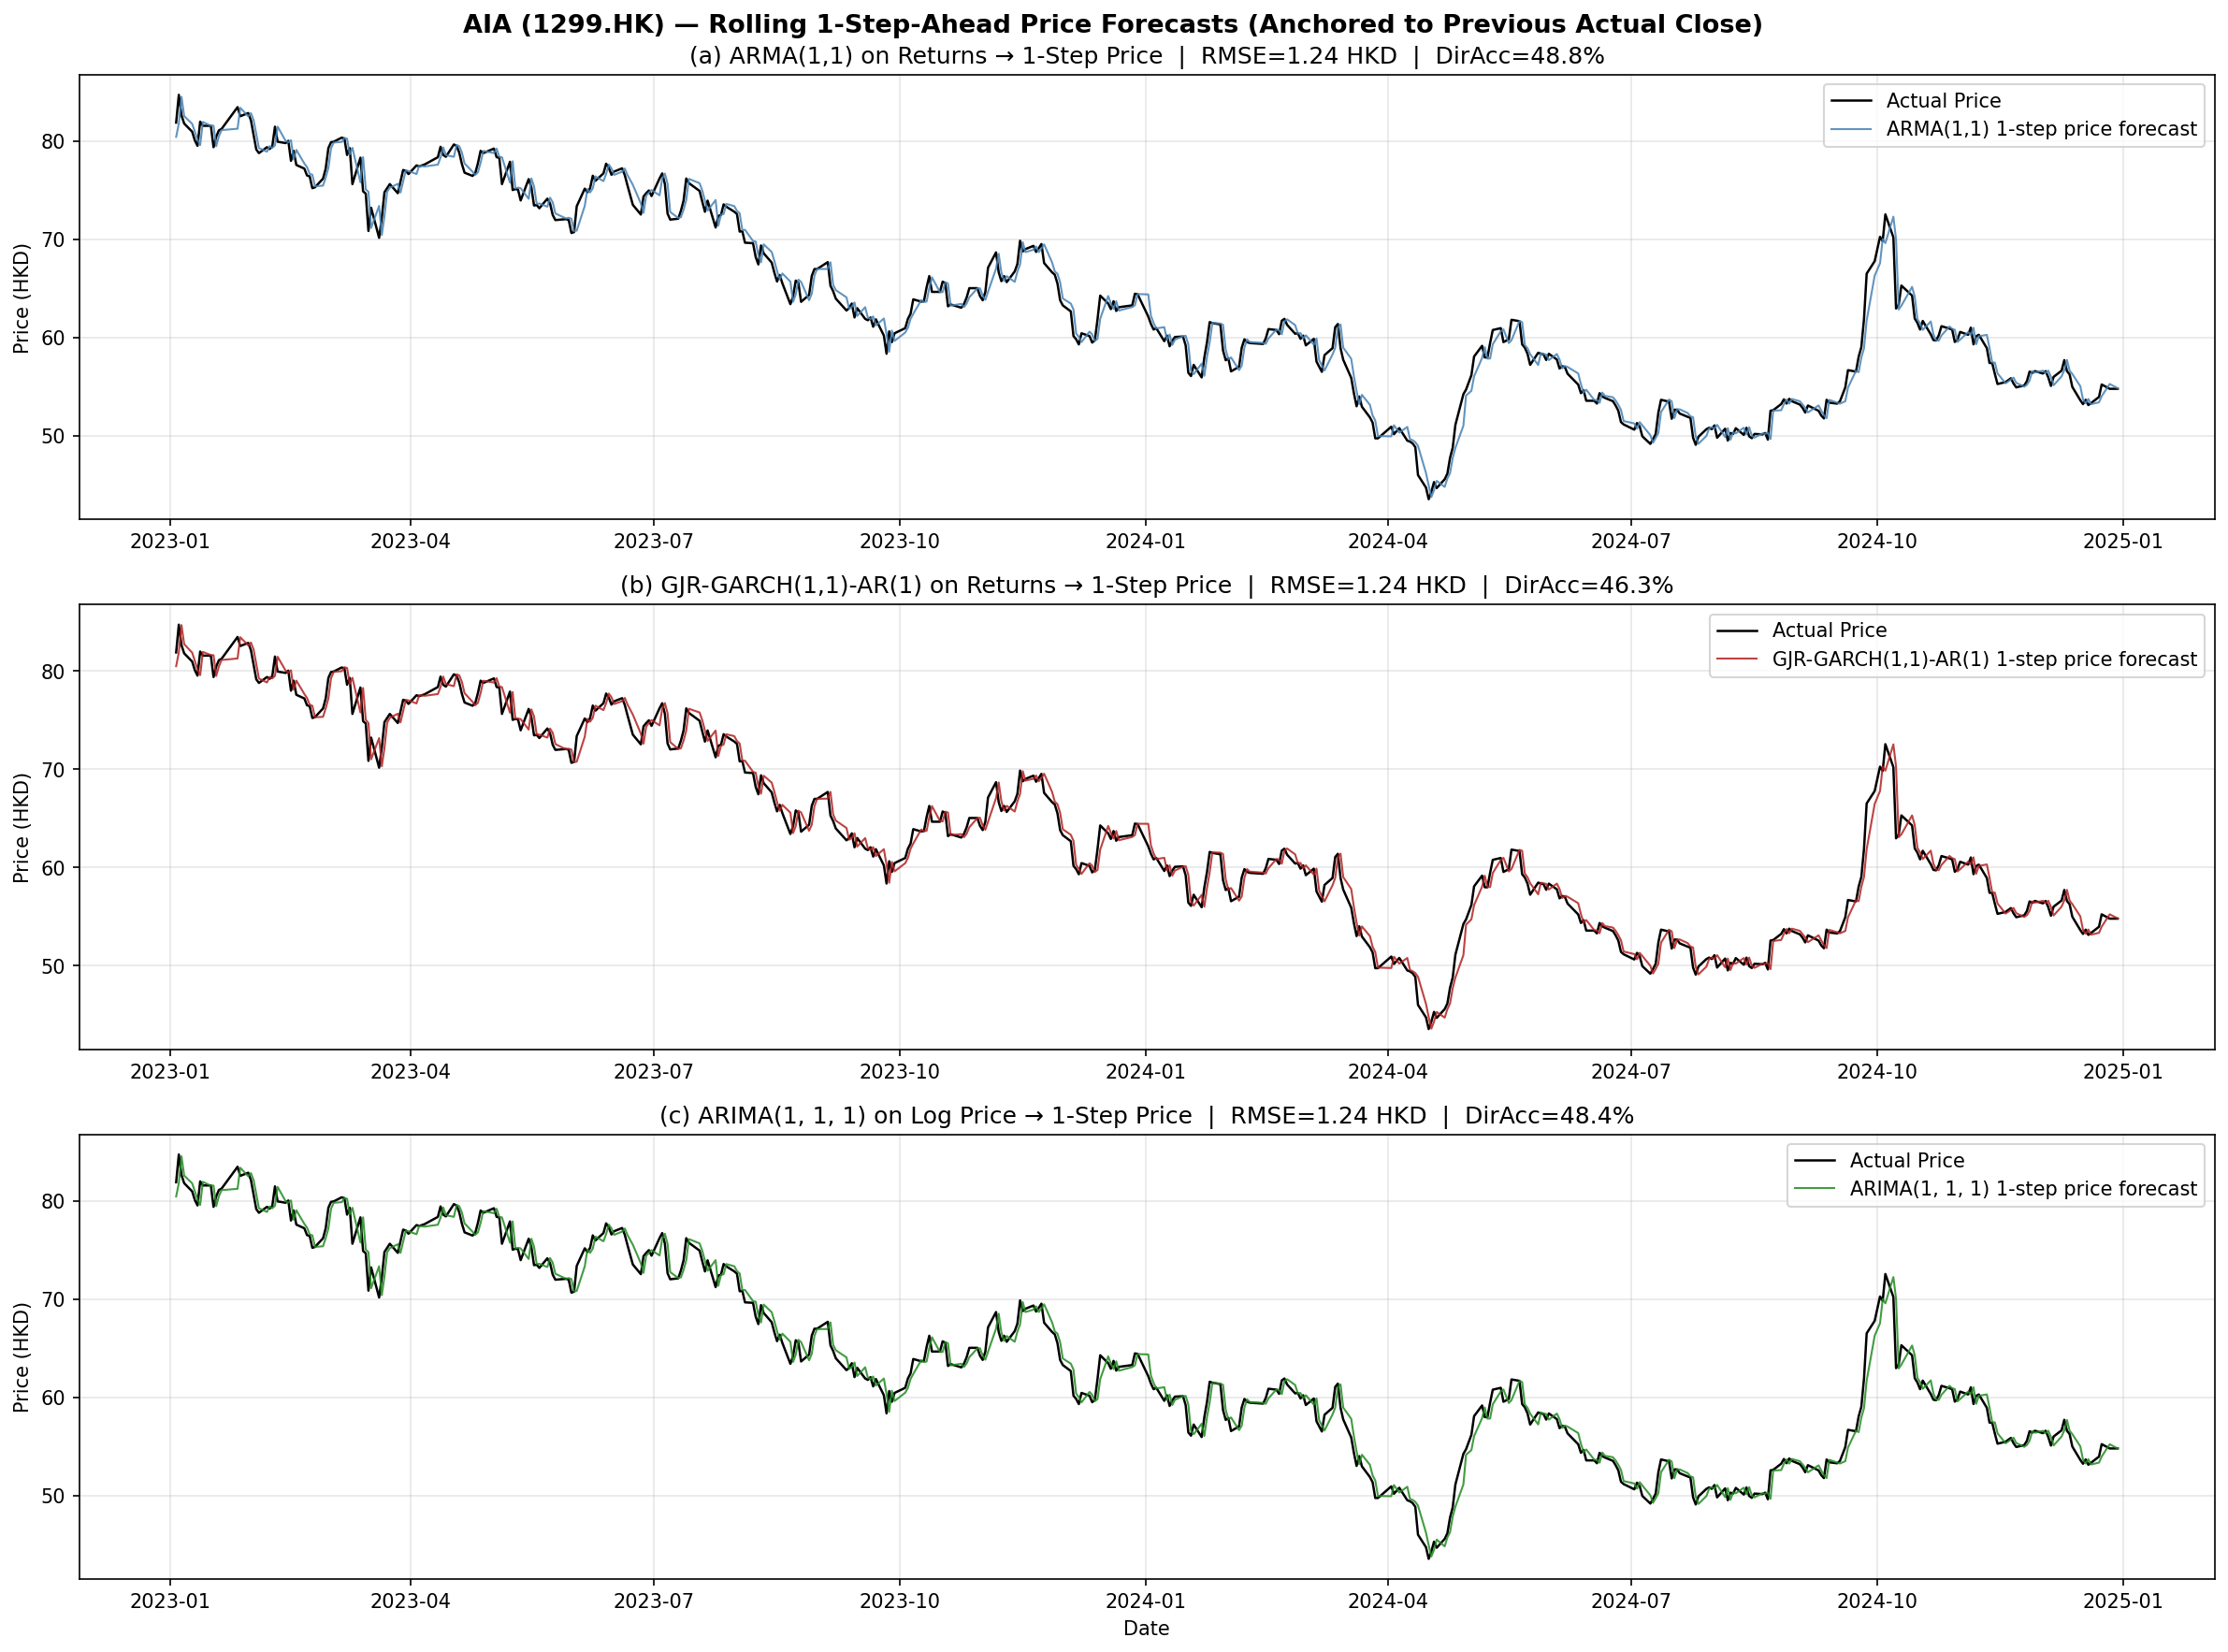
\includegraphics[width=0.95\linewidth]{aia_figure7_price_forecast.png}
\caption{AIA rolling one-step-ahead price forecast vs actual (2023--2024).
Top panel: ARMA(1,1).  Middle panel: GJR-GARCH(1,1)-AR(1).  Bottom panel:
ARIMA(1,1,1).  All models use price re-anchoring $P_{t+1} = P_t \times
\exp(\hat{r}_{t+1}/100)$; RMSEs are close to 1.24 HKD across all three
specifications.}
\label{fig:aia-fc}
\end{figure}

\begin{table}[H]
\centering
\small
\begin{tabular}{lrrr}
\toprule
model & RMSE (\%) & MAE (\%) & Directional Acc.\ (\%) \\
\midrule
ARMA(1,1)                & 1.9447 & 1.45 & 48.77 \\
GJR-GARCH(1,1)-AR(1)     & 1.9396 & 1.44 & 46.31 \\
\bottomrule
\end{tabular}
\caption{AIA out-of-sample forecasting performance (return scale, 2023--2024).}
\label{tab:aia-fc}
\end{table}

\subsection{Individual Conclusion -- AIA}
AIA daily log returns are stationary (ADF $p < 0.001$) and exhibit
statistically significant but economically weak serial correlation,
consistent with semi-strong market efficiency.  The optimal ARMA(1,1)
mean model captures short-term return dynamics with clean residual
diagnostics (LB(12) $p = 0.717$).  Strong ARCH effects are confirmed,
and the GJR-GARCH(1,1) model is preferred by AIC.  Volatility
persistence is high ($\alpha+\beta = 0.952$, half-life $\approx 29$
days), and the positive leverage parameter ($\gamma = 0.045$) confirms
that negative returns amplify future volatility more than positive
returns -- a pattern typical of financial-sector stocks.

Out-of-sample directional accuracy is below $50\%$, confirming that
AIA's predictability lives in its \emph{variance} rather than its
\emph{mean}.  As an insurance-sector blue chip, AIA provides a useful
intermediate-volatility benchmark between HSBC (banking) and Tencent
(technology), and its moderate correlation with the other three stocks
(Section~\ref{sec:compare-corr}) positions it as a ``bridge'' stock that
shares both financial-sector and broader market factors.

% =====================================================================
\section{Tencent Holdings (0700.HK)}
\label{sec:tencent}
\subsection{Data Description}

Tencent Holdings (0700.HK) represents the technology and internet sector. Its returns are expected to be relatively volatile because the stock is sensitive to growth expectations, regulation, and market sentiment.

The sample uses daily adjusted close prices from 2011-01-03 to 2024-12-31. The log return is defined as
\[
r_t = 100\left[\log(P_t)-\log(P_{t-1})\right],
\]
where \(P_t\) is the adjusted close price. The training period is 2011--2022, and the test period is 2023--2024.

Figure~\ref{fig:tencent-price-logprice} suggests that the price level is non-stationary, while Figure~\ref{fig:tencent-return} shows volatility clustering in daily returns.

\begin{figure}[H]
    \centering
    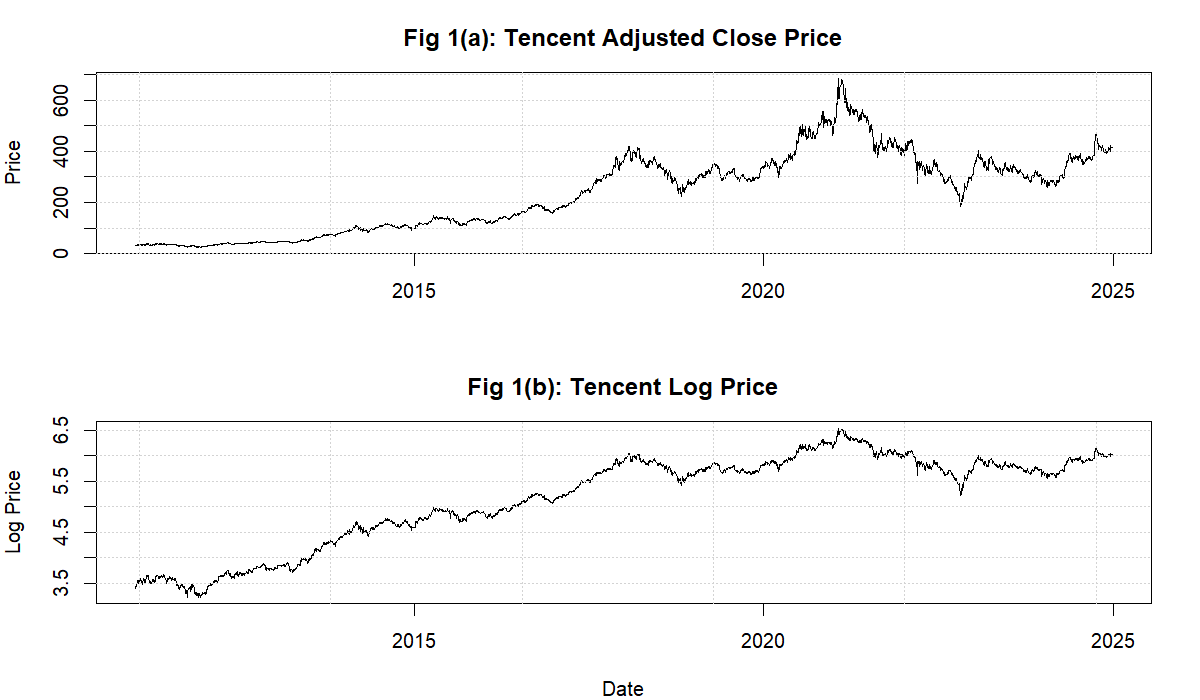
\includegraphics[width=0.72\textwidth]{C_figure/C_fig1_price_logprice.png}
    \caption{Tencent adjusted close price and log price}
    \label{fig:tencent-price-logprice}
\end{figure}

\begin{figure}[H]
    \centering
    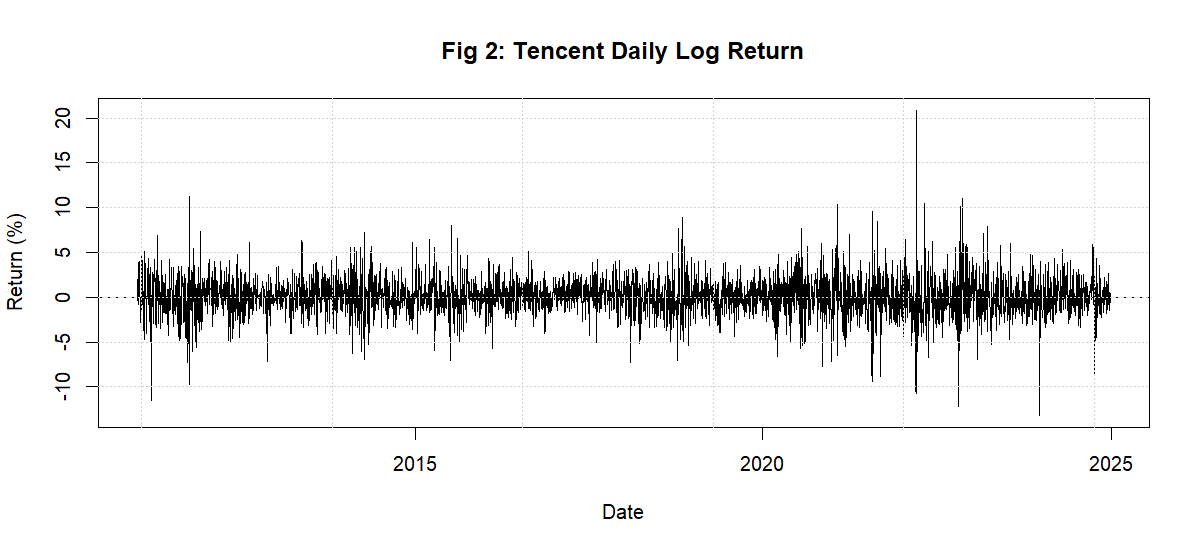
\includegraphics[width=0.72\textwidth]{C_figure/C_fig2_log_return.png}
    \caption{Tencent daily log return}
    \label{fig:tencent-return}
\end{figure}

\subsection{Preliminary Statistics}

Table~\ref{tab:tencent-descriptive} shows that Tencent's average daily return is small relative to its volatility. The return distribution is fat-tailed, with kurtosis far above 3, and the Jarque--Bera test rejects normality. This supports the use of models that allow non-normal and time-varying volatility.

\begin{table}[H]
\centering
\small
\caption{Descriptive statistics of Tencent daily log returns}
\label{tab:tencent-descriptive}
\resizebox{0.92\textwidth}{!}{
\begin{tabular}{lrrrrrrrr}
\toprule
Variable & Mean & Std. Dev. & Min & Max & Skewness & Kurtosis & Jarque--Bera & JB p-value \\
\midrule
Log return & 0.0760 & 2.1808 & -13.1796 & 20.8269 & 0.2004 & 8.1841 & 3983.96 & $<0.001$ \\
\bottomrule
\end{tabular}
}
\end{table}

\subsection{Stationarity and Serial Correlation}

Table~\ref{tab:tencent-tests} shows that the log price is non-stationary, while the log return is stationary. The Ljung--Box test on returns indicates some serial dependence, and the tests on squared returns strongly support conditional heteroskedasticity.

\begin{table}[H]
\centering
\small
\caption{Stationarity, serial correlation, and ARCH-effect tests for Tencent}
\label{tab:tencent-tests}
\begin{tabular}{lrr}
\toprule
Test & Statistic & p-value \\
\midrule
ADF on log price & -1.3017 & 0.8740 \\
ADF on log return & -14.3363 & $\leq 0.0100$ \\
Ljung--Box on returns, lag 20 & 40.5152 & 0.0043 \\
Ljung--Box on squared returns, lag 20 & 392.9963 & $<0.001$ \\
ARCH-LM on returns, lag 20 & 236.6664 & $5.51\times 10^{-39}$ \\
\bottomrule
\end{tabular}
\end{table}

Figures~\ref{fig:tencent-acf-pacf} and~\ref{fig:tencent-squared-acf} are consistent with these results. The return ACF/PACF motivates low-order ARMA models, while the squared-return ACF supports the use of GARCH-type volatility models.

\begin{figure}[H]
    \centering
    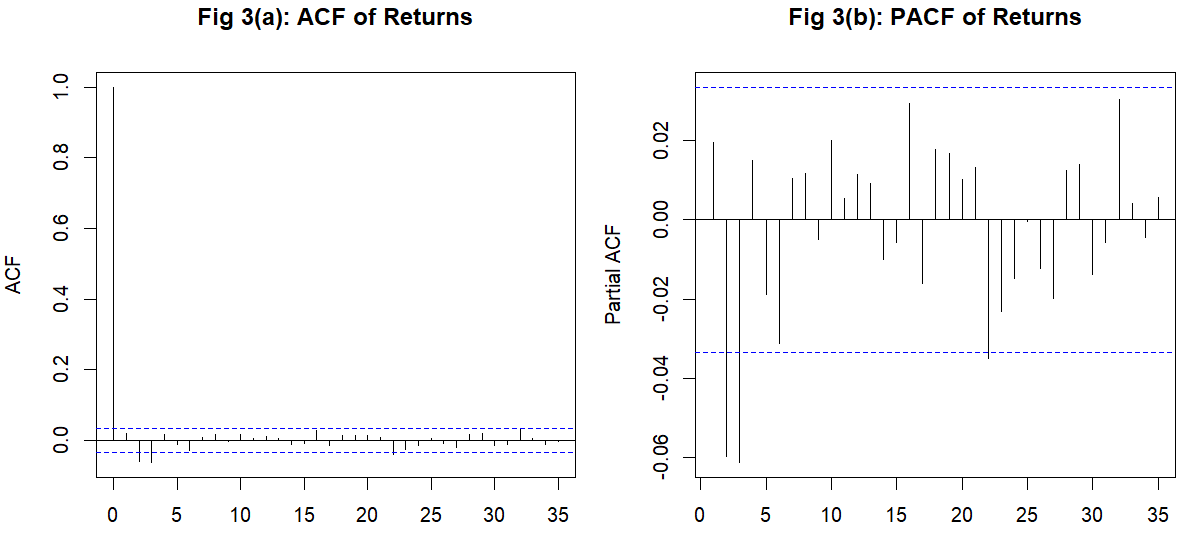
\includegraphics[width=0.66\textwidth]{C_figure/C_fig3_acf_pacf_returns.png}
    \caption{ACF and PACF of Tencent returns}
    \label{fig:tencent-acf-pacf}
\end{figure}

\begin{figure}[H]
    \centering
    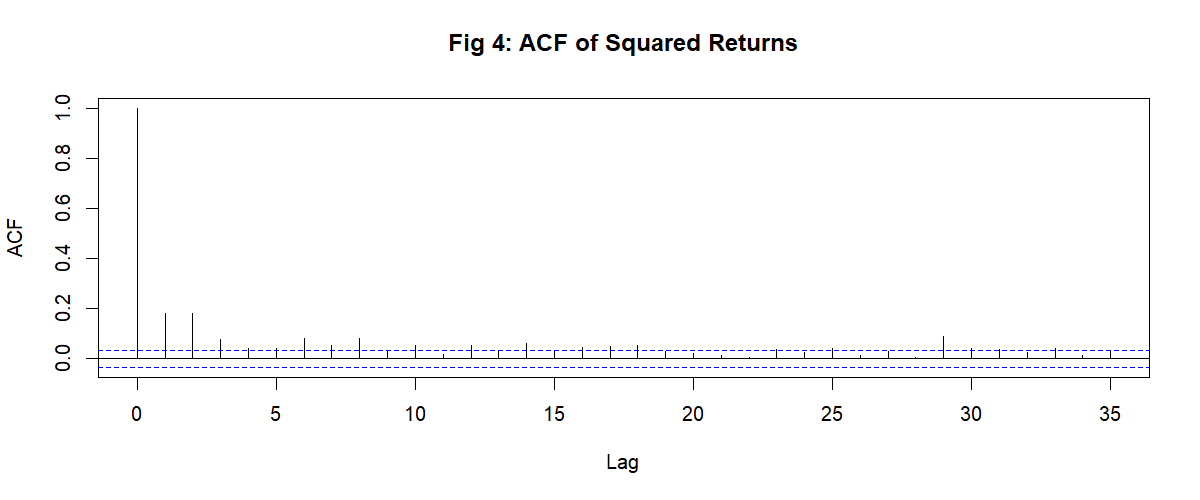
\includegraphics[width=0.66\textwidth]{C_figure/C_fig4_squared_return_acf.png}
    \caption{ACF of squared Tencent returns}
    \label{fig:tencent-squared-acf}
\end{figure}

\subsection{ARMA Mean Model}

Based on Figure~\ref{fig:tencent-acf-pacf}, seven low-order ARMA models are compared, covering pure AR, pure MA, and mixed ARMA specifications. AIC and BIC are used for model selection, while the Ljung--Box test checks residual serial correlation.

\begin{table}[H]
\centering
\small
\caption{ARMA models for Tencent returns}
\label{tab:tencent-arma-candidates}
\resizebox{0.98\textwidth}{!}{
\begin{tabular}{lrrrrrr}
\toprule
Model & $p$ & $q$ & AIC & BIC & Residual LB(20) p-value & Residual ARCH-LM(10) p-value \\
\midrule
ARMA(0,3) & 0 & 3 & 13030.82 & 13060.77 & 0.8806 & $6.19\times 10^{-39}$ \\
ARMA(2,1) & 2 & 1 & 13037.17 & 13067.13 & 0.5602 & $3.65\times 10^{-40}$ \\
ARMA(2,2) & 2 & 2 & 13038.35 & 13074.30 & 0.5999 & $1.99\times 10^{-39}$ \\
ARMA(0,2) & 0 & 2 & 13045.60 & 13069.57 & 0.1104 & $2.90\times 10^{-41}$ \\
ARMA(0,1) & 0 & 1 & 13055.34 & 13073.32 & 0.0047 & $1.83\times 10^{-41}$ \\
ARMA(1,1) & 1 & 1 & 13055.52 & 13079.48 & 0.0092 & $1.85\times 10^{-40}$ \\
ARMA(1,0) & 1 & 0 & 13055.58 & 13073.55 & 0.0042 & $7.21\times 10^{-42}$ \\
\bottomrule
\end{tabular}
}
\end{table}

Table~\ref{tab:tencent-arma-candidates} shows that ARMA(0,3) has the lowest AIC and BIC. Its residual Ljung--Box p-value is 0.8806, indicating no significant remaining linear serial correlation. Therefore, ARMA(0,3) is selected as the mean model.

However, the ARCH-LM p-value remains highly significant at \(6.19\times 10^{-39}\). Thus, ARMA(0,3) controls the conditional mean but not the conditional variance, motivating GARCH-family models. Figure~\ref{fig:tencent-arma-residuals} reports the corresponding residual diagnostics.

\begin{figure}[H]
    \centering
    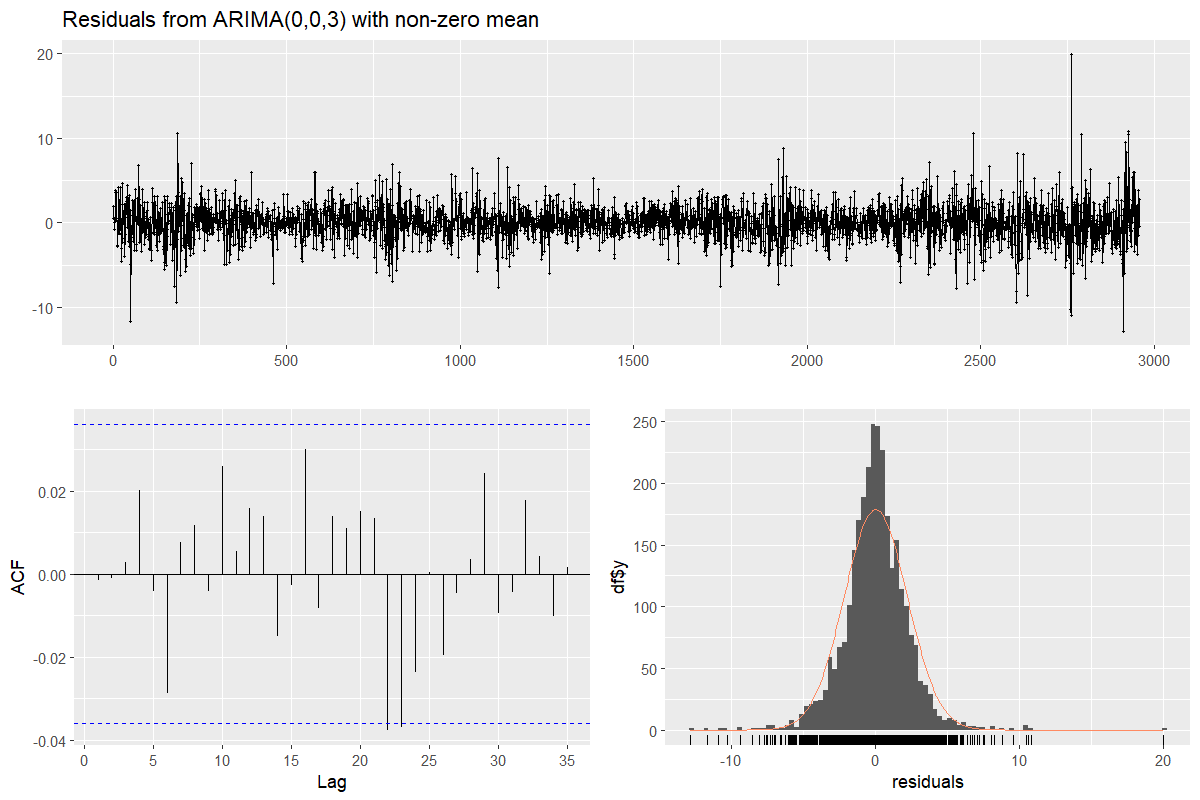
\includegraphics[width=0.64\textwidth]{C_figure/C_fig5_check_arma_residuals.png}
    \caption{Residual diagnostics for the selected ARMA(0,3) model}
    \label{fig:tencent-arma-residuals}
\end{figure}

\subsection{Volatility Model}

The significant ARCH effect indicates time-varying volatility. Therefore, GARCH(1,1), EGARCH(1,1), and GJR-GARCH(1,1) are compared, both with a constant mean and with the selected ARMA(0,3) mean equation.

\begin{table}[H]
\centering
\small
\caption{Comparison of GARCH-family models for Tencent returns}
\label{tab:tencent-garch-comparison}
\resizebox{0.98\textwidth}{!}{
\begin{tabular}{llrrrr}
\toprule
Model group & Model & AIC & BIC & $\alpha_1+\beta_1$ & Asymmetry / leverage \\
\midrule
Constant mean & GARCH(1,1) & 4.2181 & 4.2272 & 0.9700 & -- \\
Constant mean & EGARCH(1,1) & 4.2148 & 4.2270 & 0.9039 & 0.1655 \\
Constant mean & GJR-GARCH(1,1) & 4.2148 & 4.2269 & 0.9229 & 0.0910 \\
ARMA(0,3) mean & ARMA-GARCH(1,1) & 4.2151 & 4.2333 & 0.9700 & -- \\
ARMA(0,3) mean & ARMA-EGARCH(1,1) & 4.2118 & 4.2300 & 0.9103 & 0.1624 \\
ARMA(0,3) mean & ARMA-GJR-GARCH(1,1) & 4.2118 & 4.2300 & 0.9253 & 0.0853 \\
\bottomrule
\end{tabular}
}
\end{table}

Table~\ref{tab:tencent-garch-comparison} shows that GJR-GARCH(1,1) is preferred among the constant-mean models. Its positive leverage parameter indicates that negative shocks increase future volatility more strongly than positive shocks.

After adding the ARMA(0,3) mean equation, ARMA-GJR-GARCH(1,1) is selected as the final volatility model. It has the lowest AIC among the ARMA-GARCH specifications and retains a positive leverage effect, indicating persistent and asymmetric volatility.

Figures~\ref{fig:tencent-garch-volatility}--\ref{fig:tencent-arma-garch-residual-acf} show the fitted volatility and residual diagnostics. The final standardized residual tests are satisfactory, with Ljung--Box p-values of 0.5990 and 0.8658 for standardized and squared standardized residuals, and ARCH-LM p-value of 0.8708.

\begin{figure}[H]
    \centering
    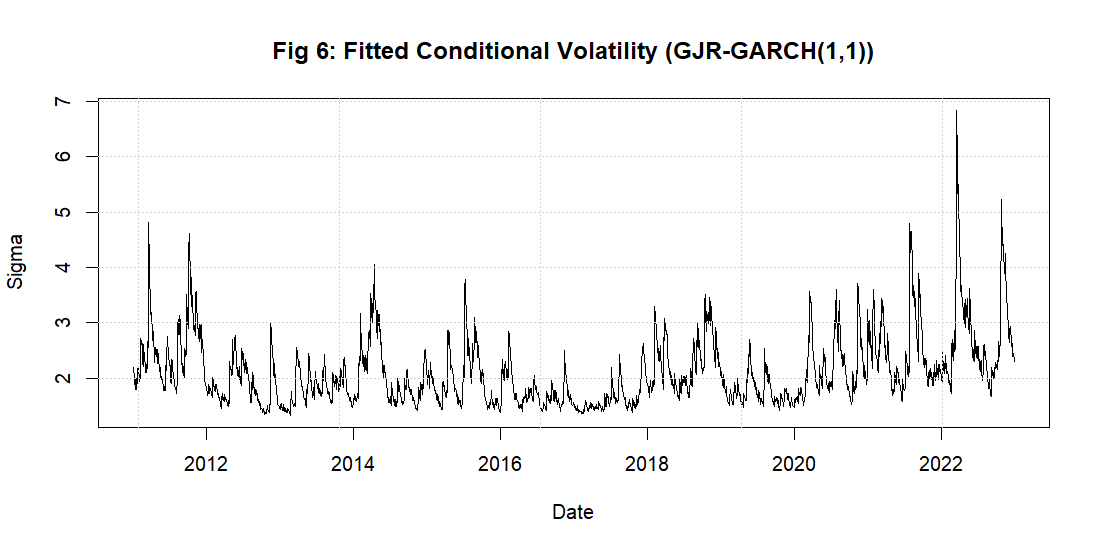
\includegraphics[width=0.64\textwidth]{C_figure/C_fig6_garch_fitted_conditional_volatility.png}
    \caption{Fitted conditional volatility from the selected GARCH model}
    \label{fig:tencent-garch-volatility}
\end{figure}

\begin{figure}[H]
    \centering
    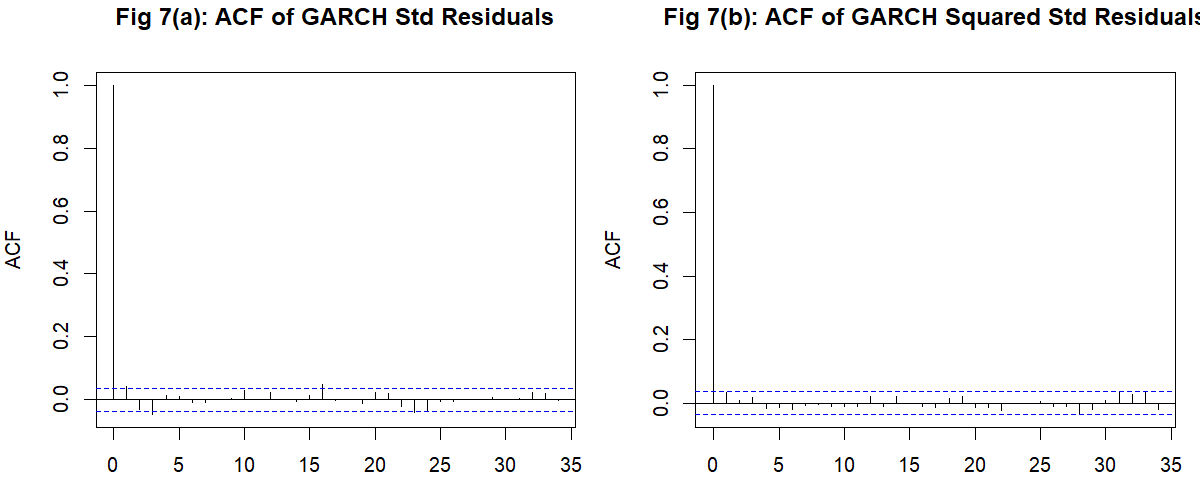
\includegraphics[width=0.64\textwidth]{C_figure/C_fig7_garch_standardized_residuals_acf.png}
    \caption{ACF of standardized residuals and squared standardized residuals from the selected GARCH model}
    \label{fig:tencent-garch-residual-acf}
\end{figure}

\begin{figure}[H]
    \centering
    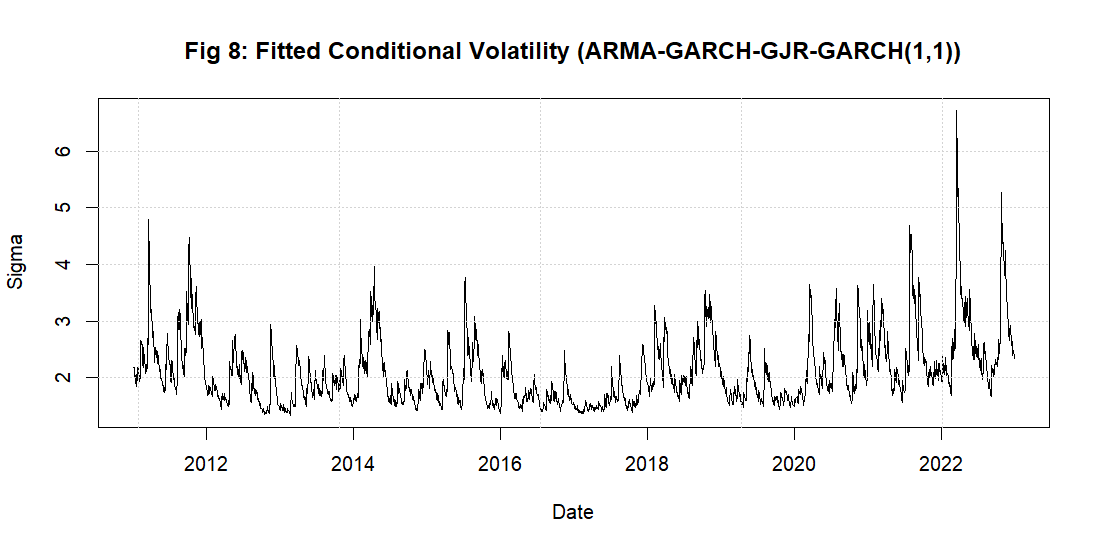
\includegraphics[width=0.64\textwidth]{C_figure/C_fig8_arma_garch_fitted_conditional_volatility.png}
    \caption{Fitted conditional volatility from the ARMA-GJR-GARCH(1,1) model}
    \label{fig:tencent-arma-garch-volatility}
\end{figure}

\begin{figure}[H]
    \centering
    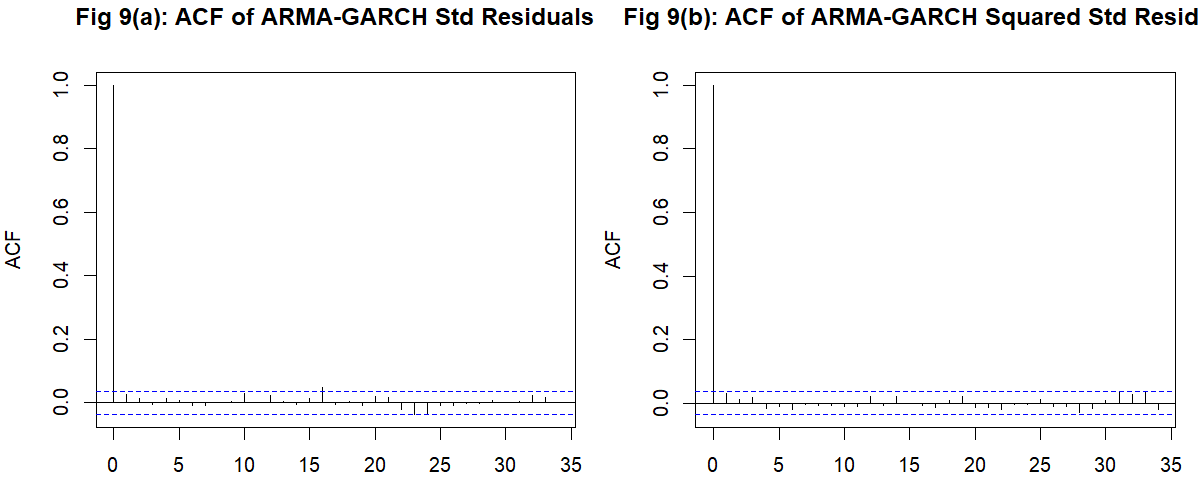
\includegraphics[width=0.64\textwidth]{C_figure/C_fig9_arma_garch_standardized_residuals_acf.png}
    \caption{ACF of standardized residuals and squared standardized residuals from the selected ARMA-GJR-GARCH(1,1) model}
    \label{fig:tencent-arma-garch-residual-acf}
\end{figure}

\subsection{Forecasting}

Forecasting is evaluated over 2023--2024 using RMSE, MAE, and directional accuracy. Table~\ref{tab:tencent-forecast} shows that GJR-GARCH(1,1) has the lowest RMSE and MAE, while ARMA-GJR-GARCH(1,1) has the highest directional accuracy.

\begin{table}[H]
\centering
\small
\caption{Forecasting performance for Tencent during 2023--2024}
\label{tab:tencent-forecast}
\resizebox{0.92\textwidth}{!}{
\begin{tabular}{llrrr}
\toprule
Model & Specification & RMSE & MAE & Directional accuracy (\%) \\
\midrule
Rolling ARMA & ARMA(0,3) & 2.0740 & 1.5479 & 48.36 \\
Rolling GARCH & GJR-GARCH(1,1) & 2.0662 & 1.5373 & 47.54 \\
Rolling ARMA-GARCH & ARMA-GJR-GARCH(1,1) & 2.0695 & 1.5433 & 50.00 \\
\bottomrule
\end{tabular}
}
\end{table}

Figures~\ref{fig:tencent-return-forecast} and~\ref{fig:tencent-vol-forecast} show that return forecasts remain close to zero, while volatility forecasts better track changes in risk. This suggests that GARCH-type models are more useful for volatility forecasting than for daily return point forecasting.

\begin{figure}[H]
    \centering
    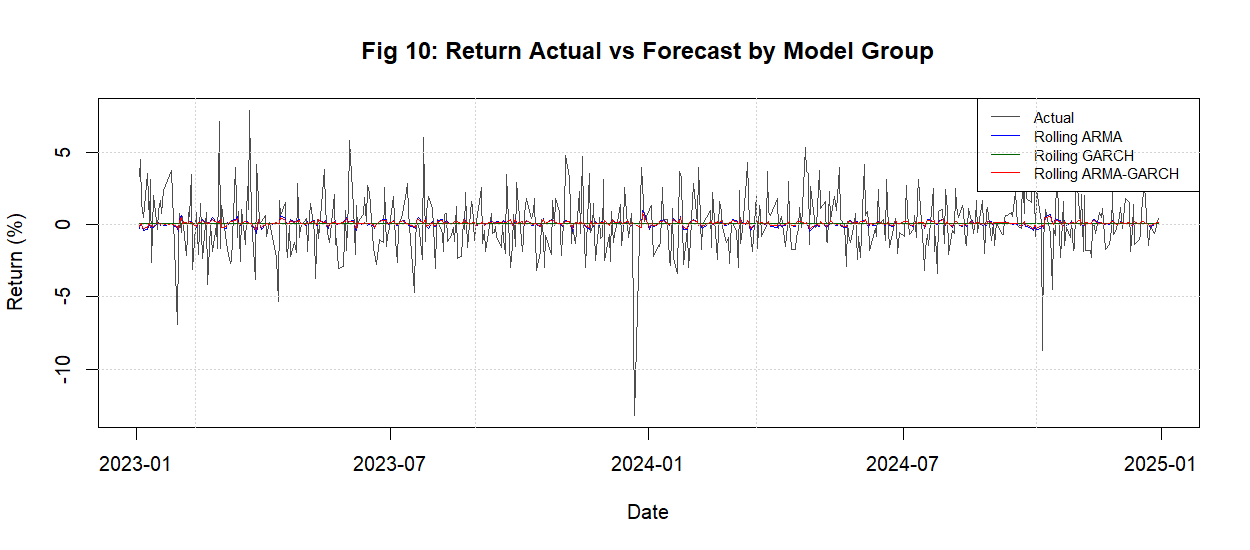
\includegraphics[width=0.72\textwidth]{C_figure/C_fig10_return_forecast_three_groups.png}
    \caption{Actual Tencent returns versus return forecasts}
    \label{fig:tencent-return-forecast}
\end{figure}

\begin{figure}[H]
    \centering
    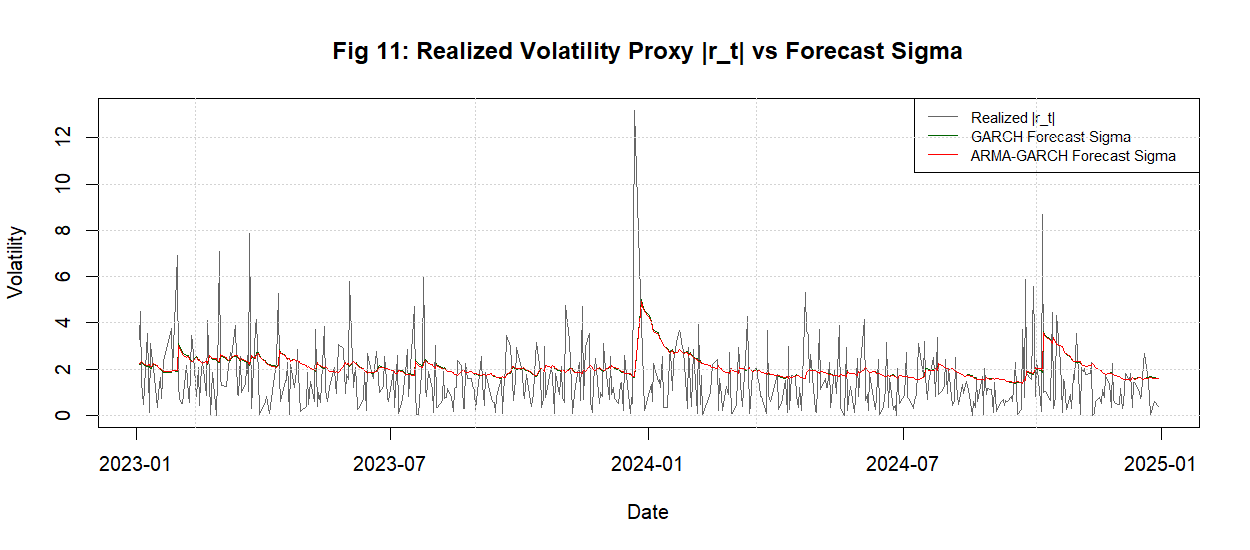
\includegraphics[width=0.72\textwidth]{C_figure/C_fig11_volatility_forecast_three_groups.png}
    \caption{Realized volatility proxy and forecast volatility for Tencent}
    \label{fig:tencent-vol-forecast}
\end{figure}

For the price-level forecast, GJR-GARCH(1,1) gives a price RMSE of 7.1284, a price MAE of 5.2472, and a directional accuracy of 47.54\%. Figure~\ref{fig:tencent-price-forecast} shows that the predicted price follows the broad level of the actual price but misses short-term movements.

\begin{figure}[H]
    \centering
    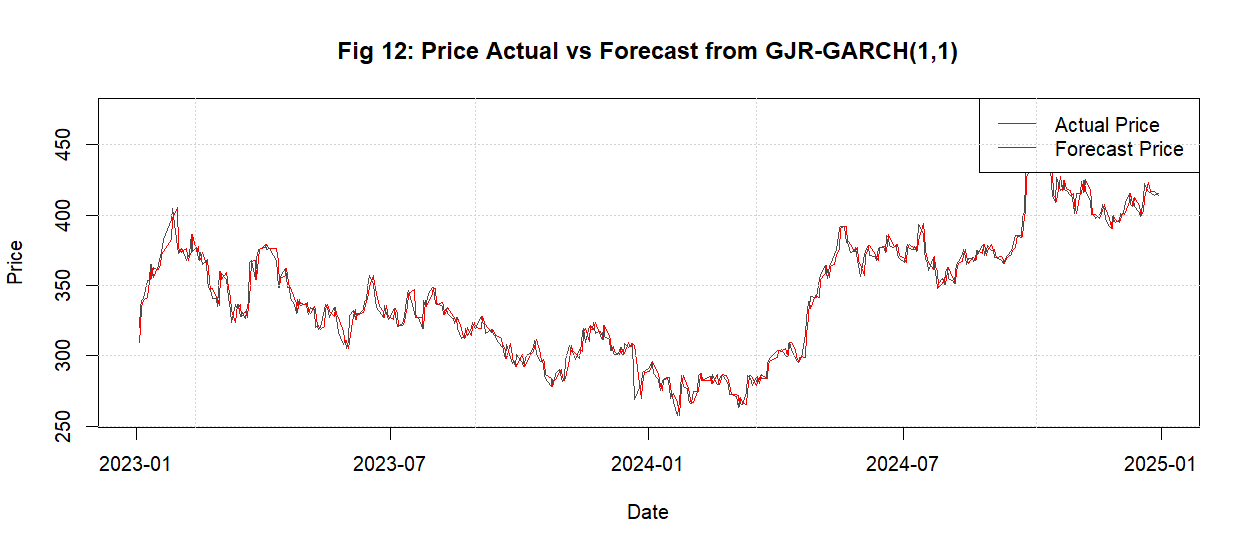
\includegraphics[width=0.72\textwidth]{C_figure/C_fig12_price_forecast_supplementary.png}
    \caption{Tencent price forecast}
    \label{fig:tencent-price-forecast}
\end{figure}

\subsection{Individual Conclusion}

Tencent's log return is stationary but fat-tailed and volatile. ARMA(0,3) removes most linear serial correlation, but strong ARCH effects remain, so a separate volatility model is required.

The selected ARMA-GJR-GARCH(1,1) model shows persistent and asymmetric volatility. Negative shocks have stronger effects on future volatility, consistent with Tencent's sensitivity to market sentiment, regulation, and growth expectations.

Forecasting results show limited daily return predictability, but stronger volatility predictability. Therefore, Tencent is better characterized by predictable risk rather than predictable daily returns.
% =====================================================================
\section{CLP Holdings (0002.HK)}
\label{sec:clp}

\subsection{Data Description}
CLP is a large HK utility and is used here as the defensive benchmark.
The sample period is 2011-01-03 to 2024-12-31, giving $3{,}446$ usable
log-return observations.  The price series shows a long-run upward
trend, while the return series fluctuates around zero with visible
volatility clustering -- the standard non-stationary-price /
stationary-return contrast.

\begin{figure}[H]
\centering
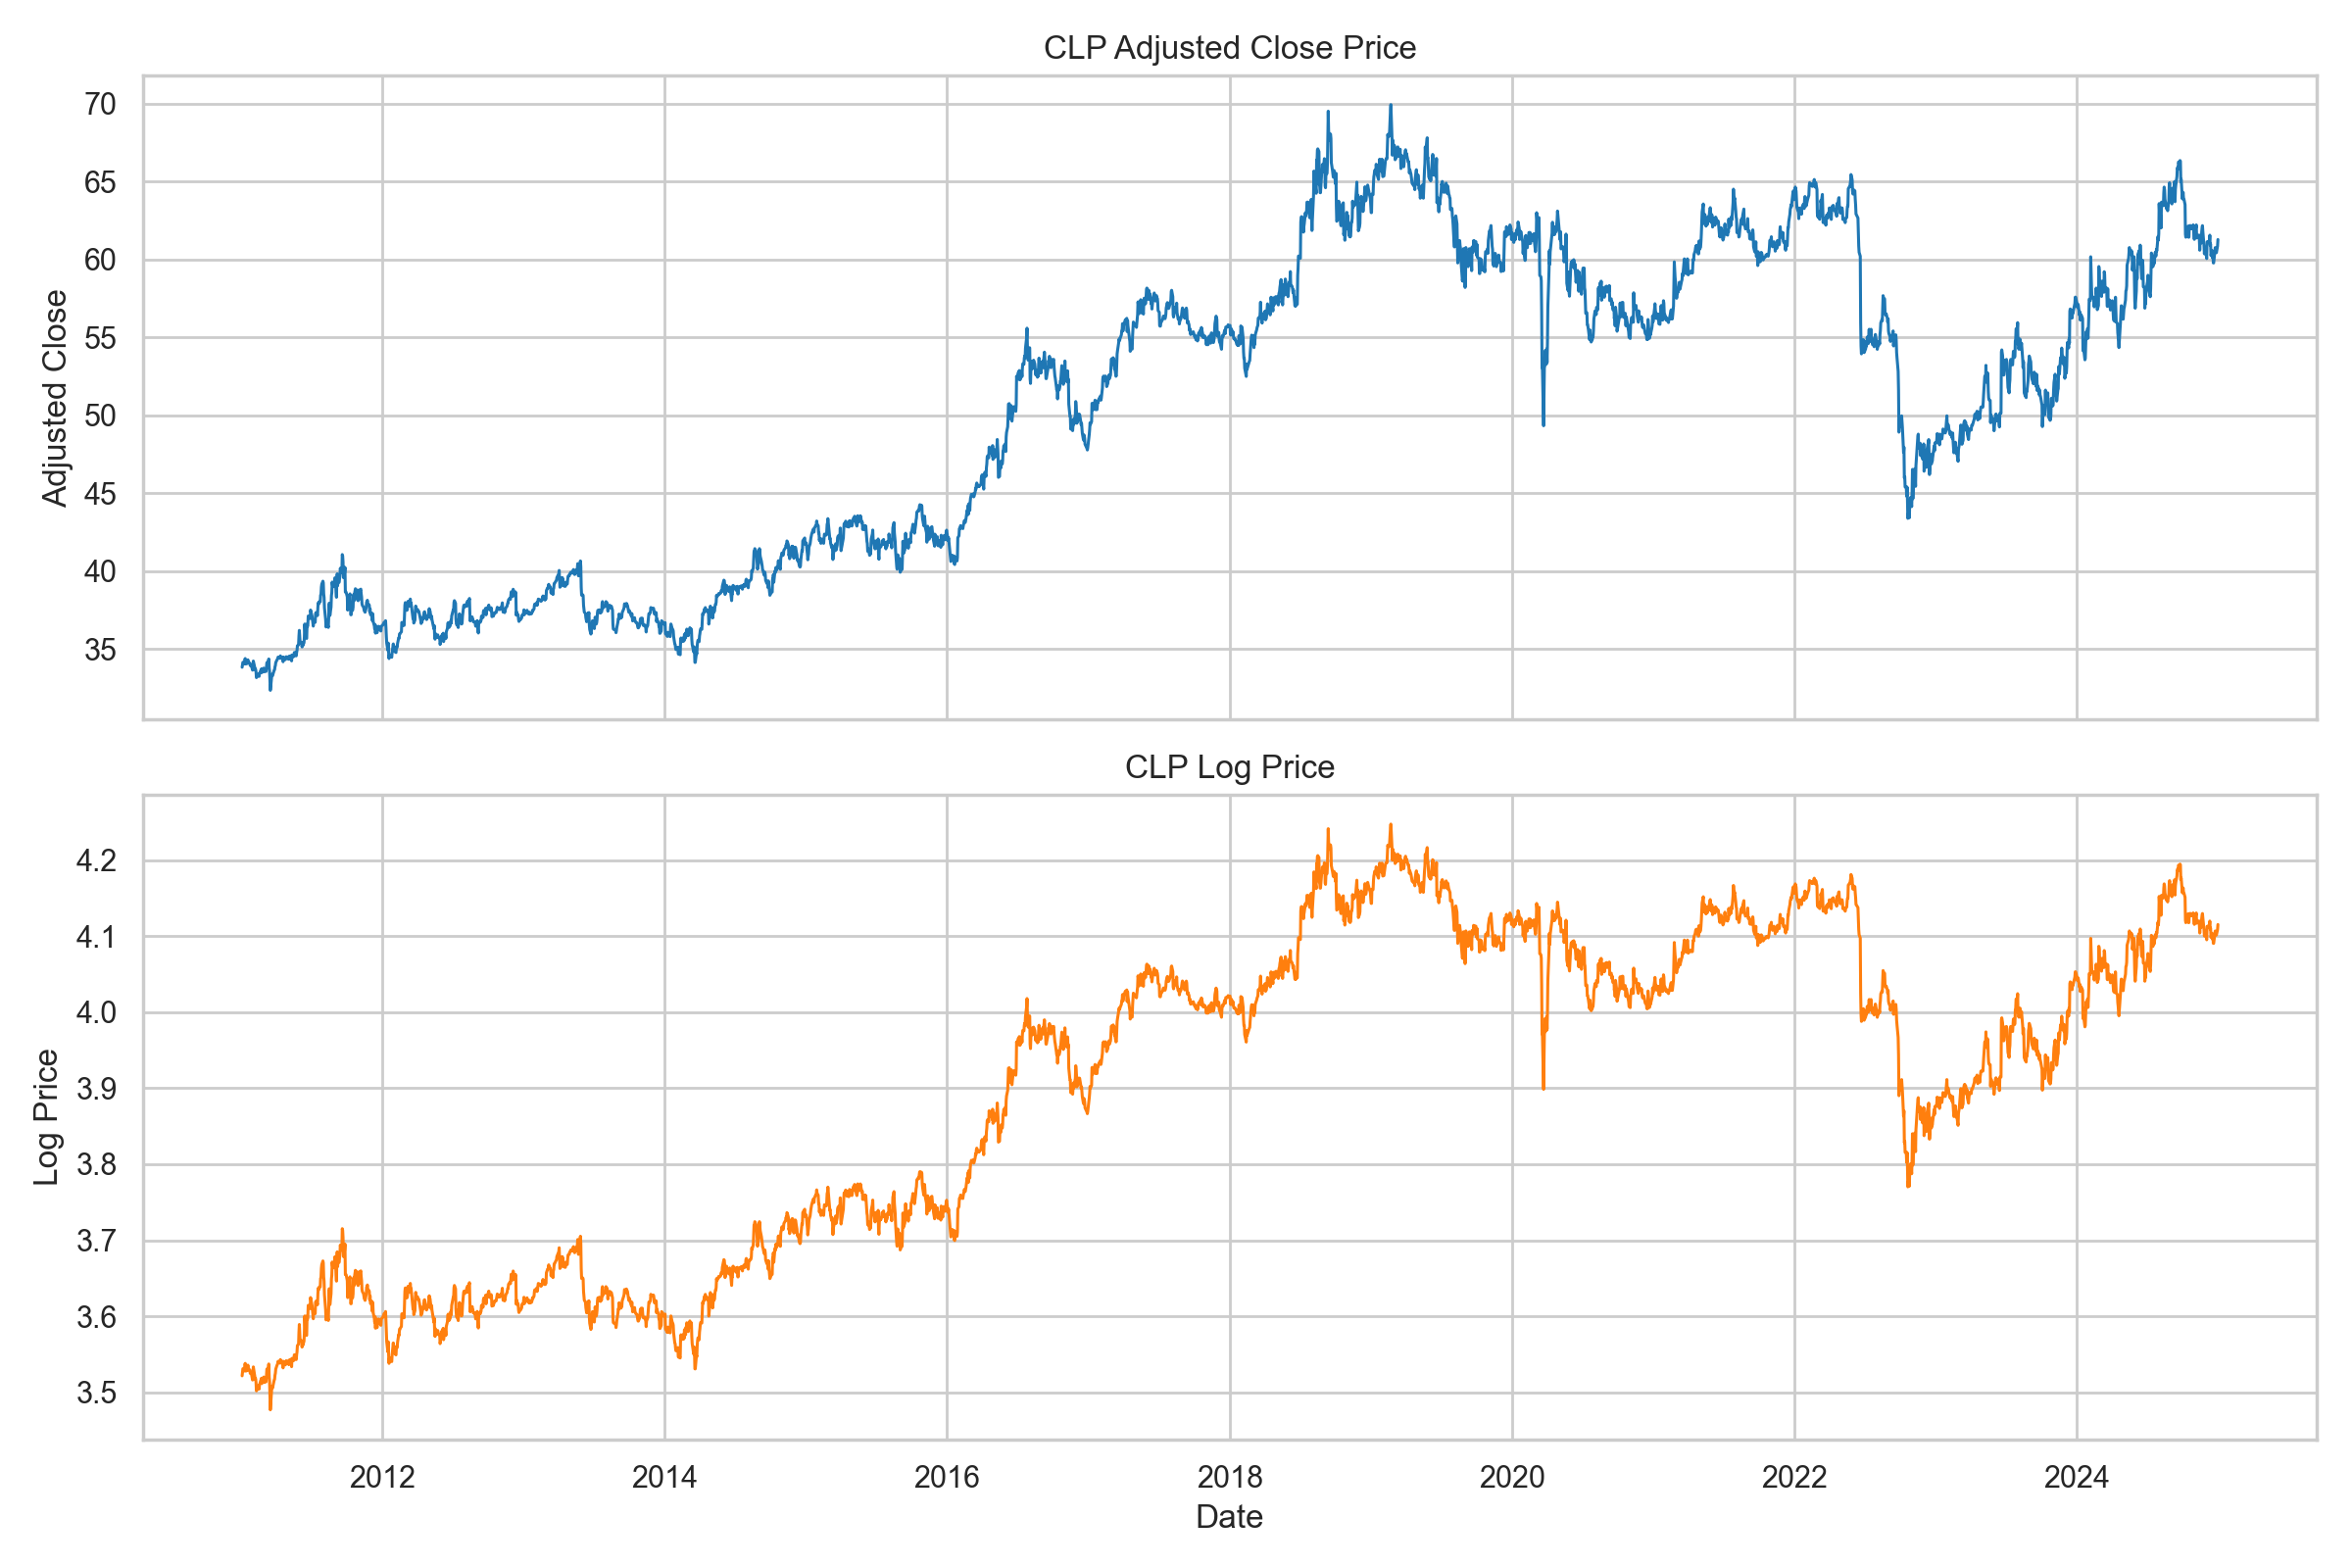
\includegraphics[width=0.95\linewidth]{figure1_price_and_log_price.png}
\caption{CLP price and log price (2011--2024).}
\label{fig:clp-price}
\end{figure}

\begin{figure}[H]
\centering
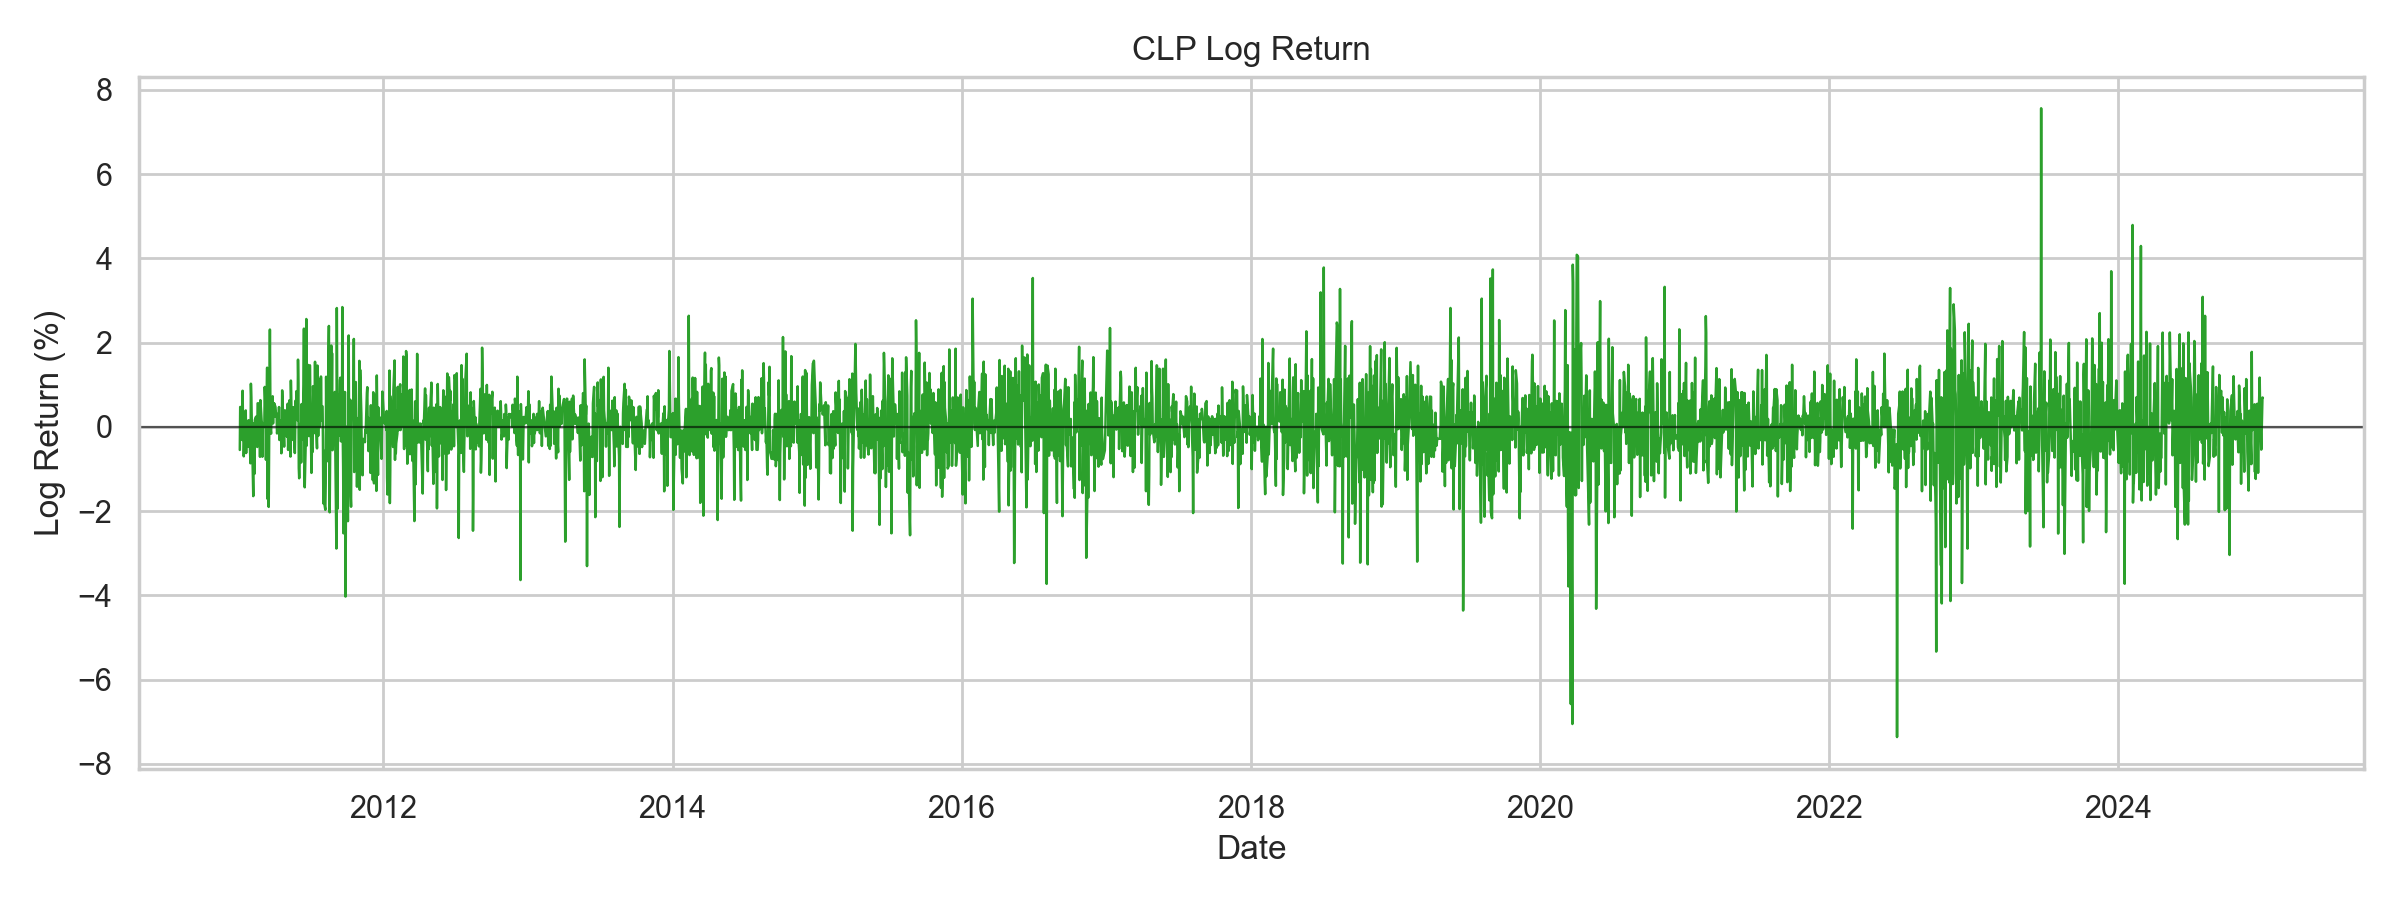
\includegraphics[width=0.95\linewidth]{figure2_log_return_plot.png}
\caption{CLP daily log return (\%) (2011--2024).}
\label{fig:clp-return}
\end{figure}

\subsection{Preliminary Statistics}
Mean daily log return is $0.0171\%$ and standard deviation is
$0.9643\%$.  Min/max daily returns are $-7.36\%$ and $+7.56\%$.
Skewness is $-0.298$ (mild left tail) and kurtosis is $5.44$, well
above 3.  The Jarque--Bera statistic is $4279.80$ with $p \approx 0$,
so normality is firmly rejected.  Hence a Gaussian homoskedastic
assumption is inappropriate and a volatility model is needed.  Among
the four stocks in this project, CLP also has the lowest unconditional
volatility, which is consistent with its role as the defensive
benchmark in the cross-stock comparison.

\begin{table}[H]
\centering
\small
\csvtab{../output/clp/tables/table1_descriptive_statistics.csv}
\caption{CLP descriptive statistics (daily log return, \%).}
\label{tab:clp-desc}
\end{table}

\subsection{Stationarity and Serial Correlation}
ADF on log price gives $-1.62$ ($p = 0.47$): a unit root cannot be
rejected.  ADF on log return gives $-18.35$ ($p \approx 2.2\!\times\!10^{-30}$):
returns are strongly stationary.

Ljung--Box on raw returns is only borderline at lag~10 ($p=0.0505$)
and lag~20 ($p=0.0933$): mean dependence is weak.  However,
Ljung--Box on \emph{squared} returns is highly significant at every
horizon -- volatility clustering is unambiguous.  This is the standard
signal that the mean equation can stay simple, while the conditional
variance should be modeled explicitly.

\begin{figure}[H]
\centering
\begin{subfigure}{0.49\linewidth}
  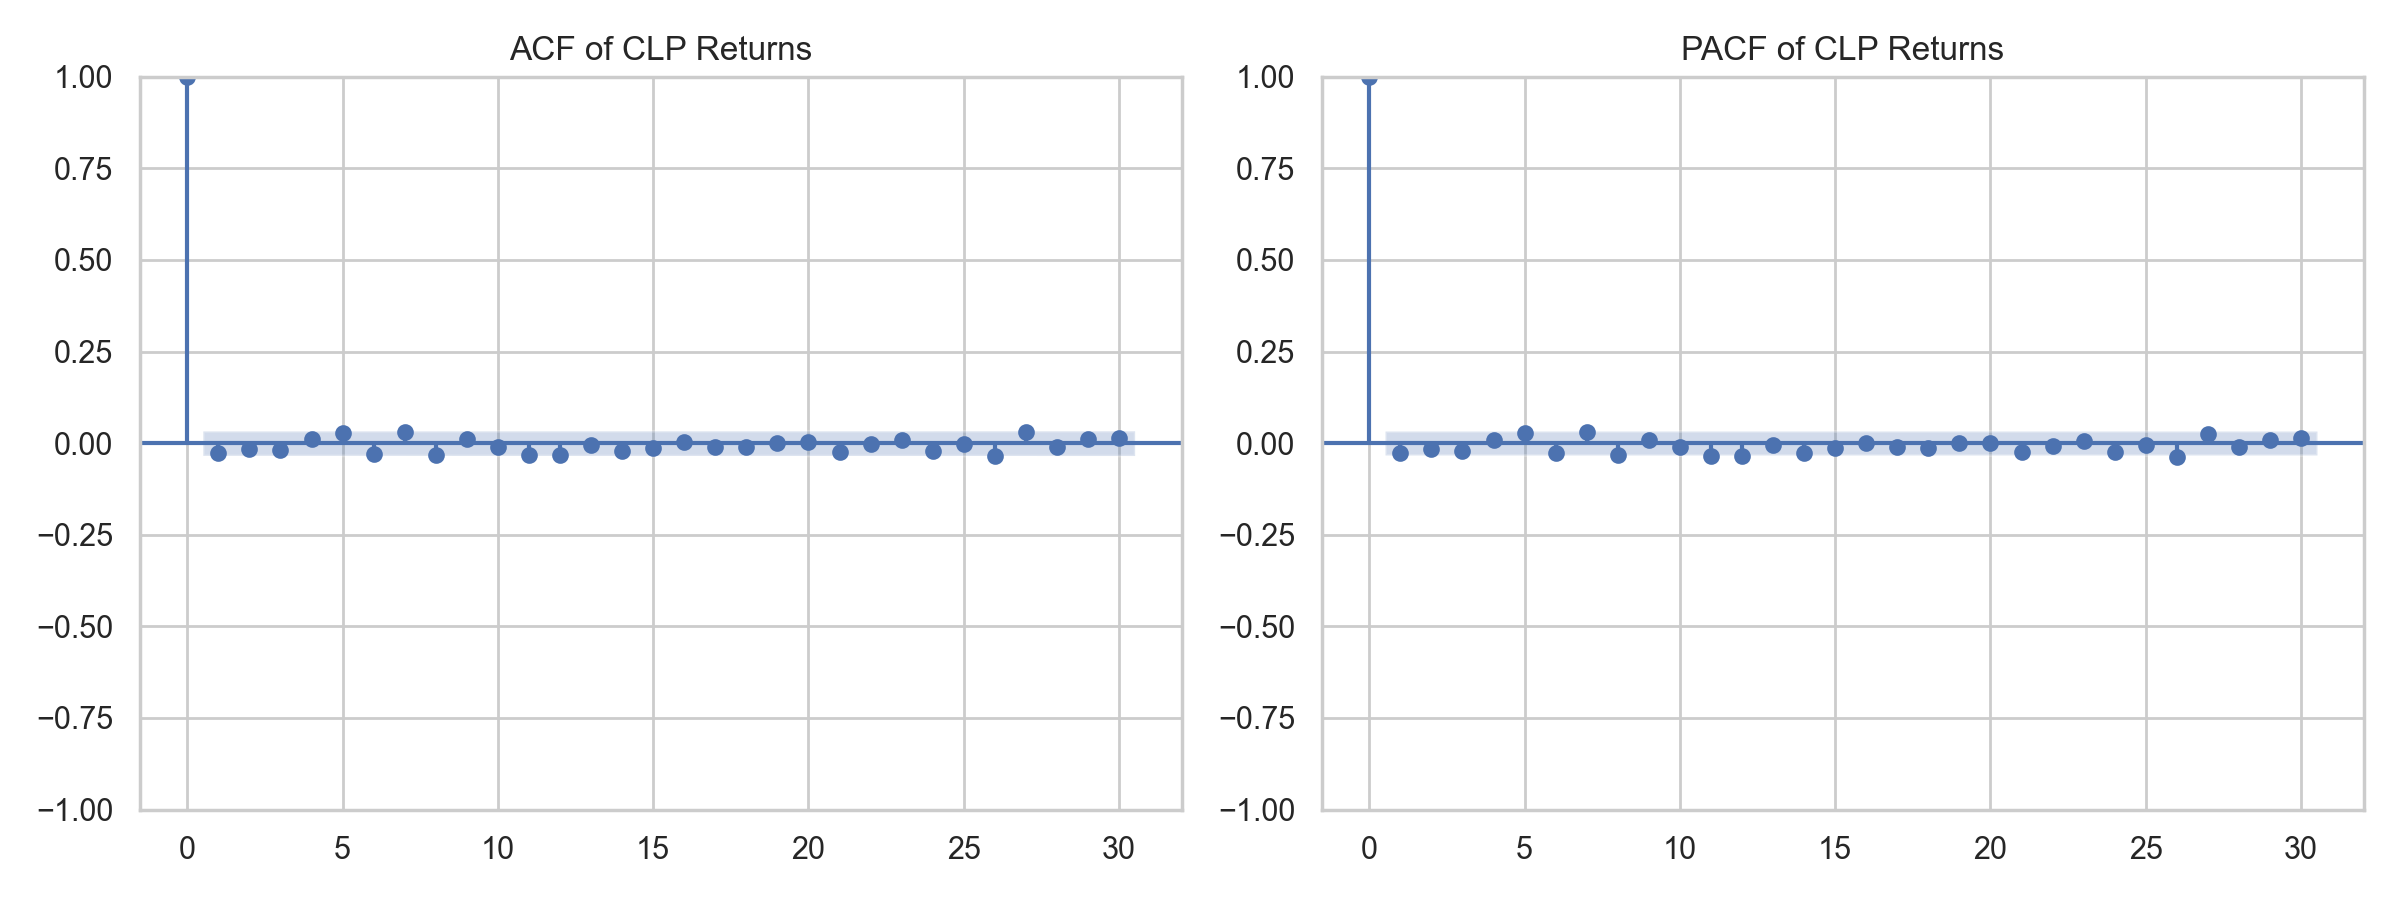
\includegraphics[width=\linewidth]{figure3_acf_pacf_returns.png}
  \caption{ACF/PACF of returns}
\end{subfigure}\hfill
\begin{subfigure}{0.49\linewidth}
  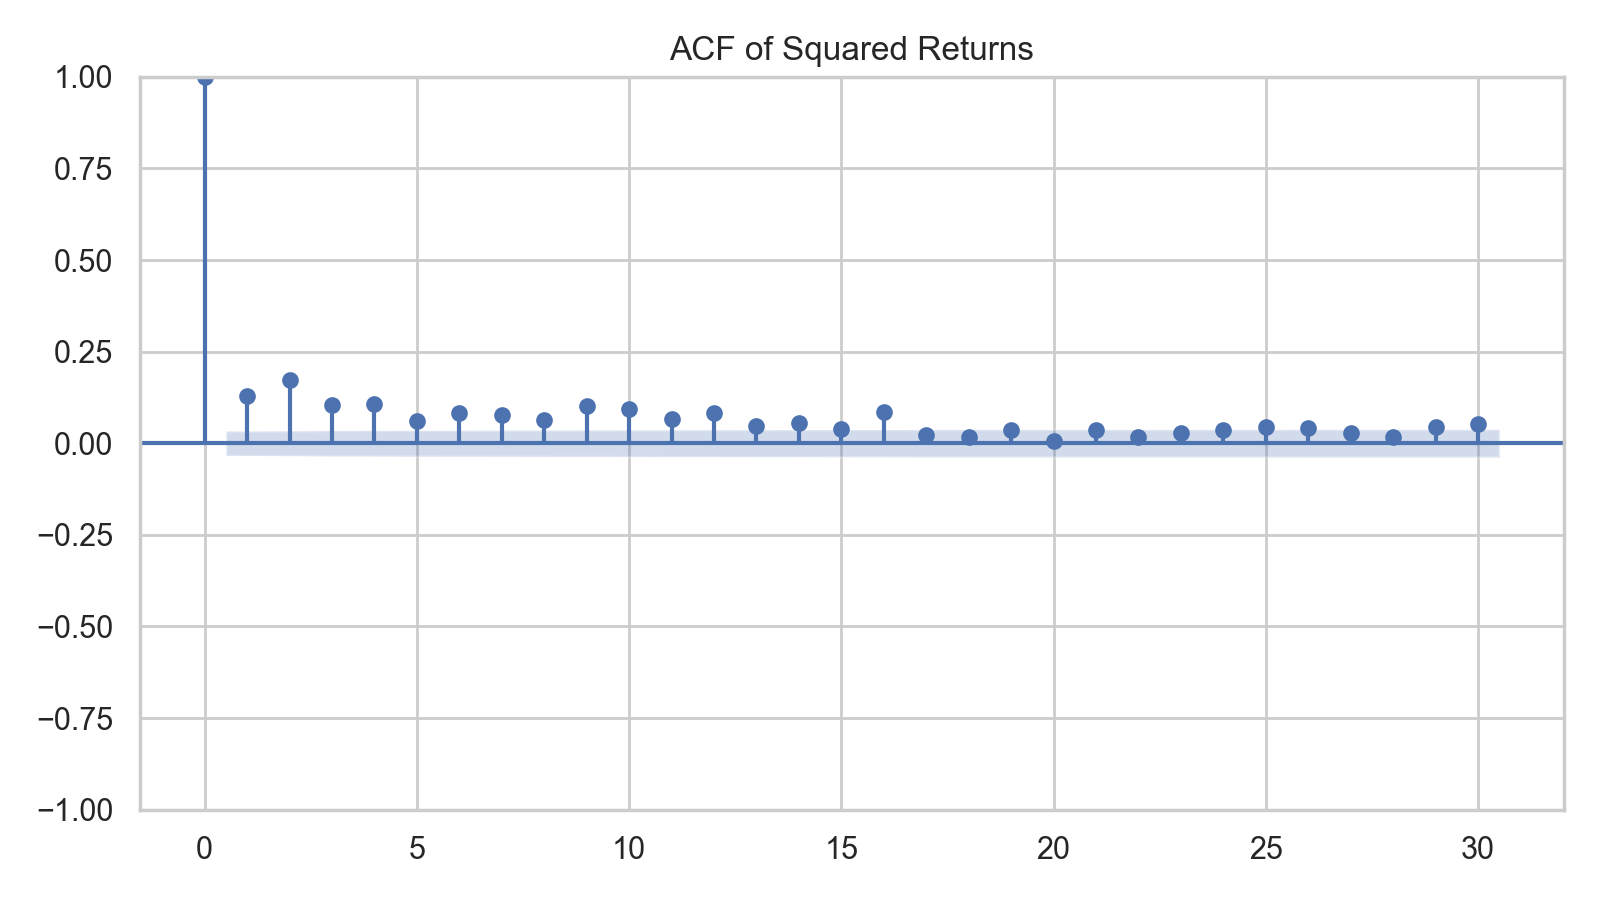
\includegraphics[width=\linewidth]{figure4_acf_squared_returns.png}
  \caption{ACF of squared returns}
\end{subfigure}
\caption{CLP serial-correlation diagnostics.}
\label{fig:clp-acf}
\end{figure}

\begin{table}[H]
\centering
\small
\csvtab{../output/clp/tables/table2_stationarity_tests.csv}
\caption{CLP stationarity tests.}
\label{tab:clp-stat}
\end{table}

\subsection{ARMA Mean Model}
We searched ARMA$(p,q)$ over $p,q\in\{0,1,2,3\}$ using BIC.  The
preferred model is \textbf{ARMA(0,0)}: the constant mean is
sufficient.  This is consistent with CLP being a defensive utility
with weak short-run mean dependence.  Residual diagnostics are
not perfect in mean, but they still support a parsimonious choice:
the residual Ljung--Box statistic is borderline at lag~10
($p=0.0486$) and insignificant at lag~20 ($p=0.0735$).  In other
words, there may be a small amount of short-run dependence, but it is
economically weak and does not justify a higher-order ARMA once BIC
penalization is taken into account.  By contrast, the remaining ARCH
effect is extremely strong: ARCH-LM~$=267.19$,
$p \approx 1.3\!\times\!10^{-51}$.  The main modelling problem for CLP
is therefore not the conditional mean, but the conditional variance.

\begin{table}[H]
\centering
\small
\adjustbox{max width=\linewidth}{%
\begin{tabular}{lrrrrr}
\toprule
Model & $p$ & $q$ & AIC & BIC & LB(10) $p$ \\
\midrule
ARMA(0,0) & 0 & 0 & 7989.13 & 8001.11 & 0.0486 \\
ARMA(0,1) & 0 & 1 & 7989.63 & 8007.60 & 0.0968 \\
ARMA(1,0) & 1 & 0 & 7989.66 & 8007.64 & 0.0957 \\
ARMA(0,2) & 0 & 2 & 7991.25 & 8015.22 & 0.0989 \\
ARMA(1,1) & 1 & 1 & 7991.26 & 8015.22 & 0.1036 \\
ARMA(2,0) & 2 & 0 & 7991.28 & 8015.25 & 0.0979 \\
ARMA(3,0) & 3 & 0 & 7992.86 & 8022.82 & 0.1177 \\
ARMA(0,3) & 0 & 3 & 7992.93 & 8022.89 & 0.1154 \\
\bottomrule
\end{tabular}%
}
\caption{CLP ARMA candidate ranking (top of the BIC table).}
\label{tab:clp-arma}
\end{table}

\subsection{Volatility Model}
GARCH(1,1), EGARCH(1,1) and GJR-GARCH(1,1) were estimated on the
mean-adjusted series.  By AIC and BIC the preferred specification is
\textbf{EGARCH(1,1)}: persistence proxy $\approx 0.953$, magnitude
term $\alpha_1 = 0.206$, asymmetry term $\gamma_1 = -0.031$.  The
small negative $\gamma_1$ suggests mild asymmetry -- bad news may
raise future volatility slightly more than good news of the same size,
even for a defensive utility.  The important result here is the high
volatility persistence: once CLP enters a turbulent period, volatility
reverts only gradually rather than immediately.

\begin{figure}[H]
\centering
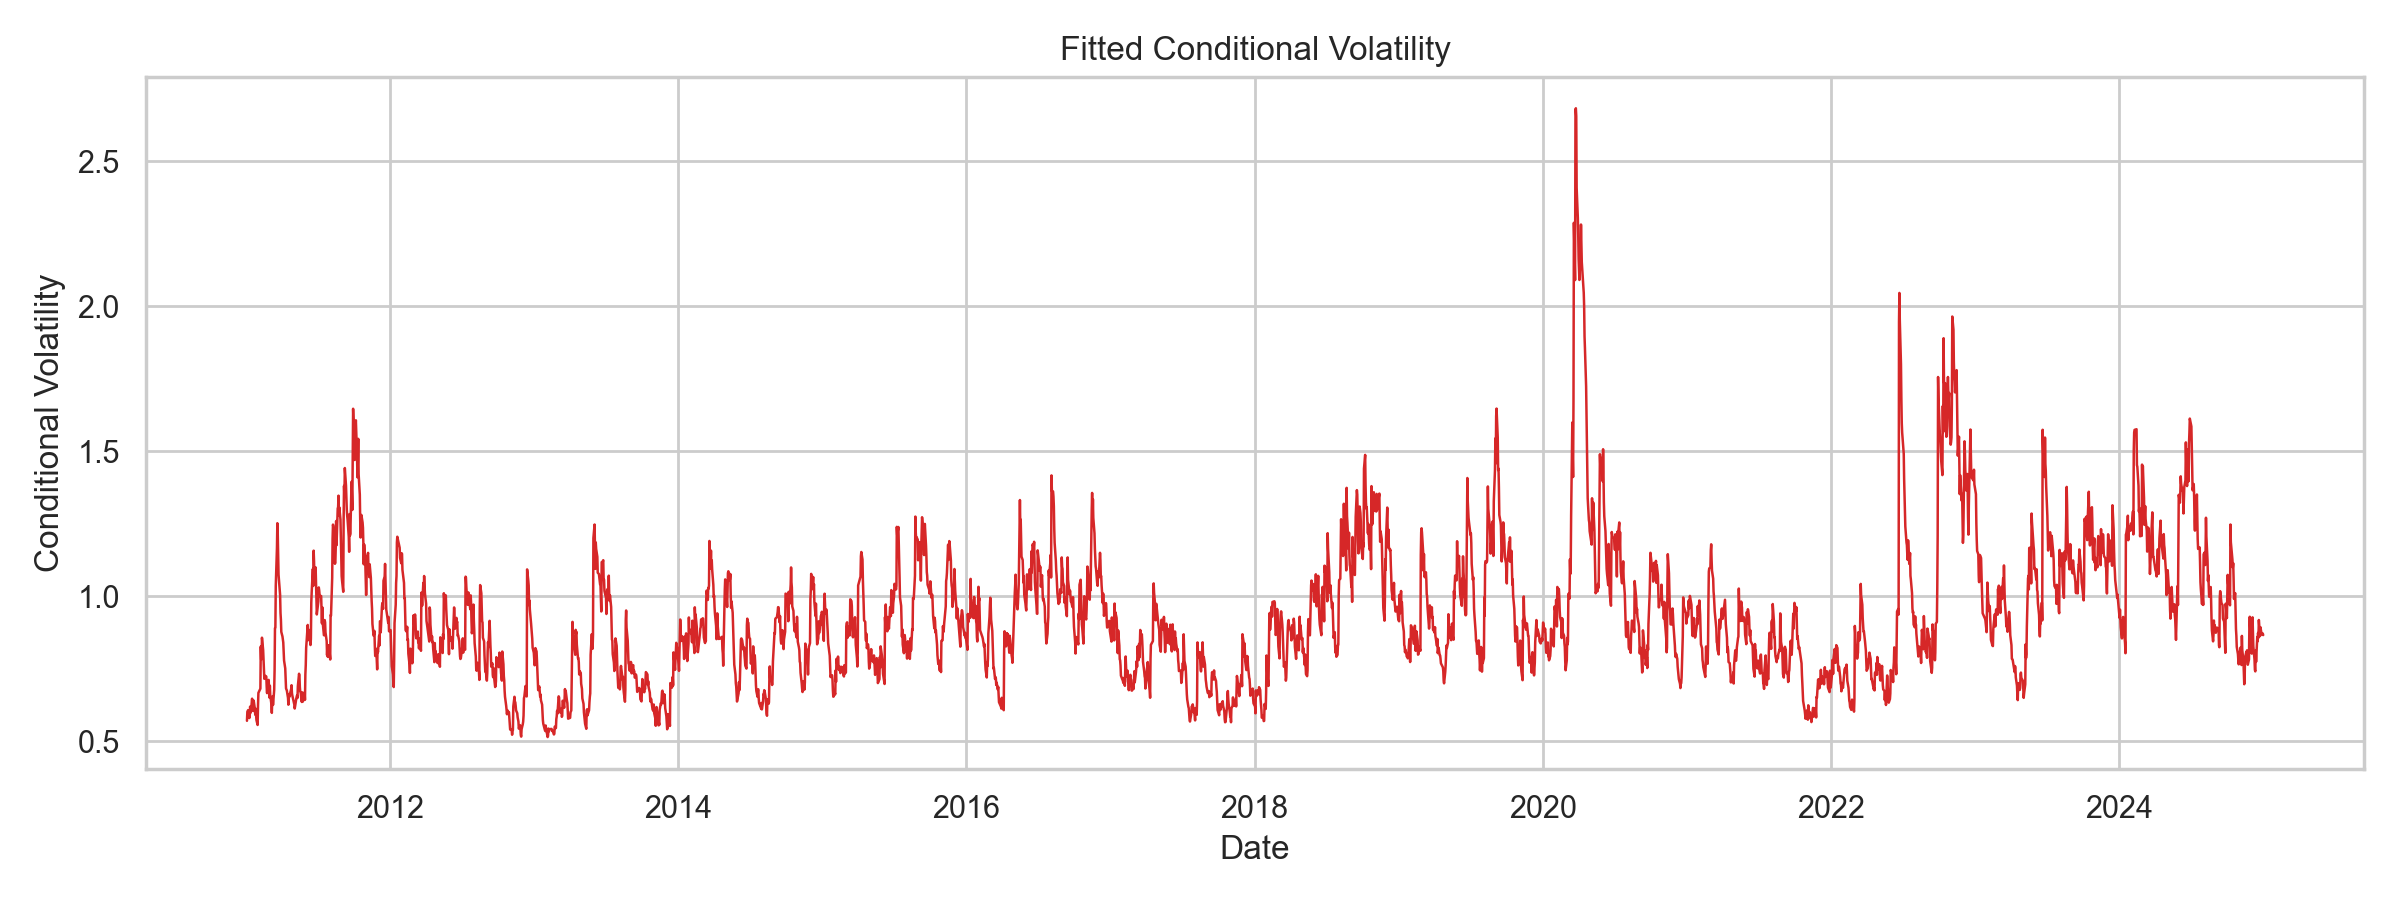
\includegraphics[width=0.95\linewidth]{figure5_conditional_volatility.png}
\caption{CLP fitted conditional volatility (EGARCH(1,1)).}
\label{fig:clp-vol}
\end{figure}

\begin{table}[H]
\centering
\small
\adjustbox{max width=\linewidth}{%
\begin{tabular}{lrrrrrrr}
\toprule
Model & AIC & BIC & $\omega$ & $\alpha_1$ & $\beta_1$ & $\gamma_1$ & Persistence \\
\midrule
EGARCH(1,1)    & 21173.67 & 21203.63 & 0.2175 & 0.2061 & 0.9525 & -0.0312 & 0.9525 \\
GARCH(1,1)     & 21195.16 & 21219.13 & 3.9395 & 0.1020 & 0.8558 & --      & 0.9578 \\
GJR-GARCH(1,1) & 21194.93 & 21224.89 & 4.0853 & 0.0847 & 0.8559 & 0.0282  & 0.9548 \\
\bottomrule
\end{tabular}%
}
\caption{CLP GARCH-family model comparison.}
\label{tab:clp-garch}
\end{table}

\subsection{Forecasting}
For out-of-sample mean forecasting on the 2023--2024 hold-out window,
we compare two rolling one-step benchmarks: ARMA(0,0) and a simple
AR-GARCH specification.  This forecast comparison is intentionally
more conservative than the in-sample volatility-selection exercise:
EGARCH(1,1) is preferred for describing CLP's conditional variance,
whereas the forecasting table asks the narrower question of whether a
standard GARCH recursion improves one-step return prediction.

The answer is: only marginally.  RMSE improves from $1.13142$ to
$1.13113$, but MAE is slightly worse for AR-GARCH, and directional
accuracy is $0.4806$ for both models.  Thus, adding a volatility model
does not make CLP's daily return direction meaningfully more
predictable.  What it adds is a better description of time-varying
risk, not a stronger forecast of the conditional mean.

\begin{figure}[H]
\centering
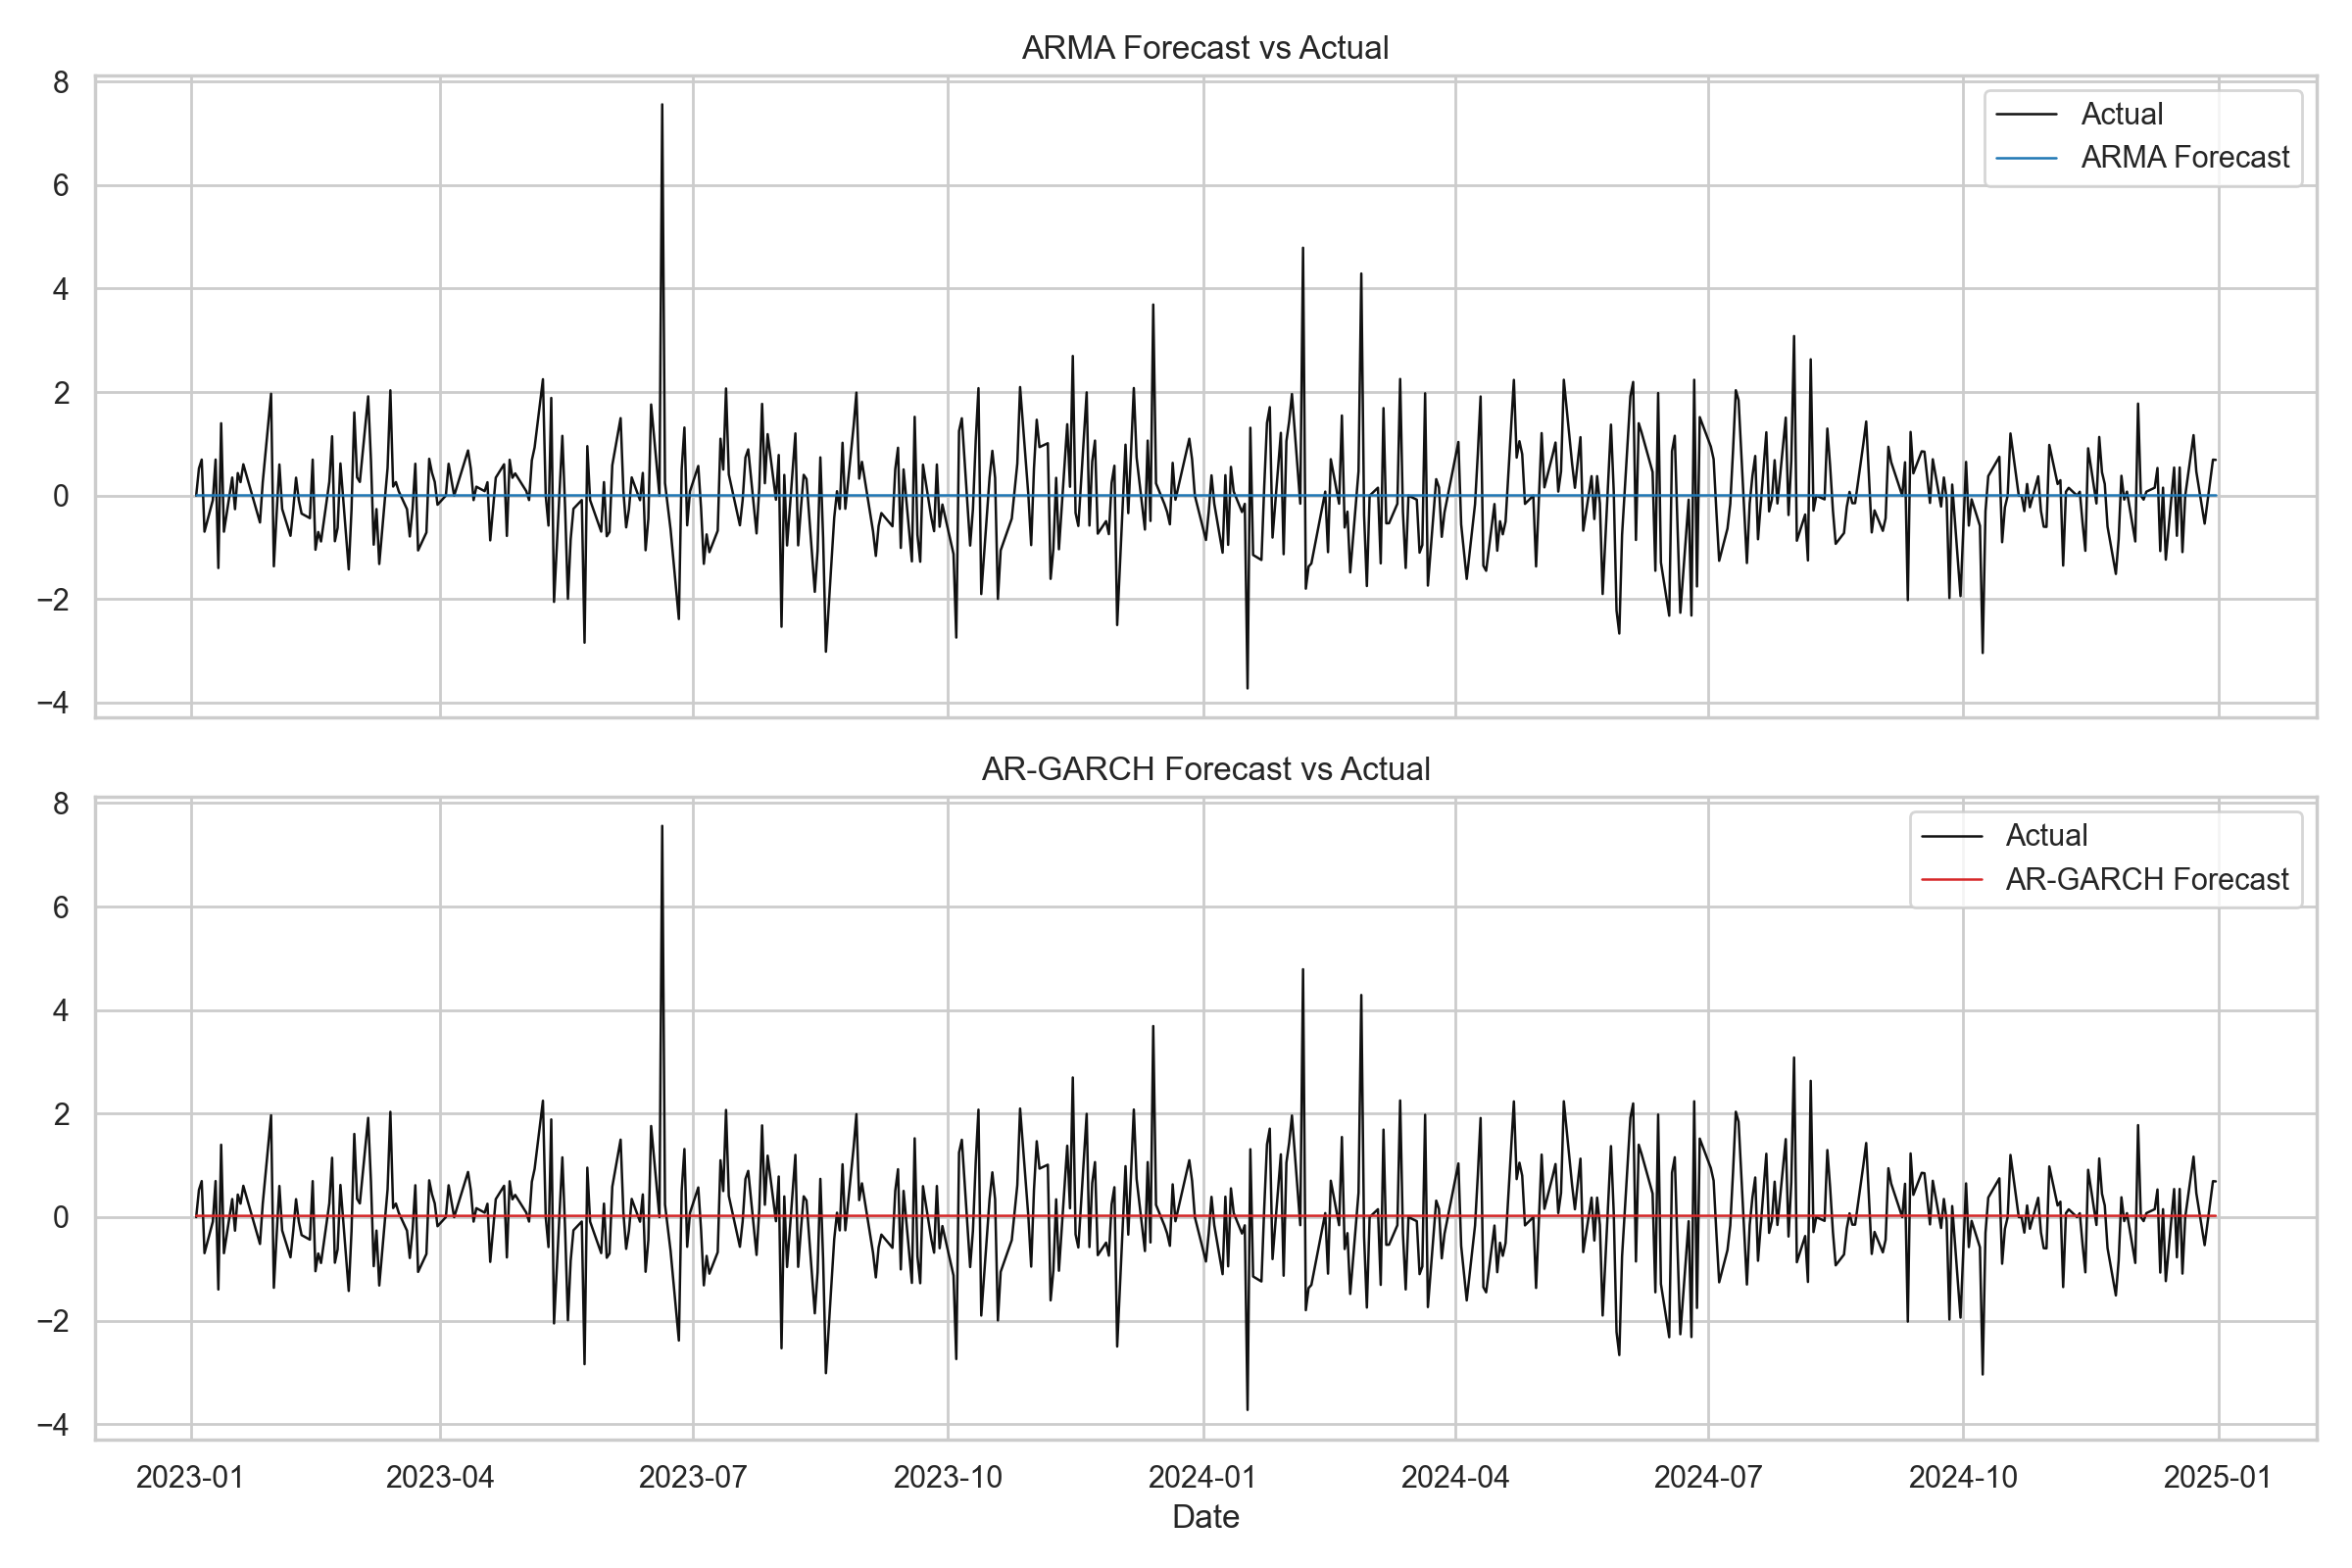
\includegraphics[width=0.95\linewidth]{figure6_forecast_vs_actual.png}
\caption{CLP one-step-ahead forecast vs actual (2023--2024).}
\label{fig:clp-fc}
\end{figure}

\begin{table}[H]
\centering
\small
\csvtab{../output/clp/tables/table5_forecasting_performance.csv}
\caption{CLP out-of-sample forecasting performance.}
\label{tab:clp-fc}
\end{table}

\subsection{Individual Conclusion -- CLP}
Prices are non-stationary, returns are stationary, mean dependence is
weak enough that a constant-mean specification is adequate for the
main analysis, while the residual ARCH effect is unambiguously strong.
Among the competing variance models, EGARCH(1,1) gives the best
in-sample fit and indicates persistent volatility with only mild
asymmetry.  Out of sample, however, even an AR-GARCH benchmark
improves return-forecast accuracy only trivially.  The economic read is
therefore clear: for CLP, predictability lives mainly in
\emph{time-varying risk} rather than in \emph{daily return direction}.
That is why CLP is the right defensive anchor for the four-stock
comparison in Section~\ref{sec:compare}.

% =====================================================================
\section{Comparative and Multivariate Results}
\label{sec:compare}

This section brings the four stocks together as a panel, in the
same order used in the project workflow: data merging, cross-stock
summary table, correlation matrix, and VAR / Granger causality.  The
joint discussion at the end synthesizes the four single-stock studies
into one group result.

\subsection{Merged Log-Return Panel}
\label{sec:compare-merge}
The four daily log-return series are aligned on common trading days
into \texttt{data/hk4\_log\_returns\_merged\_common\_dates.csv}, with
columns \texttt{date, log\_return\_hsbc, log\_return\_aia,
log\_return\_tencent, log\_return\_clp}.  The first row (2011-01-03)
contains \texttt{NaN}s by construction because of the
first-difference; we drop it before any joint analysis.  After this
cleaning step, the effective common-date sample contains
$3{,}446$ synchronized daily observations from 2011-01-04 to
2024-12-31.

This alignment step is not a mechanical appendix task but a necessary
condition for valid multivariate analysis.  Correlation matrices,
VAR models and Granger-causality tests all require that the four
series be observed on the same dates, so we use the intersection of
trading days rather than filling missing values or mixing asynchronous
observations.  The merged panel therefore ensures that any estimated
cross-stock relationship reflects genuine co-movement in returns,
not artifacts from misaligned calendars.  It also provides the single
common input used consistently by the later correlation and VAR
sections, so all multivariate results are directly comparable.

\subsection{Cross-Stock Summary Table}
\label{sec:compare-table}
We compile, in one table, each stock's preferred ARMA order,
preferred GARCH-family model, GARCH persistence, asymmetry term,
and out-of-sample RMSE / MAE / directional accuracy.  This table is
intended to summarize, in a directly comparable format, how the four
stocks differ in mean dynamics, volatility persistence, asymmetry and
forecast performance.

Table~\ref{tab:cross_stock_summary} summarizes the stock-specific results from Sections~4--7 in a single directly comparable format. The table reports each stock's preferred ARMA mean specification, preferred GARCH-family volatility model, volatility persistence, asymmetry term, and best available out-of-sample return-forecasting performance over the 2023--2024 test period. Forecast errors are measured on the daily log-return scale in percentage points.

\begin{table}[htbp]
    \centering
    \caption{Cross-stock comparison of mean dynamics, volatility structure and forecasting performance.}
    \label{tab:cross_stock_summary}
    \small
    \resizebox{\textwidth}{!}{%
    \begin{tabular}{llrrrrr}
        \hline
        Stock & Preferred models & Persistence & Asymmetry & RMSE & MAE & Directional acc. (\%) \\
        \hline
        HSBC (0005.HK) &
        ARMA(2,2); EGARCH(1,1) &
        0.9870 &
        0.0000 &
        1.2399 &
        0.8846 &
        52.05 \\
        AIA (1299.HK) &
        ARMA(1,1); GJR-GARCH(1,1) &
        0.9520 &
        0.0453 &
        1.9396 &
        1.4400 &
        46.31 \\
        Tencent (0700.HK) &
        ARMA(0,3); ARMA-GJR-GARCH(1,1) &
        0.9253 &
        0.0853 &
        2.0695 &
        1.5433 &
        50.00 \\
        CLP (0002.HK) &
        ARMA(0,0); EGARCH(1,1) &
        0.9525 &
        -0.0312 &
        1.1311 &
        0.8333 &
        48.06 \\
        \hline
    \end{tabular}%
    }
\end{table}

The comparison highlights four main cross-sectional differences. First, mean dynamics are weak across the whole sample: the selected ARMA orders are low, and CLP is adequately described by a constant-mean ARMA(0,0) specification. Second, volatility persistence is high for all four stocks, with HSBC showing the strongest volatility memory and Tencent the lowest persistence among the selected models. Third, asymmetry is most visible for Tencent and AIA, where the positive GJR leverage terms indicate that negative return shocks increase future volatility more strongly than positive shocks of similar size. HSBC has essentially no estimated asymmetry, while CLP shows only mild asymmetry under EGARCH. Finally, forecast performance is mainly ranked by each stock's underlying volatility: CLP has the lowest RMSE and MAE because it is the defensive low-volatility stock, whereas Tencent has the highest forecast errors. Directional accuracy remains close to 50\% for all four stocks, so the main value of the ARMA--GARCH framework is better risk modelling rather than reliable short-horizon direction prediction.


\subsection{Correlation Matrix}
\label{sec:compare-corr}

The $4 \times 4$ Pearson correlation matrix of daily log returns is
computed over $3{,}446$ common trading days (2011-01-04 to 2024-12-31).
All returns are in percentage form ($100 \times \Delta \ln P$).  The
matrix is presented in Table~\ref{tab:corr-matrix} and visualized as a
heatmap in Figure~\ref{fig:corr-heatmap}.

\begin{table}[H]
\centering
\small
\begin{tabular}{lcccc}
\toprule
& \textbf{HSBC} & \textbf{AIA} & \textbf{Tencent} & \textbf{CLP} \\
\midrule
HSBC (0005.HK)    & 1.0000 & 0.4833 & 0.3616 & 0.3135 \\
AIA (1299.HK)     & 0.4833 & 1.0000 & 0.4718 & 0.3661 \\
Tencent (0700.HK) & 0.3616 & 0.4718 & 1.0000 & 0.2118 \\
CLP (0002.HK)     & 0.3135 & 0.3661 & 0.2118 & 1.0000 \\
\bottomrule
\end{tabular}
\caption{Pearson correlation matrix of daily log returns.}
\label{tab:corr-matrix}
\end{table}

\begin{figure}[H]
\centering

\includegraphics[width=0.65\linewidth]{fig7_correlation_heatmap.png}
\caption{Correlation heatmap (RdBu\_r colormap).  Financial-sector
clustering is clearly visible in the top-left block; the technology--utility
pair shows the weakest co-movement.}
\label{fig:corr-heatmap}
\end{figure}

\paragraph{Key findings.}
All six pairwise correlations are positive, confirming the existence
of a common Hong Kong market factor.  The magnitude, however, varies
substantially across sector pairs:

\begin{itemize}[leftmargin=*]
  \item \textbf{HSBC--AIA ($r = 0.483$):} The strongest correlation,
        consistent with both stocks belonging to the financial sector
        and sharing exposure to interest-rate expectations and credit
        cycles.  From a portfolio perspective, the $r^2 \approx 0.23$
        implies that an equally weighted Hong Kong financials portfolio
        retains substantial sector concentration risk.
  \item \textbf{AIA--Tencent ($r = 0.472$):} Nearly as strong as the
        within-financials pair, suggesting that AIA occupies an
        intermediate position in the market -- it shares the
        financial-sector factor with HSBC while also exhibiting
        sensitivity to the broader Hang Seng growth dynamics captured
        by Tencent.
  \item \textbf{Tencent--HSBC ($r = 0.362$):} Notably lower than
        AIA--Tencent, reflecting the greater sectoral distance between
        technology and traditional banking.
  \item \textbf{Tencent--CLP ($r = 0.212$):} The weakest correlation,
        consistent with the diametrically different business models:
        Tencent is a high-growth technology stock driven by earnings
        momentum and regulatory sentiment, while CLP is a defensive
        utility with regulated, bond-like cash flows.  The low
        $r^2 \approx 0.045$ implies that a Tencent--CLP pair offers
        the strongest diversification benefit within a Hong Kong
        equity portfolio.
  \item \textbf{CLP with financials ($r = 0.31$--$0.37$):} Moderate
        correlations reflecting shared macro exposure (Hong Kong GDP,
        interest rates) but distinct sector-level return drivers.
\end{itemize}

\paragraph{Economic interpretation.}
The correlation structure supports a multi-factor interpretation of
Hong Kong equity returns: a common market factor generates uniformly
positive correlations, while sector-specific factors drive the
cross-sectional dispersion.  The financial-sector cluster (HSBC--AIA)
and the technology--utility divergence are the two most salient
features.  For risk management, the key message is that meaningful
diversification benefits exist \emph{within} a Hong Kong equity basket,
but concentrated financial-sector holdings bear significant
undiversified sector risk.

\subsection{VAR($p$) Model}

A VAR model was fitted to the four-stock log-return system including HSBC,
AIA, Tencent and CLP. Based on the selected lag order, the estimated VAR
coefficients are reported in Table~\ref{tab:var_coef}. The table shows that
most lagged return coefficients are statistically insignificant at the 5\%
level. The most important significant dynamic effects are found in the AIA
and Tencent equations.

\begin{table}[H]
\centering
\caption{Estimated VAR coefficients}
\label{tab:var_coef}
{
\begin{tabular}{llrrrr}
\toprule
Equation & Variable & Estimate & Std. Error & t value & p-value \\
\midrule
HSBC & HSBC.l1    &  0.0193 & 0.0200 &  0.9641 & 0.3351 \\
HSBC & AIA.l1     &  0.0286 & 0.0169 &  1.6894 & 0.0912 \\
HSBC & Tencent.l1 & -0.0010 & 0.0125 & -0.0762 & 0.9393 \\
HSBC & CLP.l1     & -0.0310 & 0.0268 & -1.1570 & 0.2474 \\
HSBC & const      &  0.0185 & 0.0237 &  0.7822 & 0.4342 \\

AIA & HSBC.l1     & -0.0471 & 0.0253 & -1.8564 & 0.0635 \\
AIA & AIA.l1      & -0.0344 & 0.0214 & -1.6044 & 0.1087 \\
AIA & Tencent.l1  &  0.0713 & 0.0158 &  4.5006 & $<0.001$ \\
AIA & CLP.l1      & -0.0046 & 0.0339 & -0.1353 & 0.8924 \\
AIA & const       &  0.0294 & 0.0300 &  0.9810 & 0.3266 \\

Tencent & HSBC.l1    & -0.0549 & 0.0314 & -1.7487 & 0.0804 \\
Tencent & AIA.l1     & -0.0191 & 0.0265 & -0.7187 & 0.4723 \\
Tencent & Tencent.l1 &  0.0458 & 0.0196 &  2.3367 & 0.0195 \\
Tencent & CLP.l1     & -0.0684 & 0.0420 & -1.6304 & 0.1031 \\
Tencent & const      &  0.0748 & 0.0371 &  2.0150 & 0.0440 \\

CLP & HSBC.l1     & -0.0242 & 0.0139 & -1.7433 & 0.0814 \\
CLP & AIA.l1      &  0.0122 & 0.0117 &  1.0358 & 0.3004 \\
CLP & Tencent.l1  &  0.0026 & 0.0087 &  0.3008 & 0.7636 \\
CLP & CLP.l1      & -0.0265 & 0.0186 & -1.4252 & 0.1542 \\
CLP & const       &  0.0173 & 0.0164 &  1.0548 & 0.2916 \\
\bottomrule
\end{tabular}
}
\end{table}

From Table~\ref{tab:var_coef}, Tencent's lagged return has a significant
positive effect on AIA's return, with an estimated coefficient of 0.0713 and
a p-value below 0.001. Tencent's own lagged return is also significant in the
Tencent equation, with a coefficient of 0.0458 and a p-value of 0.0195. This
suggests that Tencent contains the clearest short-run predictive information
in the fitted VAR system. Some HSBC-related lagged effects are marginally
significant at the 10\% level, but they are not significant at the 5\% level.

\begin{table}[H]
\centering
\caption{Residual diagnostic tests for the VAR model}
\label{tab:var_diag}
\begin{tabular}{lrrl}
\toprule
Test & Statistic & p-value & Conclusion at 5\% \\
\midrule
Portmanteau serial correlation test & 348.4738 & $<0.001$ & Reject $H_0$ \\
Multivariate ARCH test              & 1800.0464 & $<0.001$ & Reject $H_0$ \\
Jarque--Bera normality test          & 17406.8098 & $<0.001$ & Reject $H_0$ \\
\bottomrule
\end{tabular}
\end{table}

The residual diagnostic results in Table~\ref{tab:var_diag} show that all
three null hypotheses are rejected at the 5\% level. The Portmanteau test
indicates that residual serial correlation remains in the fitted system. The
multivariate ARCH test suggests strong conditional heteroskedasticity, which
is common in financial return data. The Jarque--Bera test rejects residual
normality, indicating that the residuals are heavy-tailed or non-Gaussian.
Therefore, although the VAR model captures part of the linear dynamic
dependence, the residual diagnostics suggest that volatility clustering and
non-normality are still present.

\begin{figure}[H]
\centering

\includegraphics[width=0.8\textwidth]{IRF_2x2_four_stock_shocks.png}
\caption{Impulse response functions for shocks from HSBC, AIA, Tencent and CLP}
\label{fig:var_irf}
\end{figure}

Figure~\ref{fig:var_irf} reports the impulse response functions of the four
stock returns. The strongest responses occur immediately at horizon 0, mainly
through each stock's own shock. After horizon 1, the responses quickly move
towards zero and become almost negligible after around two periods. This
suggests that shocks in the four-stock return system are short-lived rather
than persistent. Overall, the IRF results indicate that the VAR system is
dynamically stable, with only temporary shock transmission across the four
stocks.


\subsection{Joint Discussion}
\label{sec:compare-joint}
The four single-stock studies point to a consistent volatility ranking.
By unconditional standard deviation, \textbf{Tencent} is the most
volatile name ($\sigma \approx 2.18\%$ daily), followed by
\textbf{AIA} ($\approx 1.76\%$), \textbf{HSBC} ($\approx 1.39\%$) and
\textbf{CLP} ($\approx 0.96\%$).  This ordering is economically
plausible: technology is the most sentiment- and regulation-sensitive
sector in the sample, utilities are the most defensive, and the two
financials lie in between.  The GARCH-family results tell the same
story.  All four names show persistent conditional heteroskedasticity,
but asymmetry is strongest where the business model is most exposed to
cyclical news and market sentiment, especially Tencent and AIA, while
CLP remains the low-volatility anchor of the group.

Predictability, however, must be defined carefully.  If ``predictable''
means low forecast error in one-step-ahead returns, then CLP looks
easiest because its raw volatility is lowest, so even a simple model
produces the smallest RMSE.  If ``predictable'' means correctly calling
daily direction, then \textbf{HSBC} performs best, but only marginally,
with directional accuracy around $52\%$.  That is still too weak to
support a strong market-timing claim.  The project-wide conclusion is
therefore that none of the four stocks is meaningfully predictable in
its \emph{mean}; the real predictive content lies in the
\emph{variance}, where GARCH-type models consistently improve the
description of time-varying risk.

For cross-stock dependence, the strongest evidence is contemporaneous
rather than strongly dynamic.  All six pairwise correlations are
positive, with the tightest linkage between HSBC and AIA and the
weakest between Tencent and CLP, indicating one common Hong Kong market
factor overlaid with sector structure.  This means that intra-HK
spillover exists first as shared market movement and only second, if at
all, as a lead--lag effect.  Put differently, the data support
co-movement much more clearly than they support strong return
predictability from one stock to another.  That synthesis is the main
group result: time-series modeling in this four-stock HK sample is most
useful for measuring persistence, asymmetry and diversification
structure, rather than for extracting reliable short-horizon directional
signals.

% =====================================================================
\section{Conclusion}
\label{sec:conclusion}

\begin{itemize}[leftmargin=*]
  \item Across all four HK stocks, log prices are non-stationary while
        log returns are stationary -- the textbook result holds out of
        sample.
  \item Mean predictability is consistently weak.  ARMA orders are
        low or zero, and out-of-sample directional accuracy stays
        close to $50\%$.
  \item Conditional heteroskedasticity is strong everywhere.  EGARCH
        or GJR-GARCH is preferred for the names where bad news
        plausibly hurts more (financials, tech), while a basic
        symmetric GARCH is enough for the defensive utility.
  \item The economic message of the project is therefore: in HK
        equities, time-series modelling buys you a much better grip on
        \emph{risk} than on \emph{direction}, and the size of that
        gain scales with how cyclical / sentiment-driven the stock is.
\end{itemize}

% =====================================================================
\appendix
\section{Appendix}
\label{sec:appendix}

\subsection{Data Files}
All data lives under \texttt{data/} and is fully reproducible from
Yahoo Finance.

\begin{table}[H]
\centering
\small
\begin{tabular}{lll}
\toprule
File & Content & Used in \\
\midrule
\texttt{<ticker>\_yahoo\_raw.csv}            & raw OHLCV download           & data lineage \\
\texttt{<ticker>\_adjusted\_close\_2011\_2024.csv} & cleaned adjusted close   & per-stock analysis \\
\texttt{hk4\_log\_returns\_merged\_common\_dates.csv} & merged 4-stock returns & \S\ref{sec:compare} \\
\bottomrule
\end{tabular}
\caption{Data files in \texttt{data/}.  \texttt{<ticker>} is one of
\texttt{0005\_HK\_hsbc}, \texttt{1299\_HK\_aia},
\texttt{0700\_HK\_tencent}, \texttt{0002\_HK\_clp}.}
\end{table}

\subsection{Per-Stock Result Tables (CSV)}
All numeric results referenced in
Sections~\ref{sec:hsbc}--\ref{sec:clp} are persisted as CSV under
\texttt{output/<ticker>/tables/} and reproduced verbatim in the main
text via \texttt{csvsimple}.  Filenames are stable across the four
stocks:
\begin{itemize}[leftmargin=*]
  \item \texttt{table1\_descriptive\_statistics.csv}
  \item \texttt{table2\_stationarity\_tests.csv}
  \item \texttt{table2b\_residual\_diagnostics.csv}
  \item \texttt{table3\_arma\_candidates.csv}
  \item \texttt{table4\_garch\_models.csv}
  \item \texttt{table5\_forecasting\_performance.csv}
  \item \texttt{forecast\_series.csv}
\end{itemize}

\subsection{Per-Stock Figures (PNG)}
Identically named PNG figures live under
\texttt{output/<ticker>/figures/}: \texttt{figure1\_price\_and\_log\_price.png},
\texttt{figure2\_log\_return\_plot.png},
\texttt{figure3\_acf\_pacf\_returns.png},
\texttt{figure4\_acf\_squared\_returns.png},
\texttt{figure5\_conditional\_volatility.png},
\texttt{figure6\_forecast\_vs\_actual.png}.

\subsection{Author Contributions}
The report was prepared collaboratively, with the following primary
responsibilities:
\begin{itemize}[leftmargin=*]
  \item \textbf{Author 1} -- HSBC (\S\ref{sec:hsbc}) and the
        cross-stock summary table (\S\ref{sec:compare-table}).
  \item \textbf{Author 2} -- AIA (\S\ref{sec:aia}) and the
        correlation matrix (\S\ref{sec:compare-corr}).
  \item \textbf{Author 3} -- Tencent (\S\ref{sec:tencent}) and
        the VAR / Granger-causality analysis
        (\S\ref{sec:compare-var}).
  \item \textbf{Author 4} -- CLP (\S\ref{sec:clp}), the merged
        log-return panel (\S\ref{sec:compare-merge}) and joint
        discussion coordination.
\end{itemize}

\end{document}
